\documentclass[PhD,Submit,ngerman,UKenglish]{scrbook}
%------------------------------------------------------------------------------
% This file contains a skeleton thesis for
% a Physics or Astronomy Institute in the University of Bonn

% Specify the thesis type as an option: PhD, Master, Diplom, Bachelor
% Specify the thesis stage as an option: Draft (default), Submit, Final, PILibrary

% Specify the language(s) in the class and then use babel.
% If you need more than one language, give the default language last,
% e.g. ngerman,UKenglish for a thesis in British (UK) English where you want
% to be able to set the language to German for some part of it.

%------------------------------------------------------------------------------
% Pass TeX Live version to the package
% Use command pdflatex --version to find out which version you are running
% Add option backref=false when your thesis is ready to turn off back-referencing
% in your bibliography
\usepackage[texlive=2016,biblatex=false,newtx=false,txfonts=true]{ubonn-thesis}
% Adjustments to standard biblatex style
% \usepackage{ubonn-biblatex}

% Glossary package
% \usepackage[acronym,toc,nosuper]{glossaries}
% TikZ packages and libraries
% \usepackage{tikz}
% \usepackage{tikz-3dplot}
% \usepackage{pgfplots}
% \usetikzlibrary{positioning,shapes,arrows}
% \usetikzlibrary{decorations.pathmorphing}
% \usetikzlibrary{decorations.markings}
\usepackage{thesis_defs}
\usepackage{todonotes}
\usepackage{amsmath}
\usepackage{placeins}
%------------------------------------------------------------------------------
% Instead of colouring  links, cites, table of contents etc.
% put them in a coloured box for the screen version.
% This is probably a good idea when you print your thesis.
\hypersetup{colorlinks=false,
  linkbordercolor=blue,citebordercolor=magenta,urlbordercolor=darkgreen
}

%------------------------------------------------------------------------------
% When writing your thesis it is often helpful to have the date and
% time in the output file. Comment this out for the final version.
% \ifoot[\today{} \thistime]{\today{} \thistime}

% In order to check if your labels are referenced try the refcheck package
% \usepackage{refcheck}

%------------------------------------------------------------------------------
% biblatex is included by ubonn-thesis. Look there for the settings used.
% See the options for settings that can be changed easily.
% For further changes copy the \RequirePackage[...]{biblatex} here
% and include ubonn-thesis with the option biblatex=false.

% Specify the bibliography files here and not at the end!
% Use standard_refs-bibtex if you use bibtex8
% and standard_refs-biber  if you use biber
% \addbibresource{thesis_refs.bib}
% \addbibresource{../refs/standard_refs-biber.bib}

%------------------------------------------------------------------------------
% The following definitions are used to produce the title pages
% needed at various stages
\newcommand{\thesistitle}{Event reconstruction for Dark Photon searches at NA64}
\newcommand*{\thesisauthor}{Srijan Sehgal}
\newcommand*{\thesistown}{Bonn}
\renewcommand*{\InstituteName}{\HISKP}
\renewcommand*{\inInstitute}{\inHISKP}
\renewcommand*{\InstituteAddress}{\HISKPaddress}
% Adjust \thesisreferee...text depending on male/female referee
\newcommand*{\thesisrefereeonetext}{1.\ Gutachter}
\newcommand*{\thesisrefereeone}{Prof.\ Dr.\ Bernhard Ketzer}
\newcommand*{\thesisrefereetwotext}{2.\ Gutachter}
\newcommand*{\thesisrefereetwo}{Prof.\ Dr.\ Jochen Dingfelder}
% Date when thesis was submitted (Master/Diplom)
% Year or Month, Year when thesis was submitted (PhD)
\newcommand*{\thesissubmit}{16.12.2019}
% \newcommand*{\thesissubmit}{Month 2016}
% Date of thesis examination (PhD)
\newcommand*{\thesispromotion}{16.12.2016}
% Month and year of the final printed version of the thesis
\newcommand*{\thesismonth}{December}
\newcommand*{\thesisyear}{2019}
\newcommand*{\thesisnumber}{BONN-IR-2019-XXX}

%------------------------------------------------------------------------------
% The abstract is only needed for the printed version and should be in
% English regardless of the language of the thesis
\newcommand{\thesisabstract}{%
  \begin{otherlanguage}{UKenglish}
    This is your thesis abstract. It may be in a language that is
    different from the rest of your thesis.
  \end{otherlanguage}
}

%------------------------------------------------------------------------------
% \includeonly can be used to select which chapters you want to process
% A simple \include command just inserts a \clearpage before and after the file
% Note that \includeonly can be quite picky! Do not forget to put a
% comma after the filename, otherwise it will simply be ignored!
% \includeonly{%
%   thesis_intro,
%   thesis_appendix,
%   thesis_acknowledge
% }

%------------------------------------------------------------------------------
% Give a list of directories where figures can be found. Do not leave
% any spaces in the list and end the directory name with a /
\graphicspath{%
  {../figs/}%
  {../figs/cover/}%
  {../figs/graphics/}%
  {../feynmf/}%
}

%------------------------------------------------------------------------------
% Make a glossary and a list of acronyms
% \makeglossaries

% Glossary entries
% %
% Contains a list of glossary definitions to illustrate how a glossary
% using the glossaries package
%

\newglossaryentry{siunitx}{name=siunitx,
  description={the best package around for typesetting units}}
\newglossaryentry{csquotes}{name=csquotes,
  description={a very nice package for using consistent quotes that is
  language sensitive}}
\newglossaryentry{LaTeX}{name=\LaTeX,
  description={the typesetting program that is used for this guide}}


\newacronym[plural=CRs,firstplural=cosmic rays (CRs)]{CR}{CR}{cosmic ray}  
\newacronym[plural=UHECRs,firstplural=ultra-high energy cosmic rays (UHECRs)]{UHECR}{UHECR}{ultra-high energy cosmic ray}  
\newacronym{UHE}{UHE}{ultra high energy}
\newacronym{UHEnu}{UHE$\nu$}{Ultra high energy neutrino}
\newacronym{UHEnus}{UHE$\nu$}{ultra high energy neutrinos}
\newacronym{SD}{SD}{Surface Detector}
\newacronym{FD}{FD}{Fluorescence Detector}
\newacronym{HEAT}{HEAT}{High Elevation Auger Telescope}
\newacronym[first= \textit{lateral distribution function} (LDF)]{LDF}{LDF}{lateral distribution function}
\newacronym{EM}{EM}{electromagnetic}
\newacronym{MVA}{MVA}{multivariate analysis}
\newacronym{AUGER}{AUGER}{Pierre Auger Observatory}
\newacronym[plural=EASs,firstplural= Extensive Air Showers (EASs)]{EAS}{EAS}{extensive air shower}
\newacronym{VEM}{VEM}{vertical equivalent muon}
\newacronym{MoPS}{MoPS}{Multiplicity-of-Positive-Steps}
\newacronym{FADC}{FADC}{flash analog-to-digital converter}
\newacronym{GZK}{GZK}{Greisen–Zatsepin–Kuzmi}
\newacronym{ToT}{ToT}{time-over-threshold}
\newacronym{ToTd}{ToTd}{Time-over-Threshold-deconvolved}
\newacronym{DGL}{DG$\mathrm{_{low}}$}{down-going low}
\newacronym{DGH}{DG$\mathrm{_{high}}$}{down-going high}
\newacronym{ES}{ES}{Earth-skimming}
\newacronym{TA}{TA}{Telescope Array}
\newacronym{CNB}{CNB}{Cosmic Neutrino Background}
\newacronym{CMB}{CMB}{Cosmic Microwave Background}
\newacronym{ISM}{ISM}{interstellar medium}
\newacronym{AGN}{AGN}{Active Galactic Nuclei}
\newacronym{eV}{eV}{electronvolts}
\newacronym{HESS}{HESS}{High Energy Stereoscopic System}
\newacronym{CTA}{CTA}{Cherenkov Telescope Array}
\newacronym{EBL}{EBL}{extragalactic background light}
\newacronym{WIMP}{WIMP}{Weakly Interacting Massive Particle} 
\newacronym{CC}{CC}{Charged Current}
\newacronym{NC}{NC}{Neutral Current}
\newacronym{QCD}{QCD}{quantum chromodynamics}
\newacronym{MHz}{MHz}{megahertz}
\newacronym{GHz}{GHz}{gigahertz}
\newacronym{UV}{UV}{ultraviolet}
\newacronym{IACT}{IACT}{Imaging Cherenkov telescope}
\newacronym{PMT}{PMT}{photomultiplier tube}
\newacronym{RD}{RD}{Radio Detector}
\newacronym{UMD}{UMD}{Underground Muon Detector}
\newacronym{CLF}{CLF}{Central Laser Facility}
\newacronym{XLF}{XLF}{eXtreme Laser Facility}
\newacronym{WCD}{WCD}{Water Cherenkov Detector}
\newacronym{VCT}{VCT}{vertically central through-going}
\newacronym{TH}{TH}{threshold trigger}
\newacronym{UUB}{UUB}{upgraded unified board}
\newacronym{ADST}{ADST}{Advanced Data Summary Tree}
\newacronym{AoP}{AoP}{Area over Peak}
\newacronym{MC}{MC}{Monte Carlo}
\newacronym{GDAS}{GDAS}{Global Data Assimilation System}
\newacronym{FDA}{FDA}{Fisher Discriminant Analysis}
\newacronym{LDA}{LDA}{Linear Discriminant Analysis}
\newacronym{FOV}{FOV}{field of view}





% Draft version - add DRAFT to header.
% You can use draftwatermark to add DRAFT to the cover page.
% Note that this only works if \unitlength is set to 1pt.
% This is normally not the case - it is set to 1mm in ubonn-thesis.sty.
% The background package is used for later versions of TeX Live.
%\setlength{\unitlength}{1pt}
% \ifthenelse{\equal{\ThesisVersion}{Draft}}{%
%   \usepackage{background}
%   \ifthenelse{\texlive < 2013}{%
%     \SetBgContents{DRAFT}
%     \SetBgColor{blue!30}
%   }{%
%     \backgroundsetup{contents=DRAFT, color=blue!30}
%   }
% }

%------------------------------------------------------------------------------
\begin{document}

% Cover page of thesis - this is only needed for the printed final
% version to be submitted to the department library
% Do not use this page for thesis submission to the Prüfungsamt or Promotionsbüro!
\ifthenelse{\equal{\ThesisVersion}{PILibrary}}{%
  \typeout{Document \jobname, Info: PI library version of thesis}
  \input{../cover/\ThesisType_Cover}
}{}

% Start counting pages from the title page
\frontmatter
% Dedication has to come before \maketitle
% \dedication{For ...}

% Select the correct title page(s)
\ifthenelse{\equal{\ThesisType}{Unknown}}{%
  \typeout{Document \jobname, Error: Unknown thesis type - no title page printed}
}{%
  % Bachelor thesis only has one title page
  \ifthenelse{\equal{\ThesisType}{Bachelor}}{%
    \typeout{Document \jobname, Info: Bachelor thesis}
    \input{../cover/\ThesisType_Title}
  }{%
    \ifthenelse{\equal{\ThesisVersion}{Final} \OR \equal{\ThesisVersion}{PILibrary}}{%
      % Final and PI library versions
      \typeout{Document \jobname, Info: Final version of a \ThesisType  thesis}
      \input{../cover/\ThesisType_Final_Title}
    }{% Submission and draft versions
      \input{../cover/\ThesisType_Submit_Title}
      \typeout{Document \jobname, Info: Draft/submission version of a \ThesisType  thesis}
    }
  }
}

\pagestyle{scrplain}

%------------------------------------------------------------------------------
% You can add your acknowledgements here - don't forget to also add
% them to \includeonly above
%------------------------------------------------------------------------------
\chapter*{Acknowledgements}
\label{sec:ack}
%------------------------------------------------------------------------------
Even though this thesis has my name on the front a number of people were involved in shaping its final form both in person and in spirit.

First and foremost I would like to thank my late grandfather Shanti Sarup Sehgal and grandmother Kusum Sehgal. Their constant motivation and belief in my abilities has and will always inspire me to achieve more.

I am very grateful to Professor Bernhard Ketzer for giving me an opportunity to write my thesis in his group. In spite of my many shortcomings and failures he has always been patient and supportive during the entire time and has been a role model I look up to. I would also like to thank Professor Jochen Dingfelder. I have always admired your lectures and am thankful that you agreed to be my second supervisor.

A special thanks to PhD students Michael Hösgen and Martin Hoffmann for helping with the editing of this thesis. Thank you to Michael for always answering my various questions and solving my problems without which this thesis would have never been completed. A big thanks to the whole AG Ketzer group for both the academic and moral support.

I am grateful to my father Ravi Sehgal, my mother Rajni Sehgal and my brother Sambhav for all the sacrifices they have made. Without their constant support studying at Bonn would have just remained a pipe dream. Lastly, I am thankful to the wonderful set of friends I am lucky to have. Thank you Svenja ,Georgios and Amitayus for the countless Mensa lunches which helped me remain sane throughout the thesis.

%%% Local Variables:
%%% mode: latex
%%% TeX-master: "../mythesis"
%%% End:


\tableofcontents

\mainmatter
\pagestyle{scrheadings}

% Turn off DRAFT for the following pages
%\ifthenelse{\equal{\ThesisVersion}{Draft}}{%
%  \ifthenelse{\texlive < 2013}{%
%    \SetBgContents{}
%  }{%
%    \backgroundsetup{contents={}}
%  }
%}{}

%------------------------------------------------------------------------------
% Add your chapters here - don't forget to also add them to \includeonly above
% !TEX root = mythesis.tex

%==============================================================================
\chapter{Introduction}
\label{sec:intro}
%==============================================================================
\begin{figure}[h!]
\centering
  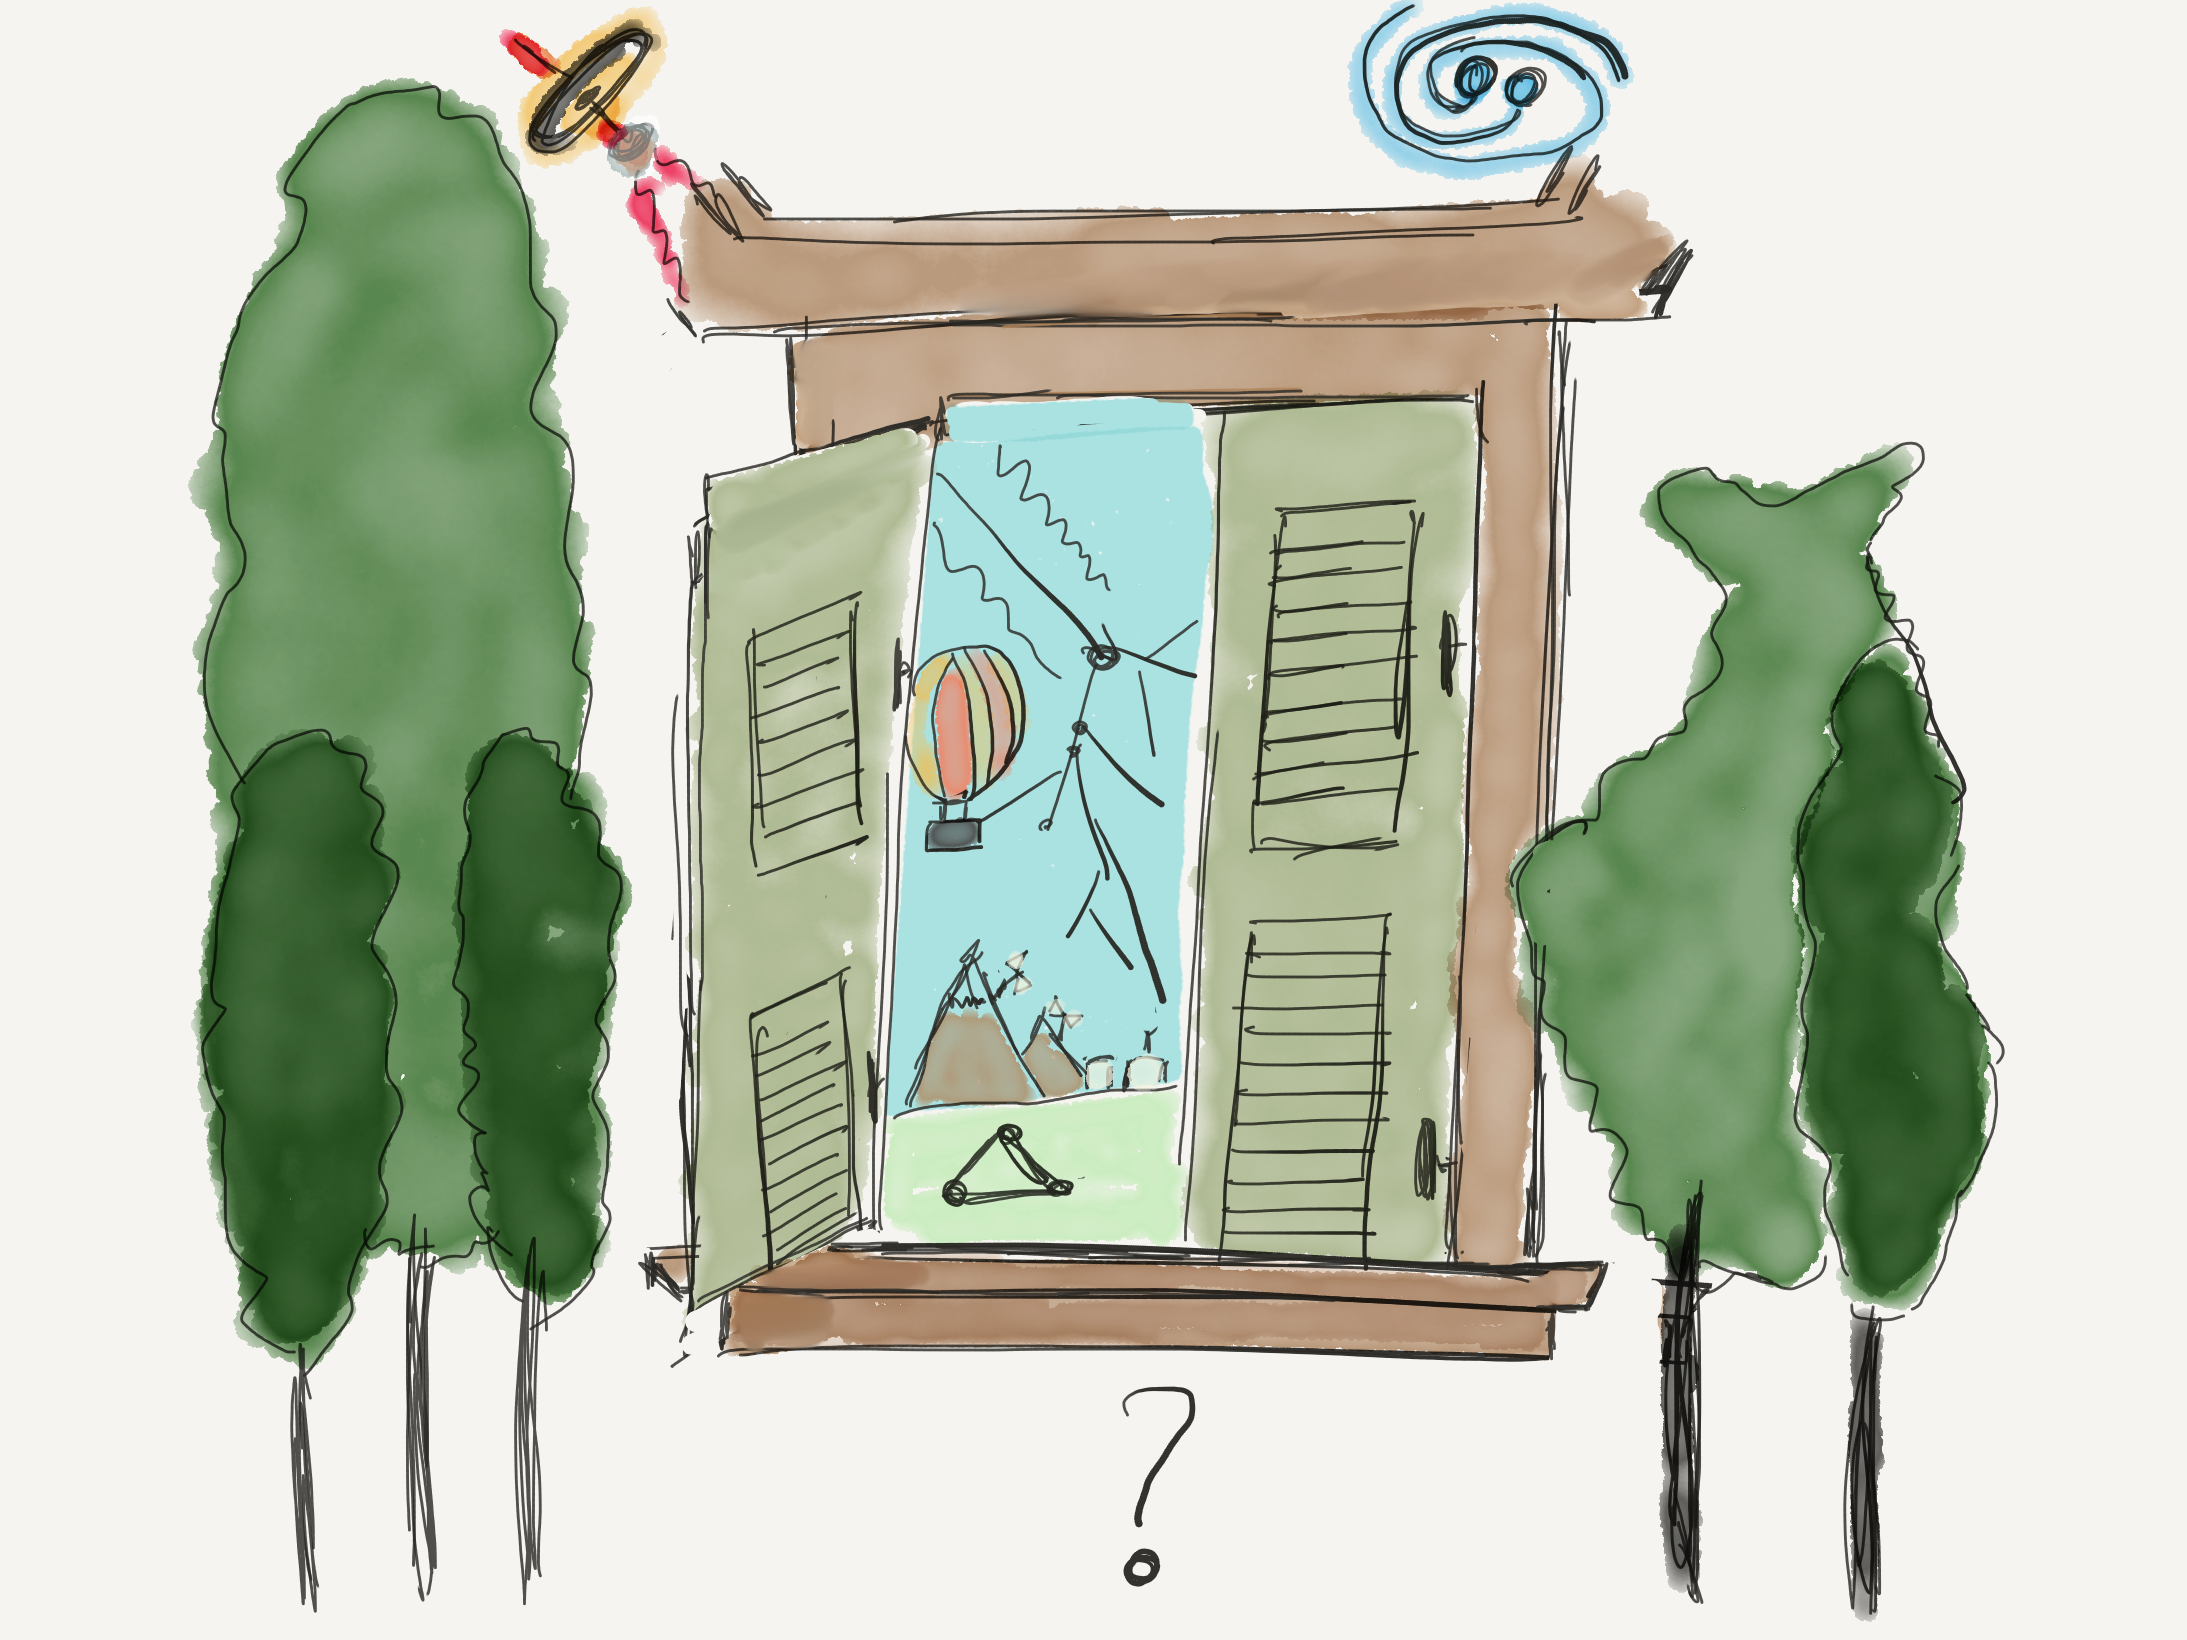
\includegraphics[width=13cm]{thesis_figures/What?.png}
\caption{Window to the inner workings of the Universe is only half opened. (better caption?)}
\label{fig:intro}
\end{figure}
The need to understand how something works or why something is? is ingrained in every human. While attempting to find answers for these questions one either answers them conclusively or finds oneself asking additional questions stemming from the original. One such question which bothered physicists at the beginning of the 20th century and eventually led to the field of \textit{astro-particle physics} was of so-called "atmosphere electricity" or ionization of air. After the pioneering discoveries by Theodor Wulf~\cite{article_Wulf} and Victor Hess~\cite{Hess:1912srp} who found the increase of this ionization rate with altitude and theorized the origin of this radiation to be not earth but something above our atmosphere, the name \textit{cosmic rays} was coined by Robert Millikan who believed these rays were originating from primary photons. This hypothesis was rejected by the measurements done by Jacob Clay~\cite{Clay:1927I,Clay:1928II} in 1927 who observed a latitude dependence of the intensity of cosmic rays concluding this to be a deflection of the primary cosmic-rays(CRs) by the geomagnetic field of the earth which indicated that these rays must be charged particles. After this came the efforts of B. Rossi~\cite{rossi1933eigenschaften}, German group~\cite{schmeiser1938harten} and P. Auger~\cite{RevModPhys.11.288} all independently discovering coincident signals in separated Geiger counters which they explained by the counters being struck by an extensive particle shower triggered by a primary cosmic ray. The phenomenon was named \textit{sciami} by Rossi, \textit{Luftshauer} by the German group and "Auger showers" by Auger and his collaborators. Auger went one step further by further estimating the primary energy of the cosmic ray via his superior setup giving rise to some questions about CRs which are yet unanswered, how are they created and where are they coming from. One of the known sources which is the Sun is too close to explain some other high energy CRs constantly hitting the Earth's atmosphere. Since then the field has only expanded with numerous experiments set up to characterize these cosmic rays. 

The biggest of these experiments which looks for ultra-high energy cosmic rays(UHECRs) exists in 3000 km$^2$ patch of Argentinian pampa just outside Malargue called the Pierre Auger Observatory~\cite{Auger:2015}. It uses a combination of 1660 Water Cherenkov tanks which form the Surface Detector of the observatory and observe the air shower particles arriving at the ground along with Fluorescence Detectors/Telescopes which can look at the development of shower as it travels through the atmosphere. Built primarily to answer the question of the cut-off of the cosmic ray spectrum also known as Greisen–Zatsepin–Kuzmin limit(or GZK cut-off), the observatory has provided immense contributions not only in the field of CRs but also in the fields of Geophysics(elves)~\cite{Mussa_2022}, Dark matter(composition)~\cite{Abreu_2023} and multi-messenger physics(neutrino+photon searches)~\cite{Aab_2019_point,Auger_photons_2022}. Currently, the Surface detector is undergoing an upgrade which will add a scintillator and radio detector on top of the Water Cherenkov tanks further increasing the sensitivity of the Observatory especially to the composition of the cosmic rays.

The non-electrical neutrality of the incoming CRs provides one of the biggest hindrance for finding their sources. This means that CRs do not travel in straight lines from their sources and are affected by the magnetic fields and can also interact with the matter along the way~\cite{bister2024largescaleanisotropyfluxdemagnification, ALLARD201233}. Combined with the fact that the possible sources are light years away from us, without knowing the magnetic fields of the Universe it is very hard to detect the sources of CRs. Ultra High Energy Neutrinos (UHE$\nu_s$) can help in this challenging search for the sources of CRs~\cite{UHEcorrelation_2016}. Being electrically neutral and having a very low interaction cross-section these particles can travel large distances unaffected by the intervening matter and magnetic fields. Several scenarios which are discussed later in section.~\ref{subsubsec:CRmessengers} describe how the UHE$\nu_s$ can be produced by cosmic-rays and can tell us about their sources. Moreover, UHE$\nu_s$ are also interesting as they can also help constrain or explain different production and propagation scenarios for various sources helping us see known astrophysical and cosmogenic objects in a new way. The success of IceCube Neutrino Observatory, a neutrino observatory located in the South Pole,  in detecting the first astrophysical neutrinos and observations of the first steady source NGC 1068~\cite{Icecube_2022} and transient source~\cite{Icecube_txs} have reinvigorated the astro-particle field. The Pierre Auger Observatory has also contributed to the search for UHE$\nu_s$ by trying to detect the Extensive Air SHowers (EASs) that can be induced by them. With its stellar sensitivity at high energy, searches at Pierre Auger Observatory have provided some of the strictest upper limits on the diffuse flux of UHE neutrinos~\cite{Aab_2019_diffuse}. This has already led to constrains on various hypothesized models explaining cosmogenic neutrino production.

The last decade with the successes of LIGO/VIRGO~\cite{PhysRevLett.116.061102} in measuring the first Gravitational waves and IceCube in detecting the first astrophysical neutrinos has also rekindled a field which displays the true spirit of harmony in science and is called multi-messenger astronomy. The aim of the field is to establish a network that can coalesce all the information available through various messengers via which we can see the Universe and maximise the resources and experiments available at Earth. This also allows us to understand the sources better since the observation or non-observation of different messengers can help constrain the mechanisms behind their functioning. The beginning of this field can be traced back to the observation of the first cosmic rays in conjunction with solar flares further cementing the important role Pierre Auger Observatory can play for this field. One of the most important success stories of this field is the August 2017 detection of the neutron star collision~\cite{Abbott_2017} first by the LIGO/VIRGO detector since the Gravitational waves are the fastest messengers and then 1.7s later by the Fermi Gamma ray space telescope and INTEGRAL. 11 hours later already alerted by these two experiments the optical counterpart was detected by multiple telescopes like Las Campanas Observatory and the Hubble Space Telescope. The event was also further seen in Ultraviolet(Neil Gehrels Swift Observatory), X-ray(Chandra X-ray Observatory) and radio(Karl G. Jansky Very Large Array). The non observation of neutrinos by both the IceCube and the Pierre Auger Observatory helped reach the important conclusion about the orientation of the jets which is hypothesized to be off-axis i.e. not pointing directly towards the Earth. Since neutrinos and Gravitational waves are the fastest of the messengers to reach the Earth, alerts issued by IceCube and LIGO/VIRGO are regularly used to follow up the events with other experiments. Subsequent observations of the blazar TXS 0506+056~\cite{TXS_Multi_2018} with IceCube, FERMI-LAT and MAGIC and the observations of neutrinos from the plane of the Milky Way galaxy~\cite{Galactic_plane_nu_2023} have helped establish the continued importance of multi-messenger astronomy.

In this thesis performance of one of the upgrades of the Pierre Auger Observatory done in 2013 is evaluated in the context of neutrino search. This upgrade consisted of introducing new triggers called Time over Threshold deconvulated(ToTd) and Multiple of Positive Steps(MoPS) to reduce the muonic background and effectively decrease the energy threshold for the array. Such triggers can be particularly important in the context of neutrino searches between $60^\circ$-$75^\circ$ since they help in getting a better signal background separation. The effect of these triggers for both the search of a diffused neutrino flux and point like sources of neutrinos is investigated. The thesis also focuses on maximising the previously done neutrino searches in the zenith region $60^\circ$-$75^\circ$ by investigating and updating the analysis presented in~\cite{Aab_2019_diffuse},~\cite{gap_note_2013}.

The thesis is structured as follows, The next chapter~\ref{chap:crnNu} gives the theoretical background for UHE cosmic rays and UHE neutrinos and other important messengers in regard to the Pierre Auger Observatory. It also aims to discuss the various theoretical scenarios involved in their production and propagation. The chapter also aims to summarize the important recent results for these messengers and the various interesting open questions for them. The next chapter~\ref{chap:EAS} describes the phenomenon of Extensive Air showers which is used to indirectly detect both the cosmic rays and neutrinos at the Pierre Auger Observatory. To continue with understanding the detection in a more experimental context the next chapter~\ref{chap:setup} gives a detailed description of the Pierre Auger Observatory. The objective of the chapter is to try to give an exhaustive description of all the tools at the Pierre Auger Observatory necessary to detect neutrinos with a particular focus on the Surface Detector which is of primary concern for the analysis presented in this thesis. A small section is also dedicated to the recently completed AugerPrime upgrade and the exciting potential it offers especially for multi-messenger searches. 

The second part of the thesis is dedicated to the neutrino search in the zenith angular region $60^\circ$-$75^\circ$ (Down-going low, DG$\mathrm{_{low}}$). This part begins with the chapter~\ref{chap:DGL} that gives a description of the neutrino search in the angular range $60^\circ$-$75^\circ$ which is also the primary focus region for this thesis. The chapter is dedicated to provide a complete description of the choices made for the analysis with the proper reasoning. It reports the areas of potential improvements and also communicates the observed improvements to the neutrino search with the new triggers. A new ~\textit{blind} search is performed to look for neutrinos in the data recorded at the Pierre Auger Observatory. The results are summarised at the end of this chapter and due to the non-observance of any neutrino like events, the corresponding limits to the neutrino flux are presented. The Observatory can also detect showers in zenith angle range $75^\circ$-$90^\circ$ (Down-going high, DG$\mathrm{_{high}}$) and up-going showers in the zenith angular region $90^\circ$-$95^\circ$ (Earth-skimming, ES)with the Surface Detector and $90^\circ$-$180^\circ$ (???) with the Fluorescence Detector, but these searches are not performed in this thesis and only their final results are included for comparison and to provide a holistic feel for the neutrino search at Pierre Auger Observatory.

The last part of this thesis presents an example of a neutrino follow-up analysis for point-like sources in chapter~\ref{chap:follow-up}. Due to the non-observance of any neutrinos in the data at the Pierre Auger Observatory an upper limit set by this analysis is also provided for interesting point source neutrino candidates. All the important results are then finally summarised in chapter~\ref{chap:conc} and a short outlook of the future directions for the analysis and the neutrino search at the Pierre Auger Observatory is put forward. The dissertation is completed by three appendices. The first describing the independent work done to compare the various hadronic interaction models for neutrino simulations and the second contains a technical overview of the changes made to implement the $75^\circ$-$90^\circ$ neutrino search within Offline, the software framework of the Pierre Auger Observatory. 

%%% Local Variables:
%%% mode: latex
%%% TeX-master: "mythesis"
%%% End:

% !TEX root = mythesis.tex

%==============================================================================
\chapter{Cosmic Rays and Extensive Air Showers}
\label{sec:crneas}
%==============================================================================
This section describes the theory and motivation for a new U(1) gauge boson that couples to the SM via kinetic mixing with the photon. The first indication of the existence of such a light boson was arrived at as an attempt to explain the astrophysical observations especially from PAMELA and WMAP/PLANCK. The explanation for the observed results was dark matter annihilation into $e^+e^-$. The PAMELA results required a large cross-section into leptons and a low cross-section into hadrons for the theorized particle. Taking this observation and building a model~\cite{Arkani_Hamed_2009} for this hypothesized particle already helped negate a few SM candidates such as Z, W and Higgs bosons (all (three) have low cross-section into leptons) and thermal WIMP (low cross-section at small lorentz boosts)~\cite{Arkani_Hamed_2009}, which is a competing dark matter prospect. Occurrence of a light vector boson that annihilates to leptons might explain these observations. Such a boson $A'$ was added to the SM in the simplest way by introducing a new spontaneously broken U(1) gauge field which couples via kinetic mixing with the ordinary photon, first discussed in \cite{HOLDOM1986196,GALISON1984279}. The Lagrangian is modified in the following way:
\begin{equation}\label{eq:Lagrangian}
  {\cal L} =  L_{SM} - \frac{1}{4} F'_{\mu\nu}F^{\mu\nu} + \frac{\epsilon}{2} F'_{\mu\nu}F^{\mu\nu} + \frac{m^2_{A'}}{2} A'_{\mu}A^{\mu} + i \overline{\chi} \gamma^{\mu} \partial_{\mu} \chi - m_{\chi} \overline{\chi} \chi - e_D \overline{\chi} \gamma^{\mu} A'_{\mu} \chi
\end{equation}
here $A'_{\mu}$ is the field associated with the dark photon, $\frac{\epsilon}{2} F'_{\mu\nu}F^{\mu\nu}$ is the kinetic mixing term between the dark photon and SM photon with $\epsilon$ describing the mixing strength. $\chi$ is treated as a placeholder for dark matter fermions which couple to $A'$ via the coupling constant $e_D$ also known as the dark portal coupling constant, $m_{A'}$ and $m_{\chi}$ are the masses of the $A'$ and the dark matter fermion respectively. The $A'$ can aquire its mass via the Higgs~\cite{PhysRevLett.13.508} or the Stueckelberg~\cite{Kors:2005uz} mechanism.

The mixing between the SM photon and $A'$ offers a possible channel for its production such as the high energy electron scattering off a nuclei $e^-Z\rightarrow e^- Z A'$. The production cross-section of $A'$ for this reaction was calculated using improved Weizsäker-Williams (IWW) approximation and the exact tree-level (ETL) calculations by Liu et al. \cite{Liu:2017htz} and Gninenko et al. \cite{Gninenko:2017yus}. This calculation is extremely important since it gives us a theoretical prediction for the number of $A's$ that could be produced for this channel and is also useful for the implementation of a MC simulation for the reaction.

\begin{figure}[t!]
\centering
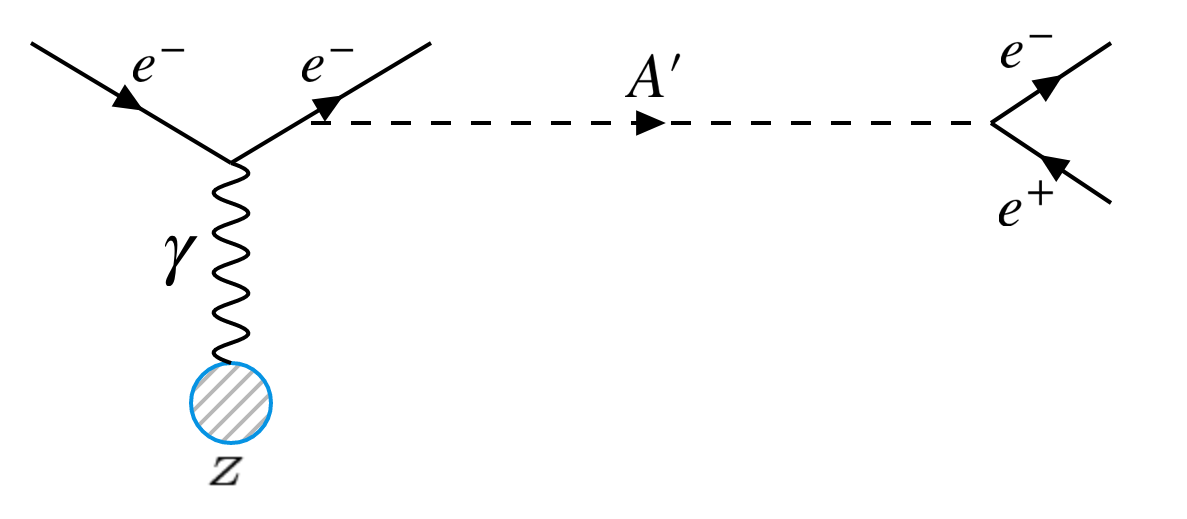
\includegraphics[width=14.5cm]{thesis_figures/VISIBLE.png}
\caption{Visible mode }
\label{fig:Visible_feynman}
\end{figure}

\begin{figure}[t!]
\centering
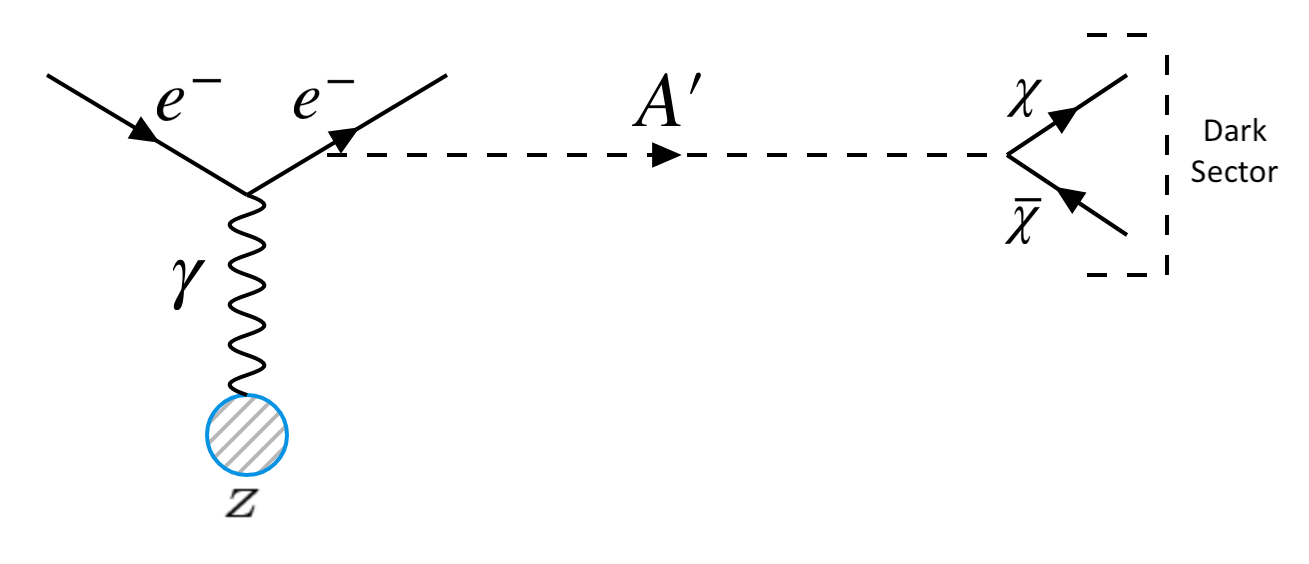
\includegraphics[width=15cm]{thesis_figures/INVISIBLE.png}
\caption{Invisible mode }
\label{fig:Invisible_feynman}
\end{figure}
Clearly from eq.(\ref{eq:Lagrangian}) there are two possibilities for the detection of $A'$. It can be either observed via its decay to SM particles which is called the \textit{visible mode} (fig.(\ref{fig:Visible_feynman})) or via its decay to light DM particles known as the \textit{invisible mode} (fig.(\ref{fig:Invisible_feynman})). In the visible mode we assume that $A'$ is one of the lightest states in the dark sector, then it is fair to believe that it would mainly decay to SM leptons. Such an interaction is described by the Lagrangian ${\cal L}_{int} = \epsilon e A'_{\mu} J^{\mu}_{em}$ where $J^{\mu}_{em}$ is the electromagnetic current and $e$ is the electromagnetic coupling. Such a decay would assume the $A'$ to have a sub-GeV mass and $\epsilon \ll 1 $. It also allows for an opportunity to set up an experiment for this particular mode since we will directly observe an excess of leptons in the final state. On the other hand for the invisible mode we assume that $A'$ is not the lightest state and there exists some other state $\chi$ with a lower mass, such that $A'\rightarrow \chi \overline{\chi}$ is a possibility. Such an event can also be probed with a so called missing energy experiment where the produced $A'$ or $\chi$ carries away some of the energy and is not detected.

The production and detection mechanisms discussed offer us the basic ingredients needed to set up an experiment for the detection of $A'$. One of the simpler layouts for such an experiment is an electron beam dump experiment. NA64 falls in this category, the setup of which is discussed in the next chapter.
\begin{figure}[t!]
\centering
  \begin{minipage}[t]{.45\textwidth}
    \centering
    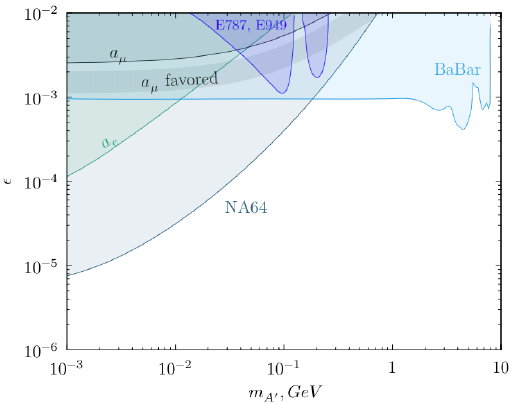
\includegraphics[width=\textwidth]{thesis_figures/exclusion_invisible.png}
    \caption{Current limits for invisible mode for 90\% C.L. exclusion region in the ($m_{A'},\epsilon$) plane ~\cite{2019EPJWC.21206005K}.}
    \label{fig:exclusion_invisible}
  \end{minipage}
  \hfill
  \begin{minipage}[t]{.45\textwidth}
    \centering
    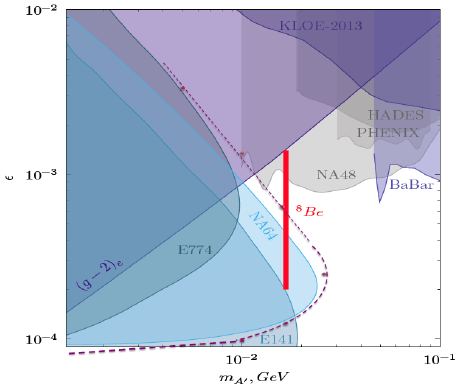
\includegraphics[width=\linewidth]{thesis_figures/exclusion_visible_latest.png}
    \caption{Current limits for invisible mode for 90\% C.L. exclusion region in the ($m_{A'},\epsilon$) plane. The blue plane is with 2017 data and the dotted line is with 2017+2018 data for NA64. The red line is the region that might explain the X17 boson~\cite{2019EPJWC.21206005K}.}
    \label{fig:exclusion_visible}
  \end{minipage}
\end{figure}


%%% Local Variables:
%%% mode: latex
%%% TeX-master: "mythesis"
%%% End:

% !TEX root = mythesis.tex

%==============================================================================
\chapter{NA64 Experimental Setup}
\label{sec:setup}
%==============================================================================
\begin{figure}[h!]
\centering
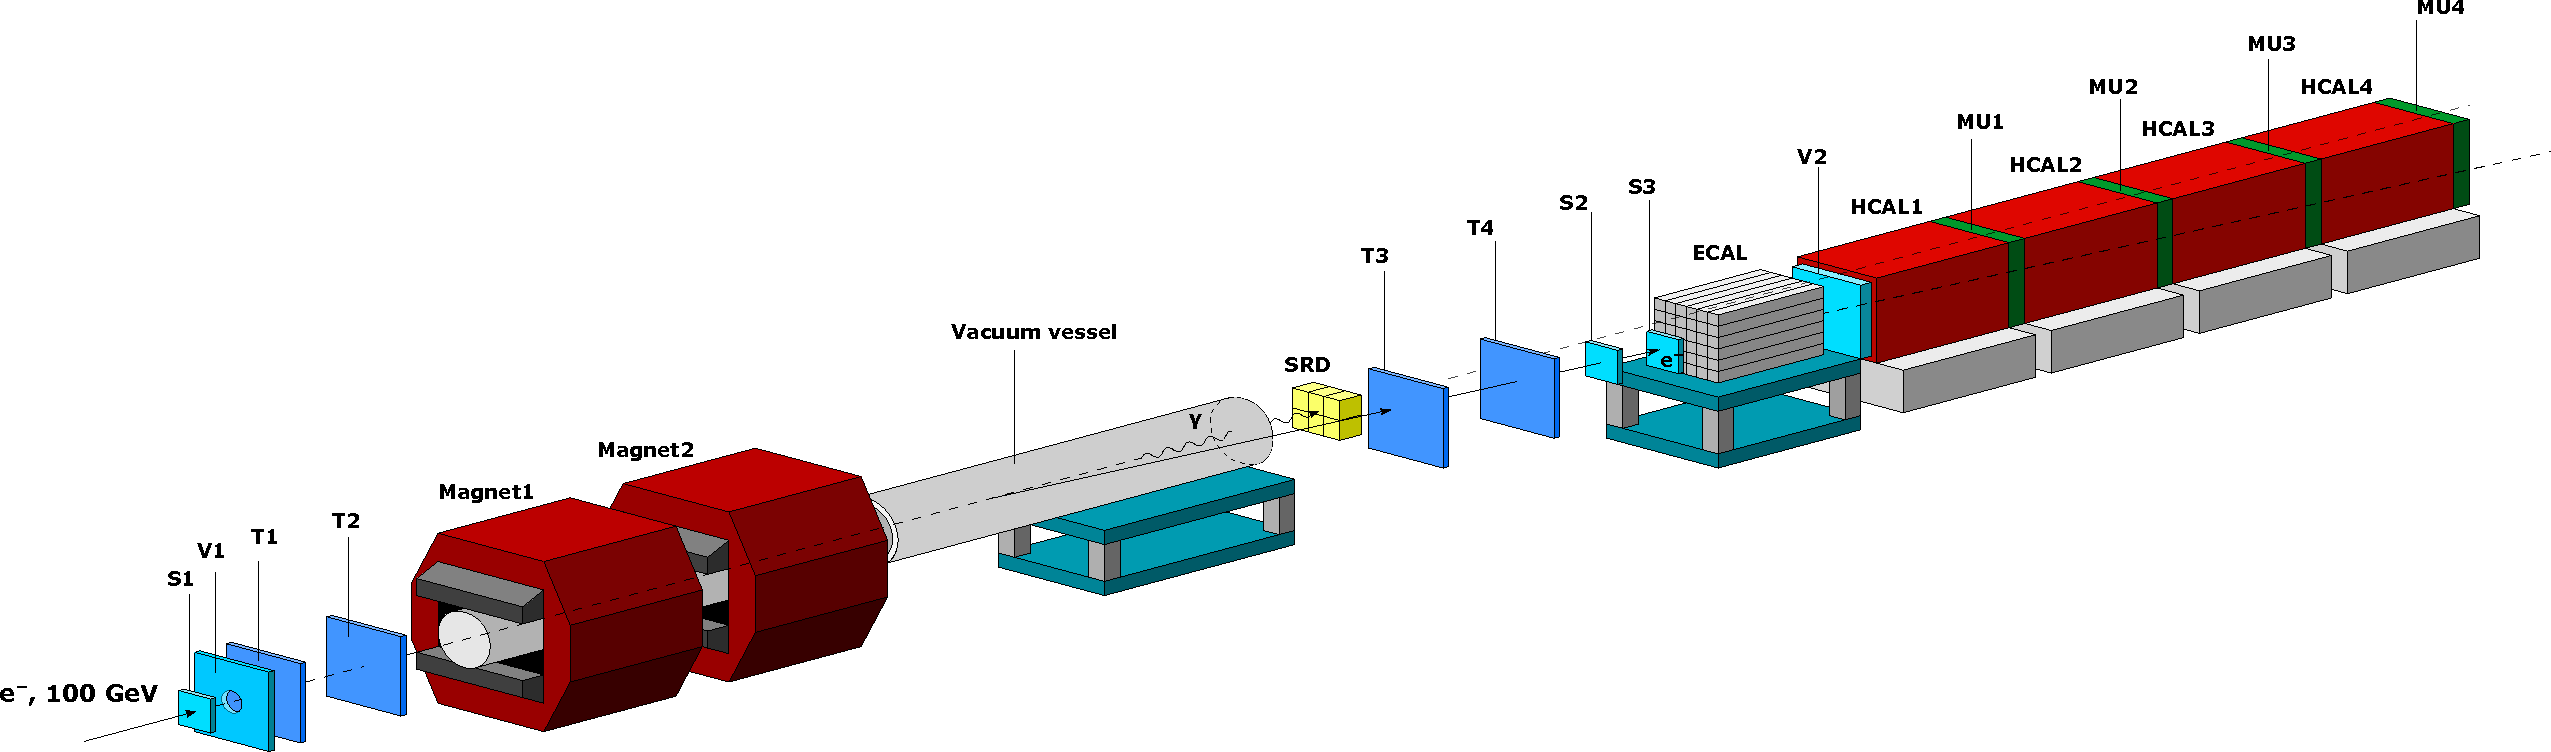
\includegraphics[width=\textwidth]{thesis_figures/Invisible_3d_setup.png}
\caption{Invisible mode setup~\cite{Banerjee:2016tad}}
\label{fig:Invisible_mode_setup}
\end{figure}

NA64 is a beam dump fixed-target experiment located at the H4 beam line of the Super Proton Synchrotron (SPS) at CERN. The objective of the detector is to look for rare dark matter candidates, primarily Dark Photons $A'$. $A'$ is supposed to be emitted via a process similar to bremsstrahlung $e^-Z\rightarrow e^- Z A'$. The experiment is not a permanent fixture and has been in operation since March, 2016. Since it's approval the setup has taken data a total of four times which included a two week test run in 2016 and four weeks of data taking each in 2016, 2017 and 2018. Each year the setup has slightly varied to account for different beam energies and expected background.

The SPS provides a primary proton beam of $400~\mathrm{GeV/c}$ with $\simeq 10^{12}$ protons per spill which is then converted to electrons by incidence on a beryllium target. The $e^-$ beam is in the momentum range $50-150~\mathrm{GeV/c}$ with a maximal intensity $\simeq 10^{7}$ per SPS spill of 4.8s. The provided high-energy $e^-$ beam with the large luminosity was needed since the $A'$ couples very weakly to the SM. The beam is then characterized by passing it through scintillators (S1-S3),veto ($V_1$), two dipole magnets with an integral magnetic field of $\simeq 7~\mathrm{Tm}$ and trackers (MM-section(\ref{sec:MM}), GEM-section(\ref{sec:GEM}) contained in tracking stations (T1-T4) which measure the $e^-$ beam momenta to a 1\% precision~\cite{article_beam_purity}. Additionally the combination of magnets followed by a 15m long vacuum vessel and a PbSc synchrotron radiation detector (SRD) acted as a filter to reject low energy electrons and hadrons that might be present in the beam and would contribute to the overall background. They were separated by putting a cut on the amount of synchrotron radiation energy deposited by the respective particle~\cite{Gninenko:2013rka}. The beam is then allowed to hit the electromagnetic calorimeter (ECAL) which acts as an active target. The ECAL consisted of 6x6 Shashlik-type modules each with 40 radiation lengths ($\mathrm{X_0}$) of which the initial 4$\mathrm{X_0}$ is employed as a separate preshower(PS) detector. The ECAL had a resolution of $\delta E_{ECAL}/E_{ECAL} \simeq 0.1 \sqrt{E_{ECAL}[\text{GeV}]}$~\cite{Banerjee:2016tad}.
The combined information achieved by studying the shower and the SRD signal helped in suppressing the hadron contamination in the beam to a remaining fraction of $ \lesssim 10^{-6}$~\cite{Depero:2017mrr}. A combination of Veto($V_2$) and hadronic calorimeter(HCAL) is situated downstream of the ECAL. They serve as a veto against muons, neutrals like high energy photons or hadrons produced in the target ECAL. The HCAL consisted of four modules ($\text{HCAL}_{1-4}$) separated by muon counters ($MU_{1-4}$) and were slightly shifted along the beam with each module consisting of 3x3 cells adding up to a total of $\simeq$30 nuclear interaction length ($\lambda_{int}$). The HCAL had a resolution of $\delta E_{HCAL}/E_{HCAL} \simeq 0.6 \sqrt{E_{HCAL}[\text{GeV}]}$~\cite{Banerjee:2016tad}.

\begin{figure}[t!]
\centering
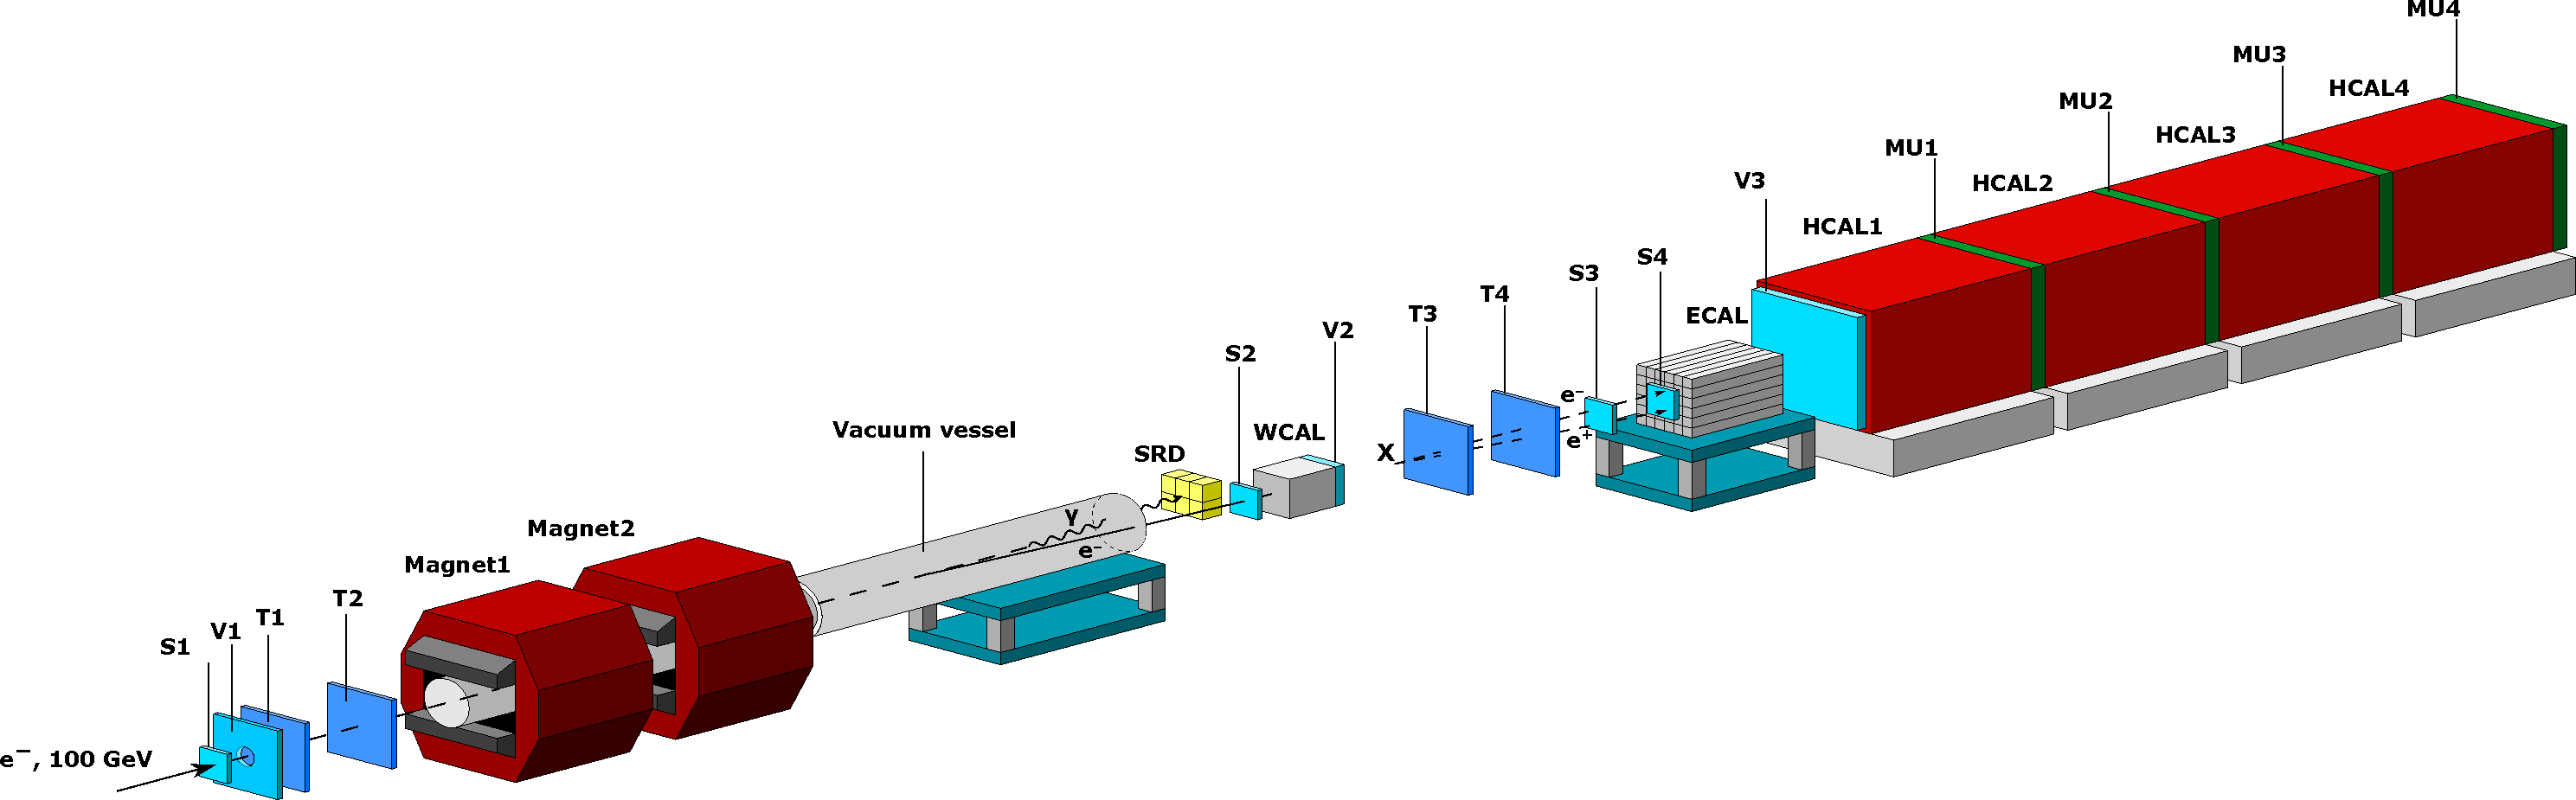
\includegraphics[width=\textwidth]{thesis_figures/Visible_3d_setup.png}
\caption{Visible mode setup 2017~\cite{Banerjee_2018}}
\label{fig:Visible_mode_setup}
\end{figure}

\begin{figure}[t!]
\centering
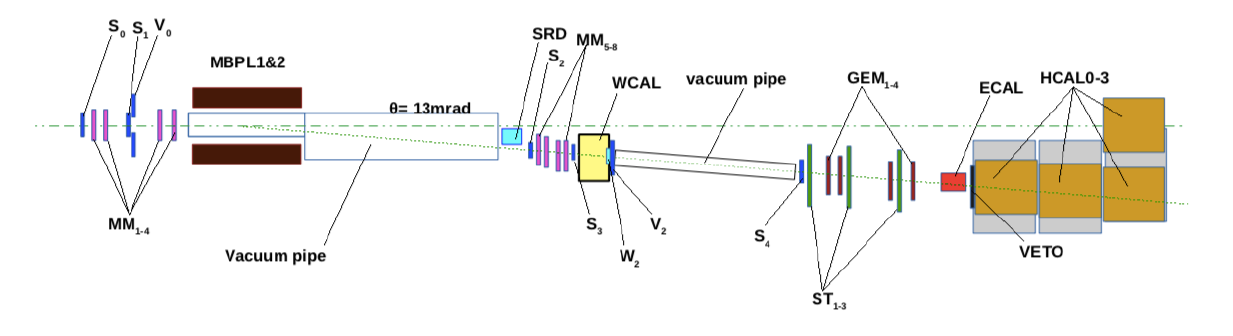
\includegraphics[width=\textwidth]{thesis_figures/visible_mode_newest.png}
\caption{Visible mode setup 2018-top view~\cite{Gninenko:2677228}}
\label{fig:Visible_mode_setup_side}
\end{figure}

The above setup works well for the \textit{invisible mode}($10^{-4} \lesssim \epsilon \lesssim 10^{-3}$, $m_{A'} \lesssim 1 \text{GeV}$) but requires modification for the search of $A'(X)$ in the \textit{visible mode}($10^{-4} \lesssim \epsilon \lesssim 10^{-3}$, $m_{A'} \lesssim 100 \text{MeV}$). To search for the visible decays a short tungsten calorimeter (WCAL) and a veto ($V_2$) were added right after the vacuum pipe and before the second set of tracking detectors (fig.(\ref{fig:Visible_mode_setup})). The size of the WCAL was selected so that the leakage of particles is small and the sensitivity to short lifetimes is maximized. The distance between the WCAL and the ECAL for the visible mode searches was slightly varied(2.5m->5.6m) between 2017 and 2018 which allowed for the installation of a 3.1m long vacuum tube to create better spacing between the ECAL and WCAL for a better angular resolution to increase the sensitivity to X17 bosons~\cite{Banerjee_2018}. A WCAL catcher was also installed in 2018 to prevent any leakage. Additionally the beam momentum was increased from 100GeV to 150 GeV in 2018 and one of the tracking station consisting of two MicroMegas (MM) was also shifted upstream of the WCAL. Counter ($W_2$) and straw detectors ($\text{ST}_{1-3}$) were also tested during the 2018 beam period(fig.(\ref{fig:Visible_mode_setup_side})). Both \textit{invisible} and \textit{visible} mode setups were also used to look for rare SM events that involve a photon decaying to a dimuon pair via bremsstrahlung $e^-Z\rightarrow e^-Z\gamma;\gamma\rightarrow \mu^{+} \mu^{-} $. Comparing these rare events, which were obtained from real data, to our Monte Carlo(MC) simulated sample helped in estimating the validity and efficiency of our MC simulation~\cite{Gninenko:2677228}.

In summary, NA64 tries to estimate and tag the beam $e^-s$ using a combination of trackers, SRD and ECAL/WCAL, uses the said ECAL/WCAL as an active target and then collects the residue of the interaction in the downstream HCAL/ECAL+HCAL. It also utilizes the hard bremsstrahlung photon to dimuon conversion as a measuring stick for the reliability of the MC simulations. The reactions of interest were attempted to be observed with a combination of hardware and software triggers depending on the expected signature of the decay mode for $A'$.

\textbf{Invisible Mode:}
$A'\rightarrow \chi \overline{\chi}$ signature:
\begin{flalign*}
  Beam(p\simeq 100~\text{GeV}),\\
  E_{ECAL+PS}(< 100~\text{GeV}),\\
  V_2(< E^{th}_{V}\simeq 1~\text{MIP}),\\
  E_{HCAL}(< E^{th}_{HCAL}\simeq 1~\text{GeV}).
\end{flalign*}

\textbf{Visible Mode:}
$A'\rightarrow e^+ e^-$ signature:
\begin{flalign*}
  Beam(p\simeq 150~\text{GeV}), \\
  E_{WCAL}(< 150~\text{GeV}), \\
  E_{WCAL+ECAL+PS}(\simeq 150~\text{GeV}), \\
  V_2(> E^{th}_{V}\simeq 1~\text{MIP}), \\
  V_3(< E^{th}_{V}), \\
  E_{HCAL}(< E^{th}_{HCAL}\simeq 1~\text{GeV}).
\end{flalign*}







%%% Local Variables:
%%% mode: latex
%%% TeX-master: "mythesis"
%%% End:

% !TEX root = mythesis.tex

%==============================================================================
\chapter{Neutrino Analysis $60^\circ < \theta < 75^\circ$}
\label{sec:DGL}
%==============================================================================
This chapter gives a brief summary of the neutrino search performed for the zenith range $60^\circ < \theta < 75^\circ$. The neutrino search is separated in different angular range to maximise the performance of the detector array in this case the SD for the search. The chapter aims to cover the expected signature in terms of measurable quantities in the Pierre Auger Observatory for the particular angular range, the neutrino simulation used to develop the analysis, the reconstruction chain used along with the quality cuts used for such an analysis. Further, the quality cuts are analysed in more detail especially in the context of improving the capability of the search by the usage of MoPS and ToTd. In the end the improvements to both the diffused and point source neutrino searches with the new triggers are quantified.


\section{SD Neutrino signature $60^{\circ} < \theta < 75^{\circ}$}
\label{sec:sig_DGL}

The strategy and method to detect neutrino showers in this angular range with the SD remains the same as mentioned before i.e to try detecting showers that develop late and have more electromagnetic or "young" shower front at ground. In terms of signal in the SD array the young shower is expected to be spread over a longer time period typically hundreds of nanoseconds and have a lower maximum peak compared to signal induced by older showers which are spread over tens of nanoseconds and have a higher maximum peak. A comparison of the difference between the induced SD signal from a young and old shower arriving from the same zenith angle is presented in fig. ~\ref{}. However, such differences in signals and the ability of the SD to differentiate between a neutrino induced and a proton/ heavy nuclei induced shower disappears for vertical showers($\Theta < 60^{\circ}$). For vertical showers a cosmic ray induced shower does not have enough time to develop because of the limited thickness of the atmosphere. At these zenith angles a high energy CR induced EAS can mimic the expected young shower signature of a neutrino induced EAS at ground. Thus, currently the neutrino searches at the Pierre Auger Observatory are limited to zenith angles above $60^\circ$ where it is much easier to separate a neutrino induced EAS from a CR induced EAS. Since we are also searching for young showers which have not fully developed till they are detected at ground, reconstructed energy cannot be used as a discrimination criterion.      

To select the longer signals in the SD one of the variables that was used in erstwhile neutrino searches is the fraction of ToT-T2 triggered signals in the recorded event. As mentioned in the previous chapter this trigger is tuned to select broader signals which for an inclined shower is evidence of a young shower. For the search presented in this thesis along with the ToT-T2, the ToTd and MoPS are also used. Both ToTd and MoPS as mentioned in sec.~\ref{} help further increase the selection efficiency for broader signals by reducing the impact of low energy muons. These muons which form the majority of the background at low zenith angles of the selected search range. Thus, these triggers are impactful in increasing the separation power for low energy($\leq$ 1 EeV) neutrino showers. Another important variable which is used to judge the width of the signals is Area Over Peak (AoP). The AoP is defined as the ratio of the integrated signal of the station over the biggest value or peak of the signal. The AoP is calibrated in such a way that narrow/ old shower signals have AoP ~ 1 while broad/old shower signals have AoP $\geqslant $ 1. 



\section{Neutrino Simulations}
\label{sec:sim_DGL}
To characterise the neutrino search ability of the Pierre Auger Observatory Monte Carlo simulations of EASs induced by UHE$\nu$s are required. There are six possible neutrino interaction chanels due to the three possible neutrino flavors with each having two possible channels(CC or NC). However, for simulations these are envisioned to be characterised by just two sets of simulations. For the NC channel since the EAS induced by three neutrino flavors has the exact same signature for our detector only $\nu_e$ NC simulations were performed to estimate the NC contribution of all the three flavors to the final exposure. 

For the CC interactions in the case of $\nu_{\mu}$ the resulting high energy muon has a high probability of evading detection. This is very similar to the NC interaction where the resultant secondary neutrino also carries approximately 80\% of the primary energy. Thus, after taking into account the appropriate crossection, in principle the NC simulations can be used to also estimate the contribution of $\nu_{\mu}$ CC channel.  

In the case of $\nu_{\tau}$ CC interactions where the resulting $\tau$ especially at higher energies($\geq $EeV) can decay and also initiate a secondary shower resulting in a "double bang" like signature in the Observatory. In the context of this thesis such signatures are not accounted for and the $\nu_{\tau}$ CC interaction is treated in the same way as the $\nu_{\mu}$ CC interaction resulting in a possible underestimation of the Observatory to $\nu_{\tau}$ events. A future $\nu_{\tau}$ simulation library is currently being prepared by the Pierre Auger Collaboration Monte Carlo task and could help extend this analysis in the future.

Thus, in summary $\nu_e$ CC and NC simulations can be considered to be good approximations to estimate the contributions of all the other channels to the overall exposure of the Observatory. The simulations were produced in two parts by the Pierre Auger Collaboration Monte Carlo task based on the GAP note ~\ref{}. The first part entails the simulation of the $\nu$ induced EAS in the atmosphere and the second consists of simulating the appropriate detector response for the corresponding shower. 

\subsection{Atmospheric Shower simulations}
\label{subsec:sim_EAS}
The first part included using CORSIKA~\ref{} to generate the EAS initiated by a $\nu$ primary. This involves simulating the primary neutrino-nucleon interaction which is performed in CORSIKA using the HERWIG code. Further options such as CHARM to track charm secondaries are not used. Also since only $\nu_e$ simulations are simulated, the TAULEP option which handles $\nu_{\tau}$ and $\overline{\nu_{\tau}}$ is also not used. The systematic uncertainties related to the primary interaction estimator is discussed later in section~\ref{}. CORSIKA further tracks the primary interaction products as they travel in the atmosphere towards the ground constituting the air shower. CORSIKA offers a wide variety of choice regarding selecting the hadronic interaction model. For the simulations used in this study separate high and low energy hadronic interaction models were used. For energies higher than 200 GeV three high energy hadronic models QGSJETT~\cite{}, SYBILL~\cite{} and EPOS-LHC~\cite{} were compared. The results of the comparison are mentioned in detail in Appendix~\ref{}. Since the differences between the models are not that significant for the neutrino analysis ....dash..... was chosen as the high energy interaction model. For lower energies FLUKA~\cite{} was chosen. The systematic uncertainities arising from different models are discussed in section~\ref{}.  

To account for the curvature of the Earth which is especially important for the zenith angles studied, the EGS4~\ref{} Monte-Carlo method is chosen to simulate the electromagnetic component of the shower. The analytical NKG~\ref{} method which is also available but is not used for these simulations since it vastly underestimates the maximum of the electromagnetic component due to the fact it does not account for a curved atmosphere. GDAS Malargue October atmospheric profile is chosen for the simulations and the magnetic field components are taken to be the default values at the Malargue site ($B_x = 19.52\mu T$ and $B_z = -14.17\mu T$). 

Further, since the computing times taken for shower simulations scale roughly with the primary energy, for primary energies > $10^{16}$eV these times become extremely long. Though parallel computing provides a viable solution, the technique of "thin sampling" or thinning~\cite{} offers an alternate way to reduce the computation times while simultaneously saving wastage of resources. The thinning algorithm is applied to all particles below the adjustable fraction of the primary energy which emerge from an interaction. Only one of these particles is followed ,and a proper weight is assigned to this particle to account for the untracked ones which are dropped based on the thinning level($\epsilon_{th} = E/E_0$). Additional improvements ~\cite{} which reduce the statistical fluctuation of particle densities far from the shower core using a maximum limitation of weights and reduction of number of particles close to the shower core where the detectors anyway have a high chance of saturation are also used as a part of thinning algorithm in CORSIKA. A thinning value of $10{-6}$ is used for the simulations in this study. An example of the CORSIKA input file used by the MC task to produce the simulated showers is shown below:

\todo{Add The CORSIKA steer file}

The simulations were performed using the GRID technology~\cite{}. Both CC and NC showers were simulated for fixed energy steps of log(E/eV) = 0.5 in the range $10^{17}-10^{20.5}$eV. The number of simulated showers was varied depending on the Energy, atmospheric depth of interaction and the injected zenith angle. More showers were simulated at lower energies and the energy dependent numbers are tabulated in table~\ref{}. Further, for both the interaction channels within the zenith angle range $60^{\circ}-70^{\circ}$ the neutrinos were forced to interact at fixed atmospheric depths in steps of 100 g cm$^{-2}$. The injection points both close to the ground where a neutrino shower might have a lower trigger efficiency and close to the top of the atmosphere where a neutrino induced shower might mimic one induced by a proton are rejected for the simulations. The azimuthal angle is left free and can take any value between 0$^{\circ}$ and 360$^{\circ}$. The simulated depths for each zenith angle bin are summarised in table~\ref{}. 

Based on (E,$\theta_{MC}$,X) bin the number of CORSIKA showers simulated vary. Higher values were chosen for lower energies to increase the statistics since at these energies the simulated shower has a higher chance of not being detected be the detector.  

After the simulation is completed CORSIKA produces a normal particle output file which contains information about the surviving particles on the ground level which is set based on the detector elevation. The file contains the relevant information such as energy, momentum, timing all segregated for each particle based on its Particle Data Group Code~\cite{}. It also produces a ".long" file which contains longitudinal distribution of various particle numbers along with the energy deposited which is relevant for fluorescence telescope based analyses. For this work the normal particle output files were used for further processing to simulate a response in the Pierre Auger Observatory SD.

\subsection{Surface Detector Response}
\label{subsec:sim_SD_resp}

The next step required to complete the $\nu$-induced shower simulation is to generate an appropriate detector response in the SD array for each simulated atmospheric shower. This is done using the Offline framework. The framework can read in the CORSIKA output files, undo the applied thinning, simulate the Cherenkov light which will be produced as the particles travel through the WCDs and then also mimic the corresponding WCD electronics outputting the trigger and event information for each simulated shower akin to how real showers are measured at the Observatory. Each step is performed using special modules. The module sequence used to simulate the detector response for $\nu$-induced showers in this thesis is given below: 

\todo{Add The module sequence}


The \textit{EventFileReaderOG} reads in the CORSIKA output file. The following steps are performed assuming an "ideal" SD array with every station operational and fully efficient within the design limts. The steps are also repeated for an individual shower between 5- 30 times depending on the primary energy to further increase the statistics for each (E,$\theta$,X) bin. The first module is the EventGeneratorOG sets the core position, time and event ID for Monte Carlo events. In this analysis similar to ~\cite{} the core position is only allowed to be randomised over a 5 x 5 km$^2$ area around a fixed station at the center of the array. This allows an in depth study of how core position could impact the reconstruction which is discussed later. In the next step the \textit{CachedShowerRegeneratorOG} reads in the list of the shower particles and unthins each particle injecting a set of new particles based on its unique weight~\cite{}. It can then create a list of particles for each SD station which is then passed to the next module \textit{G4TankSimulatorOG}. G4TankSimulatorOG uses Geant4~\cite{} to simulate the particle trajectories in the WCD and the corresponding Cherenkov light produced by these particles. It also handles all the possible absorption and reflection the light can suffer before it is measured by the PMT. Following this the \textit{} simulates the detector calibration constants described in section~\ref{} and the \textit{SdPMTSimulatorOG} takes in the information from the tank simulator and simulates a corresponding PMT signal(trace). \textit{SdFilterFADCSimulatorMTU} and \textit{SdBaselineSimulatorOG} further simulate the processing of the PMT signal by the electronics at each station with the first applying the filter response and the FADC sampling and the second adding baseline and simulated noise to these traces. 

The next two modules decide whether the simulated event fulfills the heirarichal trigger system of the Observatory explained in section~\ref{}. \textit{TankTriggerSimulatorOG} checks if the signal fulfills the local station criteria i.e T1 and T2 condition after which the \textit{CentralTriggerSimulatorXb} further combines all the station which fulfil the T2 criteria to form the T3 simulating the task performed by CDAS for real data. The \textit{CentralTriggerEventBuilderOG} and \textit{EventBuilderOG} then facilitate the transfer of events passing the T3 criteria from the simulation container class to the event class with the last module \textit{EventFileExporterOG} responsible for exporting all the processed showers now with the applied detector response in a file which can be further used for further reconstruction.  


\section{Shower Reconstruction}
\label{sec:reco}

The event reconstruction is a necessary step before any further analysis can be performed. This procedure is developed first for neutrino simulations to enhance their identification efficiency and then applied to real measured data for both estimating the possible background for a neutrino like events and for the final search for neutrinos at the Observatory. Shower reconstruction is also performed within the Offline framework with a module sequence that contains a combination of some standard reconstruction modules and some specific modules developed for neutrino identification in GAP note~\cite{}. The reconstruction is again performed with the help of the MC task on the GRID framework based on the particular reconstruction chain developed for neutrinos. The Module sequence used to reconstruct simulated neutrino showers is given below:

\todo{Reco modulesequence}

The sequence remains similar to the one used in~\cite{} apart from the iterative development performed by the Offline developers over the years. For data reconstruction the \textit{SdMonteCarloEventSelectorOG} is omitted from the sequence. The chain can be subdivided to three main parts which are "event reading and pre-selection," "angular reconstruction" and "posterior selection and export" which are discussed in the next few sections.

\subsection{Event reading and pre-selection}
\label{subsec:reco_presel}

The first module in this part of the reconstruction is again the \textit{EventFileReaderOG} which depending on the input format can parse the file. In the reconstruction sequence it is used to read in either the detector response simulated file for simulations or the measurement files obtained from the SD. The \textit{EventCheckerOG} further checks if the stations in each read event have proper timing information. After this point the FADC traces are processed with various modules to covert them to VEM units. The \textit{SdGainRatioCorrectorKG} corrects for the gain ratio for the electronics followed by \textit{TriggerTimeCorrection} which further corrects for differences in electronics especially related to timing for data over the course of its operation. The \textit{SdStationCheckerOG} further checks the station quality and appropriately sets silent stations if they do not contribute to the final trigger formation. After this point the \textit{SdHistogramFitterKG}, \textit{SdBaselineFinderKG} and \textit{SdTraceCalibratorOG} which get the calibration constants from the calibration traces, fit the baseline and the convert the traces to VEM units respectively. Further modules \textit{SdStationPositionCorrection} corrects the positional differences that might arise due to faulty GPSs which is important for correct timing information, \textit{SdBadStationRejectorKG} sets known bad stations in the array to be inoperational and the \textit{SdSignalRecoveryKLT} which tries to recover signals from the saturated PMTs if any by looking at the undershoot value~\cite{}. An extra module \textit{SdPMTQualityCheckerKG} is also used in the case of data reconstruction to estimate the quality of the detector.

The next three modules are used to fine tune the selection of signals and later events to improve the both the quality of simulated and measured data to increase the efficiency of neutrino detection. The first one is the \textit{SdEventSelectorOG} which applies a basic SD event selection which is also used in other analyses. The module sets conditions based on T4, T5 and other station based parameters if appropriate. The different operations performed by the module are as follows:

\begin{description}
  \item $\bullet$~\textbf{Bottom-up Selection:} This selection helps in deciding the non-participating stations if the stations are not compatible with a planar shower front propagating at the speed of light hypothesis~\cite{}. Such stations can arise due to random noise in the array or due to random coincidences between non-air shower events with air shower events. The selection requires a minimum of three stations which fit the planar front of the shower within lenient time tolerances. It also removes isolated stations by checking the distances to nearest neighbors. Though, the selection is applied, it is not very effective for inclined showers(>$60^{\circ}$) since the showers above these angles are not geometrically compact. Thus, this selection is supplemented with an extra top-down selection implemented in \textit{SdTopDownSignalSelectorUGR} which is discussed later. 
  \item $\bullet$~\textbf{T4 and T5 trigger:} The module also calculates the T4 and T5 criteria discussed in sec.~\ref{}. It also then further discards events if they do not fulfill these criteria. In this study the T4 criteria was not required but a stringent 6T5 criteria was required for the selection. 
  \item $\bullet$~\textbf{Lightning Rejection:} The lightning events can be detected in the SD stations by looking for oscillatory signal in the FADC trace of all three PMTs~\cite{}. For this analysis if any lightning like signal is detected in any one of the stations the whole event is rejected from the analysis. 
  \item $\bullet$~\textbf{ToTd and MoPs trigger:} The module can also silence particular triggers before applying the selection. This feature is used to produce two sets of reconstruction files one with the triggers turned off and one with them turned on. This can impact the number of events fulfilling the 6T5 conditions and thus the overall number of events which can be seen later.    
\end{description}

The \textit{MonteCarloEventSelectorOG} further removes stations with distance in shower plane coordinates smaller than the inner radius used in the CORSIKA simulations. It also removes dense stations i.e virtual stations which are sometimes used for MC studies since these are not representative of the regular SD array. 

The \textit{SdTopDownSignalSelectorUGR} is a module developed specially to carry out a top-down selection and accidental signal rejection for neutrino like events. A summarised overview of what this module aims to accomplish is given next with a detailed description of the module already published in ~\cite{}. The Top-down procedure is applicable for both the simulations and measured data whereas the accidental signal treatment is only applied for measure data. The procedure is based on~\cite{} and ~\cite{}. Top-down selection requires a minimal of three station with the shower front time tolerance compatibility dependent on the zenith angle. If the fit does not converge stations are successively removed and re-tested until a satisfactory fit is achieved. At the end of the procedure stations which do not contribute to the final fit are rejected while the others are marked as candidate stations. Further the Top-Down procedure also takes into account the individual traces and uses the shape for 3-fold topologies. It also rejects isolated signals akin to the Bottom-up selection but with larger tolerances to account for the wider footprint of inclined events. The module also applies an accidental signal rejection procedure before the top-down procedure is applied to account for the atmospheric muon background. The atmospheric muons and also local showers can either trigger isolated stations or even real event stations affecting the start times and in turn the zenith angle reconstruction. This miss-reconstruction can either cause problems with the fitting of the top-down procedure and can also lead non-neutrino like or background events pass the analysis cuts affecting the overall neutrino detection efficiency. The module discards stations with total signals below 3 VEM which rejects the muonic background which typically peaks at 1 VEM. The discarding procedure is implemented only till the minimal number of stations present in the event are below 6. 


\subsection{Angular Reconstruction}
\label{subsec:reco_presel}

The angular reconstruction forms the basis for neutrino detection using the SD especially since for inclined neutrinos the energy reconstruction algorithms typically used for cosmic rays at the Pierre Auger Observatory become unreliable. The angular reconstruction is performed by the \textit{SdPlaneFitOG} and \textit{LDFFinderKG}. The energy reconstruction using the SD is either typically done using the \textit{LDFFinderKG} which fits a lateral distribution function to the SD signal based on the NKG approximation. The NKG approximation is typically inaccurate for inclined showers above a zenith of $60^{\circ}$ thus alternate methods based on muon maps are used for inclined showers. These also fail for neutrino induced showers usually having a large electromagnetic component. Thus, without a reliable energy reconstruction angular reconstruction becomes vital for neutrino induced shower detection at the SD. 

The angular reconstruction procedure uses the timing information from the stations to fit either a plane or a spherical shower front. The axis of shower $a$ is initially assumed to intersect the ground at some time using a signal weighted barycenter $x_b$ and bary-time $t_b$ of selected stations located at $x_i$ with start time $t_i$ given by :




The choice of the weights taken as $\sqrt{S} $ with $S$ being the signal of the stations has been previously evaluated using Monte-Carlo studies~\cite{} to give the best results. The barycenter also serves as the first estimate of impact position of \textit{shower core} at ground but is later estimated more accurately. The shower core is assumed to be moving in the $-a$ direction. Under the plane-front assumption the particles in the shower front move in a plane perpendicular to the shower axis($shower plane$) with the same speed as the core of the shower which is the speed of light c, the time t(x) when the shower plane passes through some chosen point
x (e.g. a station on the ground) can be inferred through a simple projection onto the shower axis as,


Assuming a minimal change in altitude which is true for SD location and precise knowledge of station locations the deviations in estimating the geometrical shower parameters can be due to the uncertainity of the observed start times $\sigma_t$. Thus, the following function needs to be minimised to fit the model for the measured signal start times 


The start time variance needs to be modified for the new triggers and has been taken from~\cite{}. Replacing the axis with $a =(u,v,w)$ and the station coordinates with $x = (x,y)$ (ignoring altitude z). Adding the constraint $u^2 + v^2 + w^2 = 1$ the $chi^2$ can be easily solved. The solution only fails if the stations used while fitting have a linear dependence(three stations in a line) but for higher station multiplicity this is highly improbable especially for the theta range explored for the DGL channel. For more inclined events different solutions to the zenith estimation are used~\cite{}. 
 
Another shower front estimation technique based on a curved shower front approximation is also used to fit the measured stations~\cite{}. The reconstruction assumes the shower development starting at time $t_o$ from a point of origin $x_o$ propagating toward the ground as a concentrically expanding sphere with the speed of light, $c$. The arrival time can thus be estimated as:


As can be seen by the equation, the spherical fit is decoupled from any prior knowledge of the shower core or the shower axis. It is only dependent on the point of origin. Quantities such as shower axis can be determined later when the impact point has been estimated as $x_o -x_c/ x_o-x_c$. The expected solid angle differences between the two fits are of the order of half a degree. The curvature shower front fit is only used for station multiplicities greater than five. This is so because for lower station multiplicities the degrees of freedom are not enough to solve for the shower-front curvature(R-$\infty$). 


\subsection{Posterior selection and Export}
\label{subsec:reco_possel}

The last part of the shower reconstruction chain includes the application of the \textit{SdEventPosteriorSelectorOG} module which computes the 6T5 \textit{posterior} trigger differing from the 6T5 criteria mentioned earlier. The 6T5 posterior requires the 6 stations in the first crown from the nearest station to the reconstructed shower axis to be active or alive during the event. The events which do not pass this criterion are rejected. The last module \textit{RecDataWriterNG} exports all the relevant information to ADST~\cite{} files. In case of reconstructed simulations both the simulated and reconstructed information is stored while for measured data only the reconstructed information is stored.


\section{Reconstructed $\nu$ simulations}
\label{sec:reco_possel}
This section includes some sanity check to check and verify the quality of the $\nu$ simulations. Fig shows the  Efficiency of the reconstructed showers as a function of the zenith angle and the slant depth. The next figure shows the frequency of reconstructed events based on the core position. The non-uniform distribution with the minimal events for core positions close to the stations can be explained due to two reasons. The first being the removal of stations if the PMTs for the particular station is saturated. This saturation can occur for stations very close to the core. The second reason  



\section{$\nu$ selection}
\label{sec:nu_sel}
This section tries to describe the decisions made to select $\nu$ induced air showers. The selection is optimised and evaluated on the above-mentioned neutrino simulations and a part of measured data used as an estimate for the expected background. Since a \textit{blind search} strategy is envisioned for the search. The rest of the measured data forms the \textit{search sample} and will be used to look for neutrino like events during \textit{unblinding}. 
In the first part the selection used to select $\nu$ showers is described in more details. The selection consists of some pre-selection cuts applied to enhance the reconstruction quality of the selected events followed by a Fisher Linear Discriminant~\cite{} based on experimental observables which is the main criteria of differentiation between a $\nu$ induced air shower and background.  
In the second part the performance of the selection is further evaluated based on temporal changes such as aging in the surface detector along and the neutrino detection efficiency is quantified. Comparison to previously used selection are also discussed especially in the context of the performance improvements achieved by using new triggers for neutrino detection.

\subsection{Samples Used}
\label{subsec:nu_sel_samp}



\begin{figure}[t!]
\centering
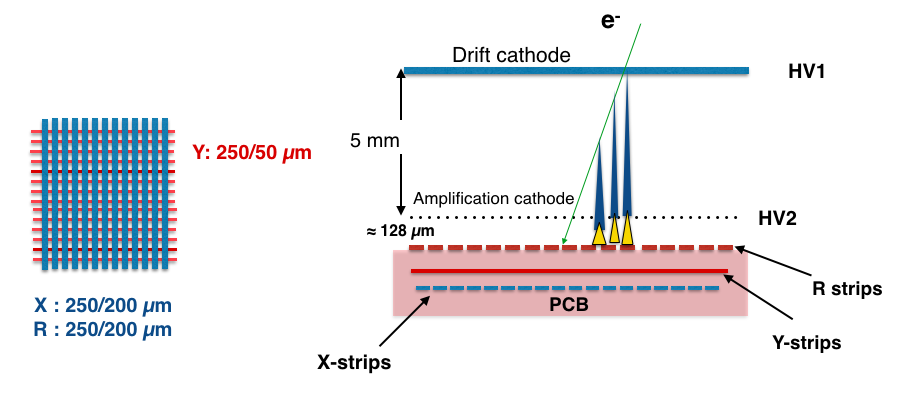
\includegraphics[width=\textwidth]{thesis_figures/NA64_MM.png}
\caption{Left: Strip dimensions of the modules, Right:NA64 Micromega's working principle~\cite{Banerjee:2017mdu}}
\label{fig:Micromegas_na64}
\end{figure}

\subsection{Gas Electron Multiplier}
\label{sec:GEM}

 \begin{figure}[t!]
 \centering
   \begin{minipage}[t]{.45\textwidth}
     \centering
     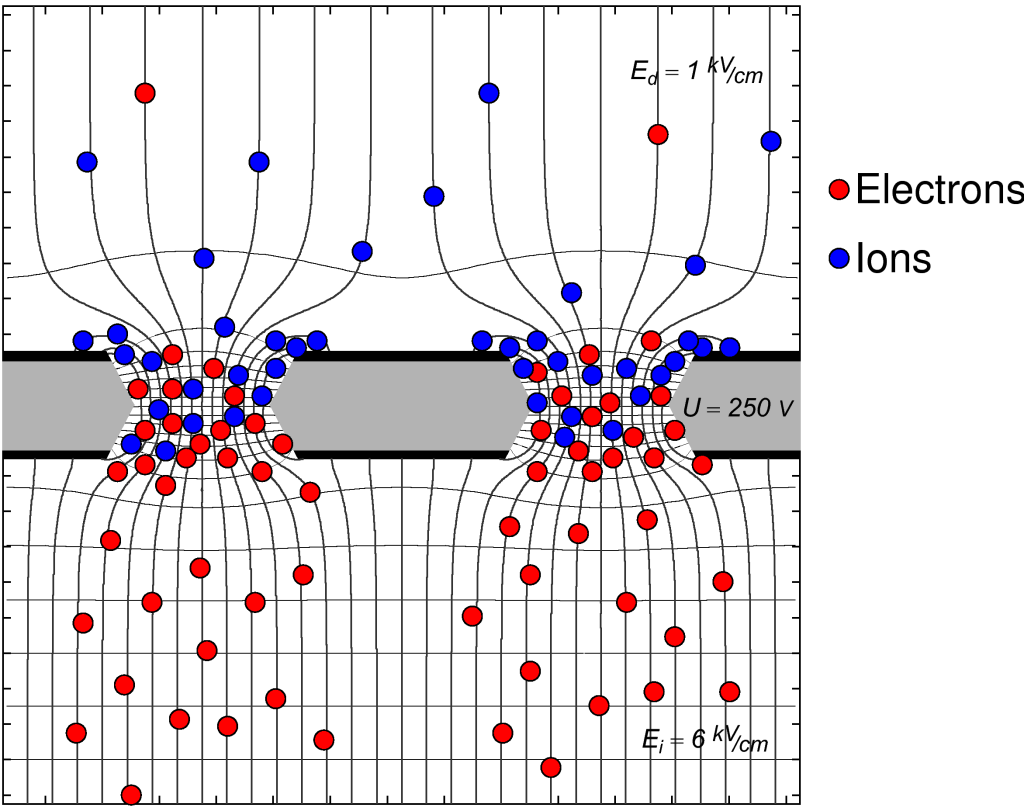
\includegraphics[width=\linewidth]{thesis_figures/GEM_field.png}

     \caption{A sketch of GEM field lines~\cite{GEM_field}.}
     \label{fig:GEM_field}
   \end{minipage}
   \hfill
   \begin{minipage}[t]{.45\textwidth}
     \centering
     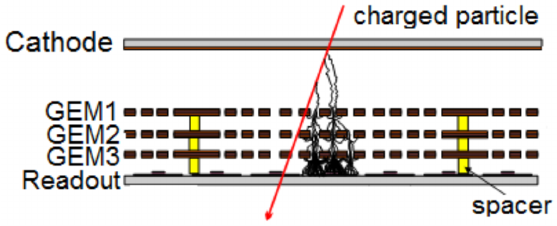
\includegraphics[width=\linewidth]{thesis_figures/GEM_process.png}
     \caption{Schematic of a triple GEM detector along with the working principle~\cite{article_GEM_pic}}
     \label{fig:Triple_GEM}
   \end{minipage}
 \end{figure}

\section{Track-Reconstruction Algorithm}

\subsection{Linear Regression}
\label{sec:Linear_Regression}
Linear regression for track fitting involves fitting a straight line to the data points, hits in our case with the condition that the total error is minimized. The total uncertainty is calculated as a sum of squares of individual measurement errors. Since the final result is dependent on minimizing the sum of the squares this approach to linear regression is known as least-squares approach. A simple mathematical description of the method is given below.

The equation of a straight line is given by $y=mx + c$, where $m$ is the slope of the line and $c$ is the intercept on the $y$ axis in a Cartesian coordinate system. The final goal is to obtain a good estimate for the two parameters $m$ and $c$. To obtain this estimate the square of error needs to be minimized. The error is the difference between the actual measurement $(x_i,y_i)$ and the prediction from our model, the equation of straight line. This error is also known as the residual and is defined as $r_i = y_i - m x_i - c $ for an $i^{th}$ measurement. Suppose that $n$ hits are measured then to obtain an estimate for $m$ and $c$ we need to minimize $\sum_{i=1}^n r_i^2$. The minimized estimates have the following values:
\begin{equation}
      \text{min}(m) = \frac{\sum_{i=1}^n x_i y-i - 1/n \sum_{i=1}^n x_i \sum_{i=1}^n y-i}{\sum_{i=1}^n x_i^2 - 1/n ()\sum_{i=1}^n x_i)^2}  = \frac{\bar{xy} - \bar{x}\bar{y}}{\bar{x^2-\bar{x}^2}}
\end{equation}
\begin{equation}
      \text{min}(c) = \bar{y} - \text{min}(m) \bar{x}
\end{equation}

A more detailed mathematical description can be found in \cite{Linear_regression}. The quality of the fit can be evaluated by calculating the reduced chi-square $\chi^2_{red}=\frac{\chi^2}{ndf.}=\frac{1}{ndf.}\sum_i \frac{(r_i)^2}{\sigma^2}$ where $\sigma$ is the resolution of each detector which might not be equal and ndf. are the number of degrees of freedom available for the fit.

Linear regression can also be used for NA64 to fit for the bending due to the magnets by replacing the model function from the equation of the straight line to some polynomial function. Such a method is called polynomial regression~\cite{STIGLER1974431}.

\begin{figure}[t!]
\centering
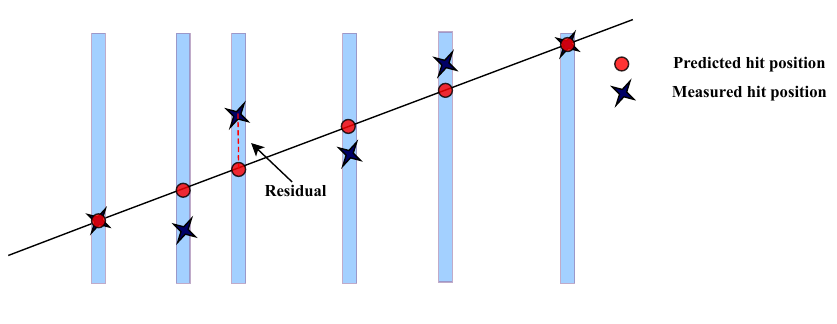
\includegraphics[width=\textwidth]{thesis_figures/linear_reg_new.png}
\caption{Linear regression pictorially. }
\label{fig:linear_regression}
\end{figure}

\begin{description}
  \item $\bullet$~\textbf{Filtering} is estimating the "present" state vector taking into account all the present and "past" measurements. Filtering from $m_1$ to $m_k$ includes filtering $m_1$ to $m_{k-1}$, then propagating from $m_{k-1}$ to $m_k$ and including $m_k$.
  \item $\bullet$~\textbf{Prediction} is estimating the state vector at a "future" time.
  \item $\bullet$~\textbf{Smoothing} is estimating the state vector at any point based on all the measurements.
\end{description}



%%% Local Variables:
%%% mode: latex
%%% TeX-master: "mythesis"
%%% End:

% !TEX root = mythesis.tex

%==============================================================================
\chapter{Detector exposure and Limits to the diffuse flux}
\label{sec:align}
%==============================================================================
 
The chapter aims to detail the procedure used to calculate the detector exposure or sensitivity to neutrinos for the DG$\mathrm{_{low}}$ region. The efficiencies calculated in the last chapter are used and the final expected neutrino rates are calculated. The first part of the chapter describes the exposure calculation along with the exposure contribution from different channels. Systematic uncertainties which can arise during the full analysis along with their contribution to the exposure are also discussed. 
The second part of the chapter details the results of the unblinding where no possible neutrino candidates were found for the angular range. Using this information an upper limit on the incoming flux of UHE $\nu$ is calculated. This limit is further compared to the one obtained by the previous analysis for the same time period but without the contribution of new triggers. The overall improvement forms a crucial result of this work. 


\section{Exposure Calculation}
\label{sec:det_exposure_calc}

One of the most accurate techniques used at Auger to calculate the exposure of the SD array to UHE$\nu$ is through extensive simulations of different detector configurations. In this method MC neutrino showers are thrown over varied detector configuration to calculate the effective or active area at each instant of time. Since the detector configuration of the SD array is constantly changing(\textit{faulty tanks, regular maintenance etc.}), sometimes on a daily basis, this technique requires a large amount of computational time and resources making it less desirable for use in this analysis. 

In this analysis, a different approach based on the 6T5 condition, which is required for each selected event in this analysis, is used for the exposure calculation. For this calculation, the 6T5 hexagon is taken to be the smallest possible detection unit for the $\nu$ event. The effective area i.e. the area seen by the incident cosmic neutrino for this detection unit at full efficiency is given by the Brillouin area~\cite{PierreAuger:2010zof}, $A_{6T5} = 1.95km^2$ as shown by the shaded area in fig~\ref{}. The aperture for this detector unit is dependent on the energy of the primary neutrino ,the slant depth in the atmosphere, X, neutrino flavor, type of the interaction, zenith angle, azimuth angel and the point of impact of the shower on the ground. The effective \textit{acceptance} of the detector unit can be written as follows:

\begin{equation}
  \label{eq:nu_accep}
  A_{hex}(E_{\nu}, X)  = \int^{\phi = 2\pi}_{\phi = 0} \,d\phi \int_{\theta_{min} = 58.5^{\circ}}^{\theta_{max}= 76.5^{\circ}}  \, A_{6T5} \cdot \varepsilon(E_{\nu}, X, \theta) \cdot sin\theta cos\theta \cdot d\theta    \mathrm{[cm^2 sr]}
\end{equation}

,where $\varepsilon(E_{\nu}, X, \theta)$ is the neutrino detection efficiency for each simulated energy, slant depth and zenith discussed in the last chapter. An example for a particular combination is given in fig.~\ref{}. Plots for efficiency for each combination can be found as part of the git code made available for this analysis. 

The next step involves integrating the \textit{acceptance} over the different simulated injected slant depths (as given in table~\ref{tab:Simulation_params}). This accounts for the \textit{effective mass} target for the neutrino identification over the 6T5 hexagon unit. It is calculated as follows. 

\begin{equation}
  \label{eq:nu_eff_mass}
  M_{hex}(E_{\nu}) = \int_X A_{hex}(E_{\nu}, X) \cdot dX
\end{equation}

Fig.~\ref{} shows the effective mass for both CC and NC interaction channels for a single 6T5 hexagon unit. Like the detection efficiency it increases with energy. 

Exposure calculation still needs to account for the detector configuration and its evolution over time. We reduced our array to units of 6T5 hexagons and a full SD array consisting of 1660 stations consists 1420 of these hexagons. Since the establishment of the Pierre Auger Observatory the active number of 6T5 hexagons are monitored every second. This forms a very good indicator for the time evolution of the SD array since any non-working station or large periods of instability are intrinsically recorded in the number of active 6T5 hexagons at that time. The instantaneous number of hexagons, $n_{hex}(t)$ thus can be used as an indicator of detector configurations over time. The $n_{hex}(t)$ were updated and calculated every minute and have an uncertainty of about 1.5\% as mentioned in~\cite{PierreAuger:2010zof}. To calculate the energy dependent exposure, the effective mass of one 6T5 hexagon is multiplied by the instantaneous number of hexagons and integrated in time. Further, the $\nu$ interaction probability for each flavour(i = $\nu_e, \nu_{\mu}, \nu_{\tau}$) and channel(c = CC, NC) is also folded in. The exposure is given as:

\begin{equation}
  \xi^{i,c}(E_{\nu}) = \frac{\sigma^{i,c}(E_{\nu})}{m_N} \int_{t} M_{hex}^{i,c}(E_{\nu}) \cdot n_{hex}(t) \cdot dt =  \frac{\sigma^{i,c}(E_{\nu})}{m_N} \cdot M_{hex}^{i,c}(E_{\nu}) \cdot N_{hex}
\end{equation}

,$\sigma^{i,c}(E_{\nu})$ is the neutrino nucleon cross-section~\cite{Cooper-Sarkar:2011jtt} and $N_{hex}$ is the total number of active 6T5 hexagons integrated in time over the search period. The value for $N_{hex}$ calculated for the period analysed is . The energy dependent exposure for different flavors and interaction channels is shown in fig~\ref{fig:Exp_flavors_comp}. It is necessary to point out again that the double bang showers which can be produced by $\nu_{tau}$ are not taken into account for this analysis which was also mentioned in sec.~\ref{sec:sim_DGL} 

\begin{figure}[t!]
  \centering
  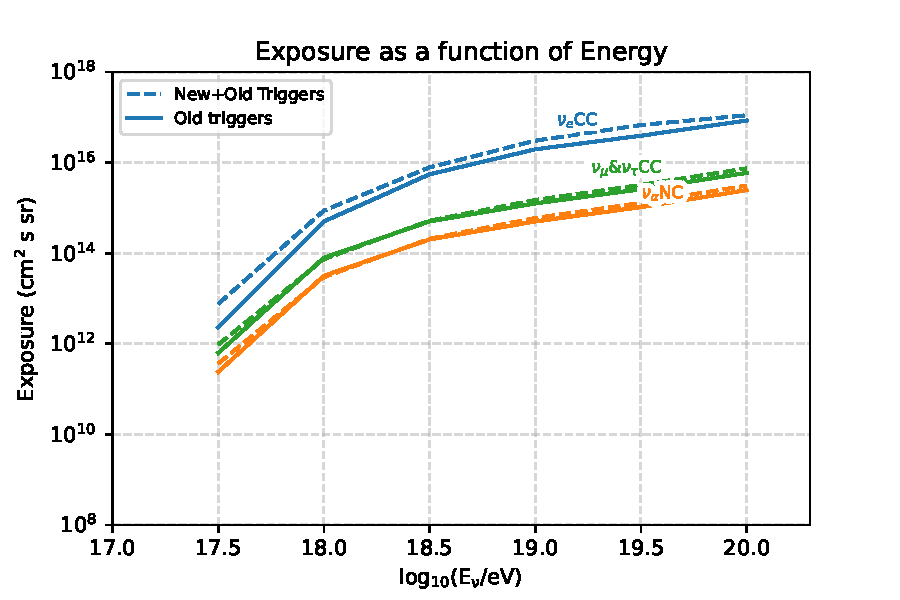
\includegraphics[width=14.5cm]{thesis_figures/ExpLimits/Exposure_comp_all_anotated_new_sim_optim.pdf}
  \caption{Exposure different channels}
  \label{fig:Exp_flavors_comp}
\end{figure}

An effective or total exposure, $\xi_{tot}(E_{\nu}) = \sum_{i}\sum_{c} \xi^{i,c}(E_{\nu})$ is calculated by summing all the interaction channels and assuming a 1:1:1 flavour ration at earth(large propagation distances combined with neutrino oscillations) as shown by the red line in fig~\ref{fig:Exp_total_comp}. 

\begin{figure}[t!]
  \centering
  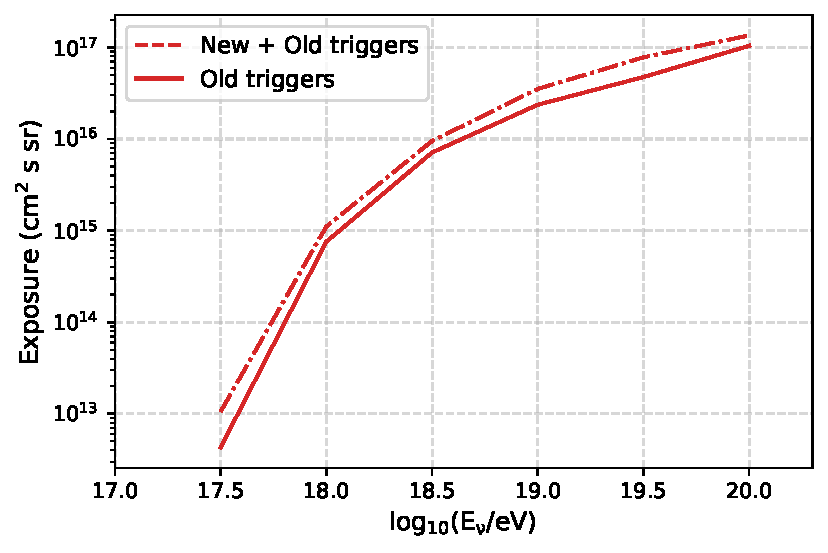
\includegraphics[width=14.5cm]{thesis_figures/ExpLimits/Exposure_comp_total_new_sim_optim.pdf}
  \caption{Total exposure}
  \label{fig:Exp_total_comp}
\end{figure}

As seen in the figure the $\nu_e$ CC channels contributes the most to the total neutrino exposure($\sim$85\%). The exposure rises rapidly at lower energies and then mostly flattens with just a slight increase which is due to the energy dependent neutrino cross-section. The shape is due to the neutrino detection efficiency which is small at lower energies as shown in fig~\ref{} in the last chapter. The next dominant channels are the $\nu_{\tau}$ and $\nu_{\mu}$ which have a similar detection efficiency as the NC channel but have a higher value of cross-section. The NC channel contribution is very small($\sim$5\%) due to the reasons discussed in section ~\ref{subsec:nu_sel_nudeteff}.  

The exposure calculated this analysis is compared to the one calculated using the previous analysis for the same time period in fig~\ref{fig:Exp_flavors_comp}. For the CC channel a 5x improvement is seen at lower energies and a 2x improvement at higher energies. For NC this improvement is not that significant. There is a 2x improvement at lower energies and a 1.5x improvement at higher energies. The improvement at lower energies is due to the inclusion of the new triggers MoPS and ToTd which enhance the detection efficiency at lower energies. The improvement at higher energies is mainly due to the improved Fisher analysis. The total exposure is also improved by a factor of ... 

\section{Systematic uncertainties}
\label{sec:det_uncert}
\todo{Determine what to write}
HERWIG PYTHIA difference take from old analysis.
PDF difference what is this ?
Hadronic interaction calculate yourself for 72 deg and $10^{19}$eV
https://scipost.org/SciPostPhysProc.13.028/pdf for CORSIKA vs others.
GAP2010-027 sytematic uncertainities neutrinos 
Also consider tau energy Loss maybe already mentioned in 2010 neutrino paper. 
Offline fluctuations and different reconstruction algorithms quote your own work.
can also quote An improved limit to the diffuse flux of ultra-high energy neutrinos
from the Pierre Auger Observatory(doi:10.1103/PhysRevD.91.092008) 
\section{Data unblinding}
\label{sec:data_unblinding}
As mentioned before in section~\ref{subsec:nu_sel_samp} the search data comprises of all events recorded at the Observatory between 2014-2021 which have a SD ID number non-divisible by 5 i.e. 80\% of all SD data recorded between 2014-2021. This search data sample was further split into a 20\% test sample similarly where SD ID numbers divisible by 4 were taken to be a part of the test sample while the rest became the part of the 60\% search sample. This split was done to perform the unblinding in two stages. The first where only the test sample in unblinded to detect any flaws with the analysis and if and when those flaws are fixed, the rest of the data is unblinded. This exercise turned out to be useful as a slight flaw was uncovered during the unblinding process of the 20\% test sample which was corrected. Said flaw which is described in more detail later required the whole reconstruction process along with the training of the Fisher polynomial to be performed again. This also led to the unblinded 20\% test sample to be blinded again since the reconstruction was altered. The splitting procedure was repeated and the total unblinding was performed again in parts. It is important to mention in all of unblinding procedure \textbf{0 neutrino events survive} the analysis selection.
This section is thus split into two subsections. The first describing the unblinding of the 20\% test sample along with the changes brought about by this unblinding. The second section details the full unblinding of the redone search samples (test + remaining) and discusses the interesting features of the unblinded search samples. 

\subsection{20\% test sample}
\label{subsec:unblind_20}

\todo{Test sample before the reco changes:}
% \begin{figure}[t!]
%   \centering
%   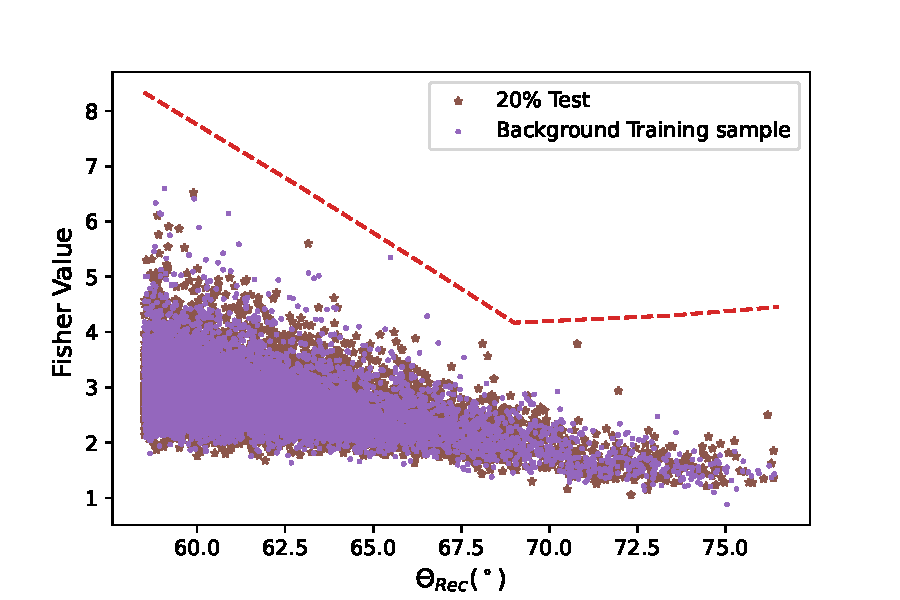
\includegraphics[width=14.5cm]{thesis_figures/Nu_analysis/Fisher_plots/Fisher_comp_bkg_test_wnt.pdf}
%   \caption{Test_reval vs background}
%   \label{fig:Fish_bkg_test}
% \end{figure}

The Fisher value distribution for the test sample is shown in fig~\ref{}. As it is shown no event passes the Fisher cut in any angular region. However, there are a few events which come very close to the cut line. Five events marked with a red circle were analysed in more detail. Each of them has its own unique reason with only the one with zenith~ being the most interesting. This event has the ID of 66106356. After looking at detailed information about the event it was found out that the accidental station cut used is insufficient. Previously, the  accidental cut (rejection of stations with Totalsignal < 3 VEM) is only applied to the event if there are more than 5 stations in the event. Since for this analysis due to the inclusion of MoPS and ToTd an overall increase in events is expected which also increases the overall number of stations with accidental stations this cut needs to be reduced a bit to take this overall increase into account. Thus, this cut was reduced to apply for events with more than 4 stations. This reduction of the cut decreases the total events passing the analysis cut by $\sim$5\% for the background training sample and $1-2$\% for the signal training sample. The Fisher coefficients and cut changes slightly. After this change in the reconstruction the test sample was obtained again and compared to the background dample as shown in fig~\ref{fig:Fish_bkg_test}. The other interesting events which have $\mathcal{F}$ values close to the $\mathcal{F_{cut}}$ with their respective ids are tabulated in table~\ref{}. These events were individually evaluated. Some of these () were found to have a bad time residual fit primarily because of multiple peaks observed in stations triggered by the new triggers. Since, no segmentation algorithm was used for stations with MoPS and ToTd triggers sometimes a wrong peak was selected which affected the reconstruction for these events. A future analysis with a corrected segmentation algorithm which is functional for the new triggers MoPS and ToTd is envisaged in the future analysis upgrades. Such events are expected to be limited to less than $\sim$1\% of total events but still require a careful look for future analysis upgrades. A further detailed analysis was also performed for these events where the primary mass composition was extracted via the muon production distributions as mentioned in~\cite{PierreAuger:2014zay}. Even with large uncertainties these events are most likely due to a light deep primary. For the other three events no particular feature worth mentioning was observed. 

\begin{figure}[t!]
  \centering
  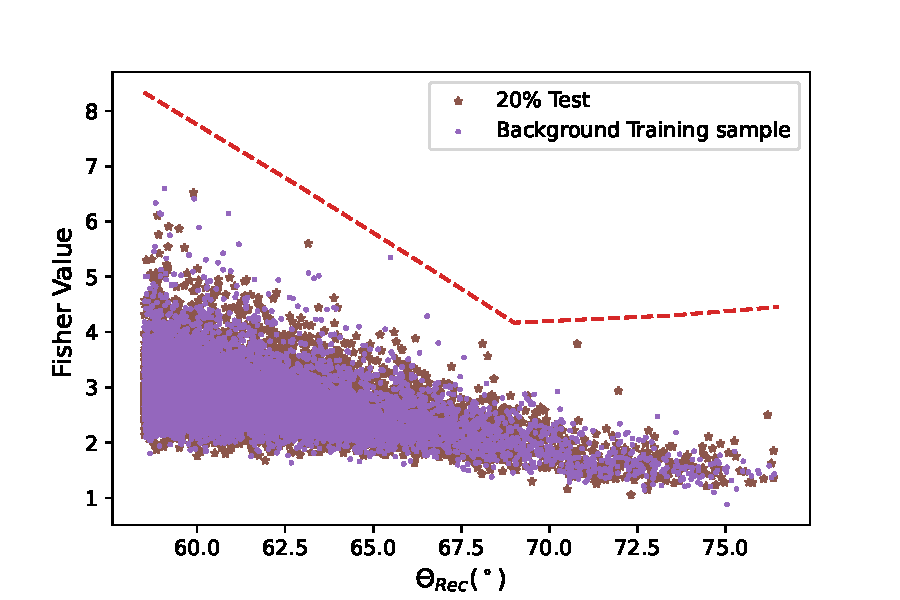
\includegraphics[width=14.5cm]{thesis_figures/Nu_analysis/Fisher_plots/Fisher_comp_bkg_test_wnt.pdf}
  \caption{Test_reval vs background}
  \label{fig:Fish_bkg_test}
\end{figure}

\begin{figure}[t!]
  \centering
  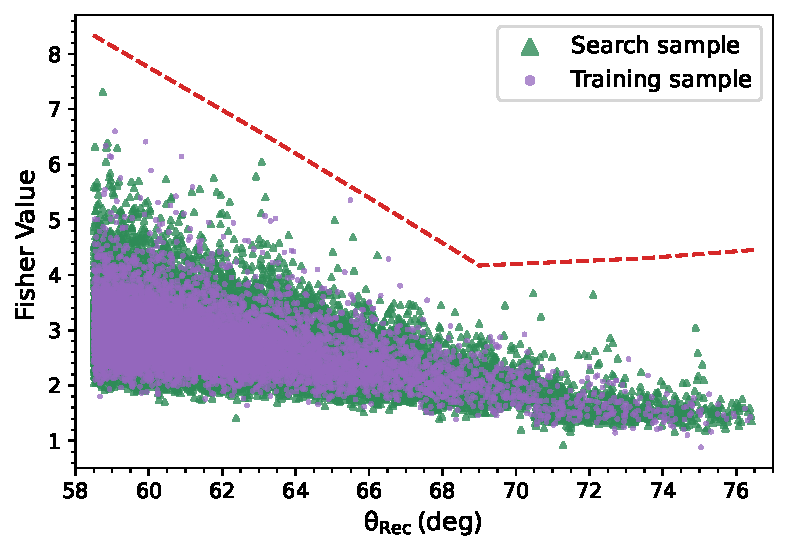
\includegraphics[width=14.5cm]{thesis_figures/Nu_analysis/Fisher_plots/Fisher_comp_bkg_search_wnt.pdf}
  \caption{Search vs background}
  \label{fig:Fish_bkg_test}
\end{figure}

\subsection{Reevaluated 20\% test search sample and 60\% search sample}
\label{subsec:unblind_60}
After the unblinding of the test sample and changing the cut mentioned in the section above, the unblinding was again performed in two stages. Initially a 20\% part was unblinded and then the remaining 60\% blinded sample was analysed. Again \textbf{0 neutrino candidates} were found after candidate selection. The results of the unblinding for each sub-angular bin is presented in fig~\ref{fig:Fisher_cut_2} along with the Fisher value as a function of zenith angle presented in fig~\ref{}. The results (red) are overlaid over the training(orange) and test (blue) samples with the dashed lines indicating the value of the $\mathcal{F_{cut}}$ obtained according to eq.~\ref{eq:fisher_poly_cut}. As it can be seen the distributions are compatible to each other within statistical fluctuations. The overlay also confirms that the exponential tail assumption is a reasonable enough to determine the $mathcal{F_{cut}}$. The goodness of the fit is once against presented in tab.~\ref{tab:Cut_eval_unblind} in the form similar to table~\ref{tab:Cut_eval}. This time for the observed values the numbers are calculated from the much larger search sample. It is found that the tails of the distributions which typically seemed to have fit badly also fit reasonably well. The events in the search sample that have $\mathcal{F}$ values close to the $\mathcal{F_{cut}}$ were again carefully checked and were found to be either due to the issues with the segmentation algorithm or known issues such as partial shower containment or large number of non-working PMTs both issues have also been seen in previous analysis. 

\begin{figure}[h!]
  \centering
   \begin{subfigure}[l]{.48\textwidth}
     \centering
     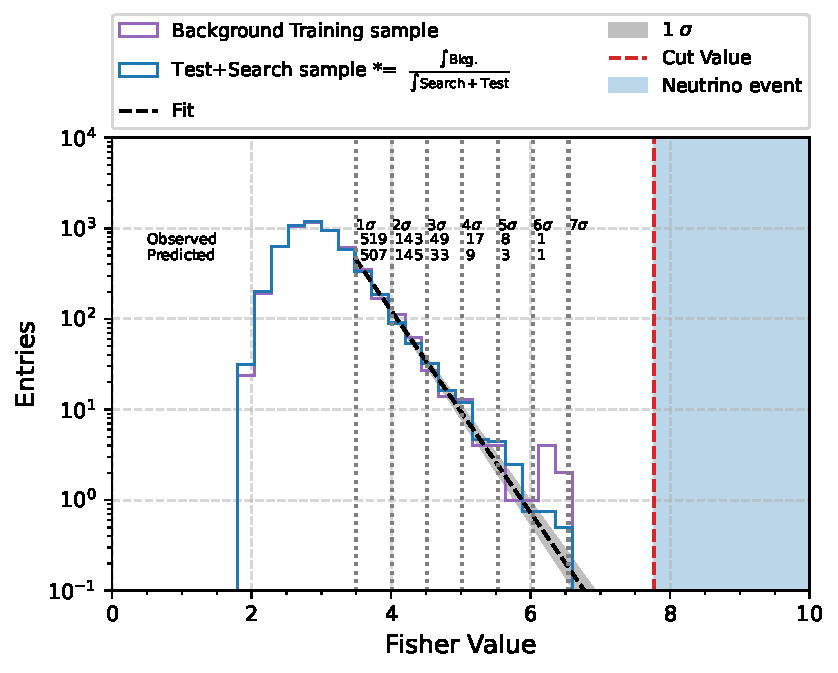
\includegraphics[width=\linewidth]{thesis_figures/Nu_analysis/Fisher_plots/Fisher_fit_search+test_bkg_region_58.5_61.5.pdf}
     \caption{58.5 61.5}
     \label{fig:58.5-61.5}
   \end{subfigure}
   %\hfill
   \begin{subfigure}[r]{.48\textwidth}
     \centering
     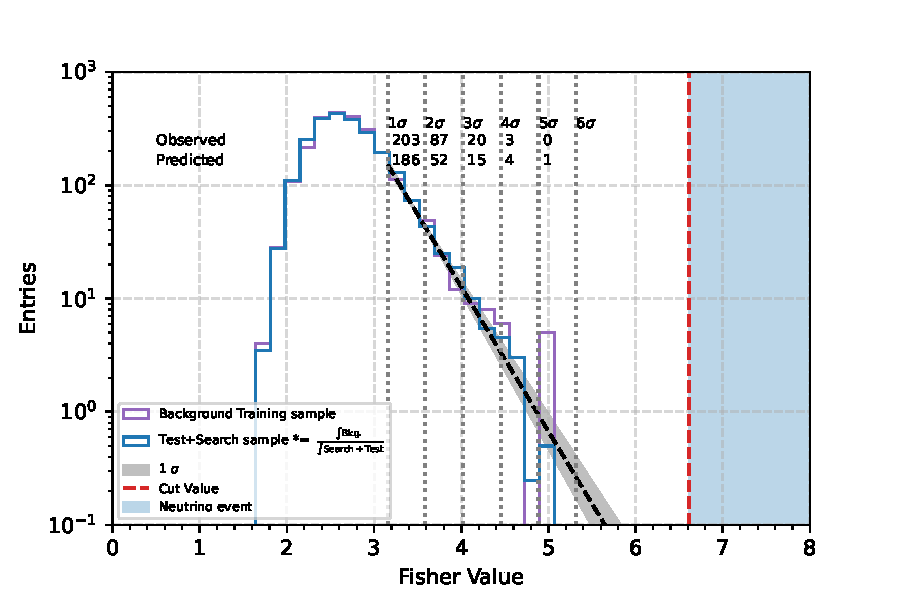
\includegraphics[width=\linewidth]{thesis_figures/Nu_analysis/Fisher_plots/Fisher_fit_search+test_bkg_region_61.5_64.5.pdf}
     \caption{61.5 64.5}
    \end{subfigure}
    \hfill
    \begin{subfigure}[l]{.48\textwidth}
      \centering
      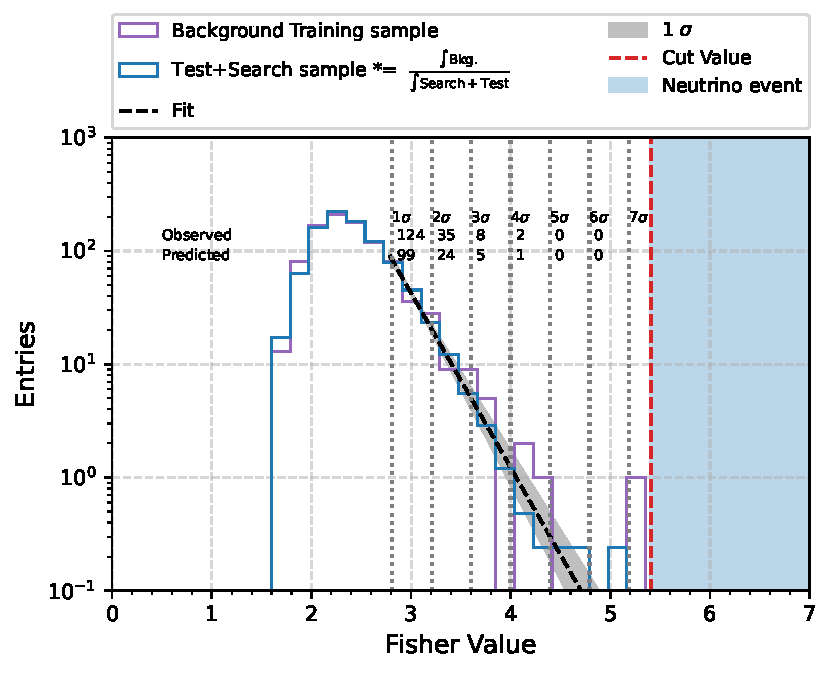
\includegraphics[width=\linewidth]{thesis_figures/Nu_analysis/Fisher_plots/Fisher_fit_search+test_bkg_region_64.5_67.5.pdf}
      \caption{64.5 67.5}
    \end{subfigure}

    \begin{subfigure}[r]{.48\textwidth}
      \centering
      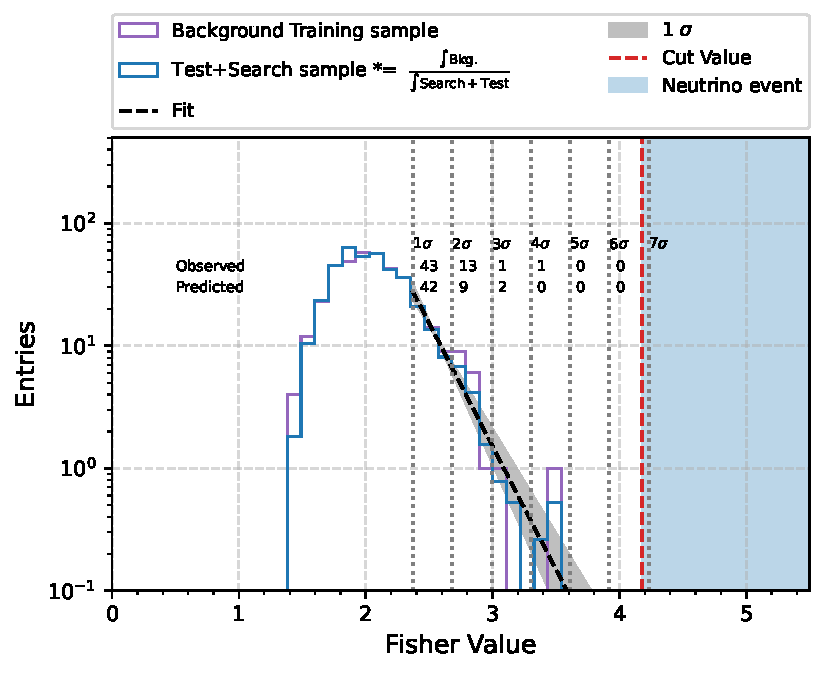
\includegraphics[width=\linewidth]{thesis_figures/Nu_analysis/Fisher_plots/Fisher_fit_search+test_bkg_region_67.5_70.5.pdf}
      \caption{67.5 70.5}
    \end{subfigure}
    \hfill    
    \begin{subfigure}[r]{.48\textwidth}
      \centering
      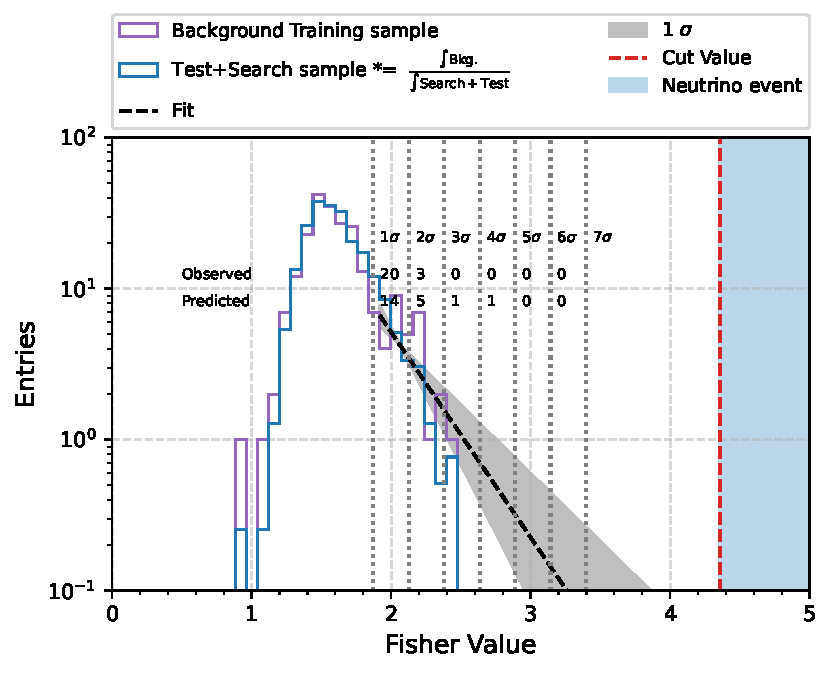
\includegraphics[width=\linewidth]{thesis_figures/Nu_analysis/Fisher_plots/Fisher_fit_search+test_bkg_region_70.5_73.5.pdf}
      \caption{70.5 76.5}
   \end{subfigure}
   \caption{Evaluating the goodness of fit of the Fisher cut for the search sample. The observed values are compared to the predicted values.}
    \label{fig:Fisher_cut_2}

\end{figure}

\begin{table}[h!]
  \centering
  \begin{tabular}{ |P{1.25cm}||P{2.4cm}|P{2.4cm}|P{2.4cm}|P{2.4cm}|P{2.4cm}| }
    \hline
      Fit & \multicolumn{5}{c|}{Number of events in $\mathcal{F}$ tails} \\
      Range & \multicolumn{5}{c|}{Observed - Predicted} \\
    \cline{2-6}
      & Region 1 & Region 2& Region 3& Region 4 & Region 5 \\
      &(58.5$^\circ$-61.5$^\circ$]&(61.5$^\circ$-64.5$^\circ$]&(64.5$^\circ$-67.5$^\circ$]& (67.5$^\circ$-70.5$^\circ$] & (70.5$^\circ$- 76.5$^\circ$] \\
    \hline 
    $\mu$ + 1$\sigma$ & 13 & 14 & 17 & 19 & 23 \\
    $\mu$ + 2$\sigma$ & 1640 & 1820 & 2040 & 2330 & 2720 \\
    $\mu$ + 3$\sigma$ & 140 & 220 & 140 & 230 & 120 \\
    $\mu$ + 4$\sigma$ & 140 & 220 & 140 & 230 & 120 \\
    $\mu$ + 5$\sigma$ & 140 & 220 & 140 & 230 & 120 \\
    $\mu$ + 6$\sigma$ & 140 & 220 & 140 & 230 & 120 \\
    \hline
  \end{tabular}
  \caption{Table to test captions and labels.}
  \label{tab:Cut_eval_unblind}
\end{table}
\section{Diffuse limit for the UHE neutrino flux}
\label{sec:diff_limit}
Since no neutrino candidate was found in this analysis, an upper limit to the flux of the incoming UHE$\nu_s$ can be evaluated. Let flux per unit area, \textit{A}, energy, solid angle $\omega$ and time be denoted by $\mathrm{\phi(E_{\nu}) = \frac{d^6 N_{\nu}}{dE_{\nu}d\omega dA dt}}$. The expected number of detected neutrinos can be calculated by folding in the total exposure $\xi_{tot}(E_{\nu})$ with flux as follows,

\begin{equation}
  \mathrm{N_{expected} = \int_{E_{\nu min}}^{E_{\nu max}} \phi(E_{\nu}) \cdot \xi_{tot}(E_{\nu}) \cdot dE_{\nu}}
\end{equation}

Assuming a differential UHE$\nu$ flux $\phi = k \cdot E_{\nu}^{-2}$, the integrated upper limit on the value of k is given by:

\begin{equation}
  \label{eq:integ_lim}
  \mathrm{k_{up} = \frac{N_{up}}{\int_{E_{\nu min}}^{E_{\nu max}} E_{\nu}^{-2} \cdot \xi_{tot}(E_{\nu}) \cdot dE_{\nu}}}
\end{equation}

, the value of $\mathrm{N_{up}}$ for a given confidence level can be determined based on the number of observed events and the number of expected background events. Different statistical methods can be used to obtain the value for $N_{up}$ based on the confidence interval. In the next sections some of these different statistical approaches are discussed in more detail. The Feldman and Cousins limit with an extension that incorporates the systematic uncertainties discussed above is chosen as a final estimate for $\mathrm{N_{up}}$.

\subsection{Feldman and Cousins limit}
\label{subsec:FandC}
Feldman-Cousins method~\cite{Feldman:1997qc} is a statistical technique used to construct confidence intervals, particularly for Poisson distributed data. This approach addressed the key shortcomings of traditional methods used to construct confidence intervals especially for cases where the number of observed events are low or zero. Traditional methods such as Gaussian approximation, which assumes that data follows a normal distribution which are used to calculate confidence intervals can often lead to incorrect interval particularly in rare event searches where the data is better described by a Poisson distribution. This can also lead to unphysical values e.g. negative value for rate of expected events. The Feldman-Cousins approach solves these problems by giving a unified method for constructing confidence intervals. The method ensures that the intervals are unbiased and do not favour one outcome over the other. It also ensures natural transition from two-sided intervals(where there is significant data) to one-sided upper limits(when there is little to no data). The method also respects physical constraints, such as non-negative value for expected event rates. It also provides intervals with more accurate coverage probabilities, reducing over-coverage issues common in other methods. 

The Feldman \& Cousins approach is implemented as a part of \textit{gammapy} in python~\cite{Gammapy:2023gvb} which was used  to get the interval for this analysis. The information was also verified with look-up tables in~\cite{Feldman:1997qc}. For a 90\% confidence interval, in case of zero signal and background events, the upper and lower limits are given as $N^{90\%}_{up} = 2.44$ and $N^{90\%}_{low} = 0$ respectively. If one signal event is seen with zero background then this interval shifts to [4.36,0.11]. It is important to note that both statistical and systematic uncertainties are not included for the intervals calculated in the Feldman \& Cousins method. 

\subsection{Rolke approach}
\label{subsec:Rolke}
The Feldman \& Cousins treatment is a frequentist method which requires the background source to be known precisely. Such a method can fail if the uncertainties are too high~\cite{Rolke:2000ij}. To solve this problem one can also use the Rolke method~\cite{Rolke:2004mj} which incorporates prior information in this case signal with a Poisson distribution and background with either a Poisson or Gaussian distribution. The method is implemented as a ROOT class under TRolke~\cite{TRolke_ROOT}. For a 90\% confidence interval in the case of zero signal and background events the interval is given as [2.21,0] assuming a Poisson distribution for both signal and background. As it is seen the interval is smaller in comparison to the Feldman \& Cousins approach. This can be explained much more clearly for the case where there is one signal event and no background where the Rolke interval is [3.65,0]. In this case according to the Feldman \& Cousins approach the event has to be a signal since the lower limit is > 0 but in the Rolke approach it is still possible that such an event in the signal region could be a background event i.e. in the Rolke approach the absence of background does not imply zero background, but it only means that the background is not too large. This is because background is treated as a Poisson number. Thus, the overall upper and lower limits in the Rolke approach are always smaller in comparison to the Feldman \& Cousins  method. 

\subsection{Conrad approach}
\label{subsec:Conrad}
The Conrad method for calculating confidence intervals allows the inclusion of systematic uncertainties in the evaluation. Using this approach the uncertainties in the background prediction, background detection and the signal detection efficiencies can be incorporated in the confidence interval calculation by integrating over the PDFs of these parameters~\cite{Conrad:2002kn}. The method computes the upper limit based on a likelihood ratio between the observed data and the null hypothesis(no signal). For this work the interval was calculated using POLE++~\cite{Conrad:2005zm} which is a C++ program that implements the Conrad method. The systematic uncertainty on exposure was estimated to be as [] as mentioned in section~\ref{sec:det_uncert}. Using a uniform PDF to characterise the exposure and a Gaussian assumption for background, for a 90\% confidence interval in the case of zero signal and background events the upper and lower limits are given as: 

\begin{equation}
  \label{eq:Conrad_lim}
  N^{90\%}_{up} = 2.39\\
  \, N^{90\%}_{low} = 0
\end{equation}

The interval is smaller in comparison to the Feldman \& Cousins method due to the uneven interval for the systematic uncertainty. For one signal event and zero background the interval changes to []. 

\subsection{Final calculation}
\label{subsec:final_lim}
After the determination of $N_{up}$ using the Conrad approach the equation~\ref{eq:integ_lim} can be solved to determine the upper limit to the diffused flux of UHE$\nu_s$. The integral goes from $E_min = 10^{17.5} $eV till $E_max = 10^{20.5} $eV which is the total energy range explored in the simulations. It is also important to note that the limit is only valid for a smaller energy window. The single flavour 90\% C.L. integrated limit is given by 
\begin{equation}
  \label{eq:final_lim}
  \mathrm{k_{90} < 6.3 x 10^{-17} GeV cm^{-2} s^{-1} sr^{-1}},
\end{equation}
It applies to an energy range of $E_{\nu} \epsilon [1.9 \times 10^{18} - 2.0 \times 10^{20}]$ which is the energy range for which $\sim$90\% total event rate is expected in the case of $E^{-2}_{nu}$ flux. The value along with the 90\% energy range is plotted as a solid line in fig~\ref{}.

\begin{figure}[t!]
  \centering
  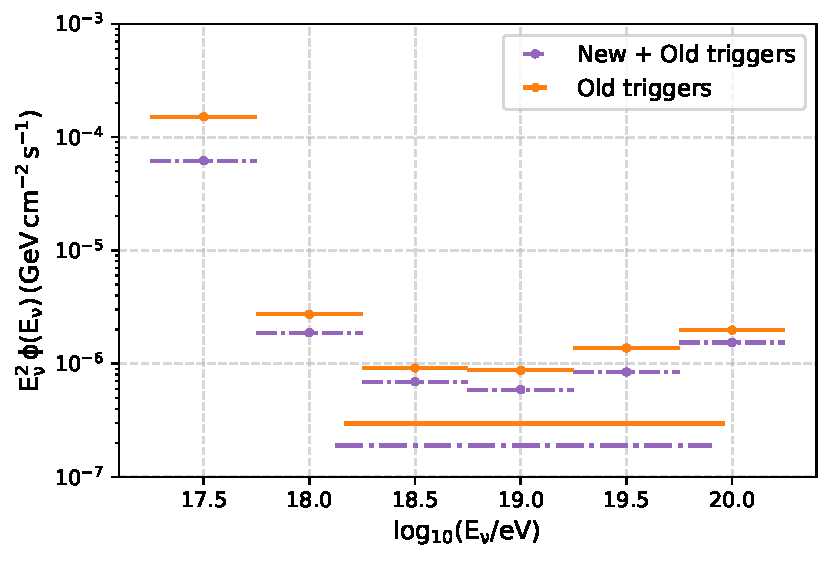
\includegraphics[width=14.5cm]{thesis_figures/ExpLimits/Integ_DiffLimit_comp_new_sim_optim.pdf}
  \caption{Diff limit new old comparison}
  \label{fig:Limit_comp_1}
\end{figure}

The other lines in green are the \textit{differential limits}. These are calculated by integrating the denominator of eq.~\ref{eq:integ_lim} in bins of width $\Delta = 0.5eV$ in $log_{10}(E_{\nu})$. Mathematically for the $i^{th}$ bin this can be represented as follows:

\begin{equation}
  \label{eq:diff_lim}
  \mathrm{Differential \,limit \, (i^{th} \, E_{\nu} \, bin)  = \frac{N_{Up}}{\int_{log_10(E^i - (\Delta log_{10}E)/2)}^{log_10(E^i + (\Delta log_{10}E)/2)} E^{-1}_{\nu} \cdot \xi(E_{\nu}) \cdot ln(10) \cdot d(log_{10}(E_{\nu}))}}
\end{equation}

Assuming constant exposure and flux in each energy bin the differential limit can be estimated as:

\begin{equation}
  \label{eq:diff_lim_approx}
  \mathrm{Approx. \, Differential \,limit \, (i^{th} \, E_{\nu} \, bin)  = \frac{N_{Up}}{E^{-1}_{\nu} \cdot \xi(E_{\nu}) \cdot ln(10) \cdot \Delta (log_{10}(E_{\nu}))}}
\end{equation}

These limits provide a way to denote the sensitivity of the detector for different energies. As it can be seen from the fig.~\ref{fig:Limit_comp_1} for the Down-going Low analysis the Pierre Auger Observatory is the most sensitive for energies $\sim$1 EeV. 

Both limits are also compared to the results from the previous analysis in fig~\ref{fig:Limit_comp_1}. As it was seen in the exposure comparison it is clear that the new triggers help improve the sensitivity at lower energies. For higher energies the improvements to the upper-limit for the diffuse flux of $UHE_{\nu_s}$ though not as signifivcant is still substantial. This improvement can be attributed to the changes in the Fisher analysis The integral flux limit sees an improvement $\sim$.. order of magnitude. The aim of this study was to evaluate the improvement, but it was always know that for this angular range significant improvements to the diffuse flux improvements were not expected. The diffuse flux limit and sensitivity for Auger is dominated by the Earth-skimming channel as shown in ~\cite{Aab_2019_diffuse}. This limit is significantly lower than the DG$\mathrm{_{low}}$ channel and is the main driver to constrain astrophysical and cosmogenic models. However, the improvements shown in this analysis are more important in the context of point source searches. This is discussed more in the next chapter. 

\begin{figure}[t!]
  \centering
  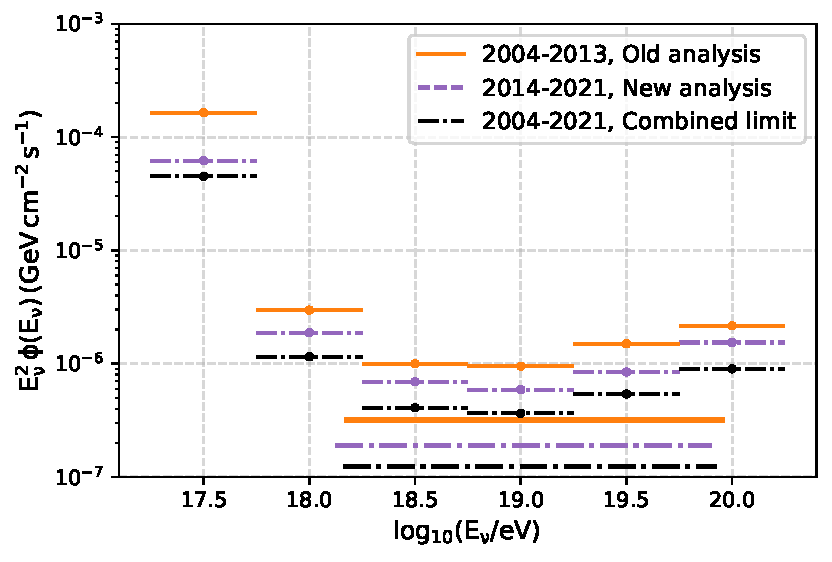
\includegraphics[width=14.5cm]{thesis_figures/ExpLimits/Integ_DiffLimit_comp_combined_new_sim_optim.pdf}
  \caption{Diff limit combination}
  \label{fig:Limit_comp_2}
\end{figure}

\begin{figure}[t!]
  \centering
  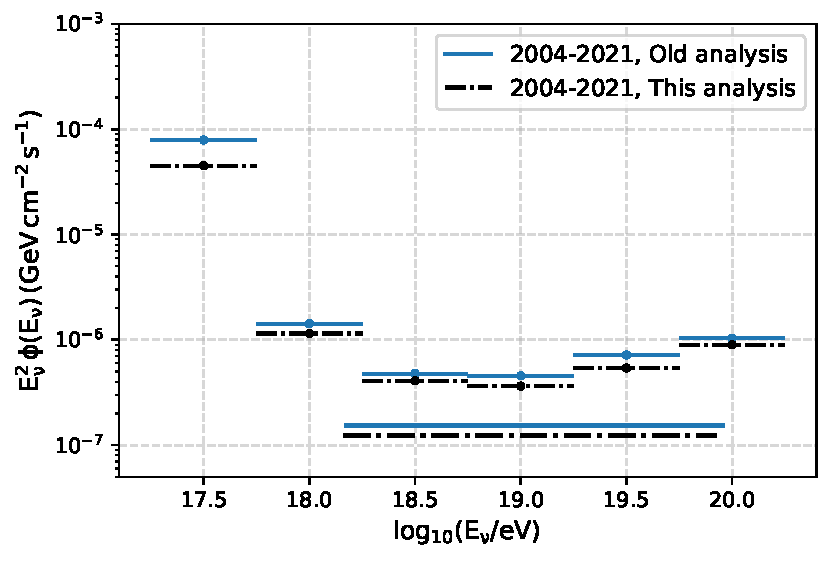
\includegraphics[width=14.5cm]{thesis_figures/ExpLimits/Integ_DiffLimit_comp_combined_new_sim_optim_3.pdf}
  \caption{Diff limit combination}
  \label{fig:Limit_comp_3}
\end{figure}


%%% Local Variables:
%%% mode: latex
%%% TeX-master: "mythesis"
%%% End:

% !TEX root = mythesis.tex

%==============================================================================
\chapter{Source follow-up analysis}
\label{chap:follow-up}
%==============================================================================

One of the most exciting fields of modern day neutrino astrophysics involves scanning the observable sky to look for neutrino sources. As mentioned in section~\ref{} the observation of TXS~\cite{} and NGC 1068~\cite{} which are examples of a transient source and a steady state of neutrinos has brought unprecedented excitement to the field. Any observation of a neutrino source offers a chance to significantly increase our overall knowledge about astroparticle physics. Since, Auger is one of the few experiments in the world sensitive to UHE$\nu_s$ any improvement in its point source sensitivity increases its capability for neutrino detection. 

In this chapter the point source sensitivity to $\nu$ events of the SD array is discussed for the zenith angular range explored in this thesis, DG$_{low}$. Based on the zero neutrino candidates found in the search performed in this work a source declination, $\delta$ dependent neutrino flux is calculated. This process includes calculating the declination dependent exposure and then converting it to a limit on the flux. The improvements to this exposure and sensitivity by the inclusion of new triggers is also discussed. Finally, the new limit is used to scan a few interesting sources which lie in the most sensitive range for the DG$_{low}$ region.

\section{Procedure for point source analysis}
\label{sec:procedure_point_source}

\subsection{Source visibility}
\label{subsec:psource_coverage}
The field of view of the Observatory and the corresponding neutrino efficiency is related to the zenith angle which in turn is related to declination. For a given point like source at declination $\delta$ and right ascension $\alpha$(in equatorial coordinates), the time zenith angle, $\theta$ dependence at a certain time, $t$ is given by:
\begin{equation}
  cos \theta(t) = sin \lambda \,sin \delta+ cos \lambda \, cos \delta \,sin (2\pi \frac{t}{T} - \alpha)
\end{equation} 
where $T$ is the duration of one sidereal day and $\lambda$ is the latitude of the observer($\lambda = -35.2^{\circ}$ for Auger). 
Fig.~\ref{} shows the FOV bands for different neutrino search channels(DGL, DGH, ES). These bands are plotted in equitorial coordinates as a function of $\alpha - t _{GS}$ where $t_{GS}$ is the Greenwich Sidereal Time(GST) converted to for a mean longitude of the Observatory, $l$ calculated as $t_{GS}= 2\pi t/T + l$. The sensitive declination ranges for different $t_{GS}$ can be read from the plot which is very useful for real-time transient follow-up. For DGL showers the SD of the Pierre AUger Observatory is sensitive to declinations between $\delta ~ -85^{\circ} - 40^{\circ}$. Another way to denote sky coverage for different neutrino searches at Auger is by calculating the time a source is visible to the Observatory for a particular declination. This is plotted in fig.~\ref{} for all three search channels. As it can be seen from the plot all three channels are the most sensitive at two ends of their sensitive declination ranges(DGL $\delta ~ -70^{\circ}, 35^{\circ}$) which is a consequence of smaller variation in zenith angle in time for certain directions. The sensitivity sharply decreases beyond these declination values. In the middle of these \textit{two horns} is a plateau like region. It is also seen that generally the fraction of time a source is visible is comparable in the DG$_{low}$ and DG$_{high}$ range with both being higher in the ES range due to the size of the zenith angle windows. The fraction of visible time for vertical showers is also plotted. Even though this fraction of time is significantly high no neutrino search can be performed for this region as it is very difficult to differentiate between a cosmic ray and neutrino shower for this zenith angle range. 

\subsection{Effective area and Exposure}
\label{subsec:psource_area}
Following this to calculate point source sensitivity, the declination dependent SD exposure is evaluated. This is done by first calculating an effective area to neutrinos of flavours i and energy $E_{\nu}$ is defined in the following way. For a point source spectral flux of flavour $i$ given by $\phi_i(E_{\nu}) = \frac{d^4 N_{\nu}}{dE_{\nu} dA dt}$ the expected number of detected events is given by 

\begin{equation}
  \frac{dN_{i}}{dt} = \int_{E_{\nu min}}^{E_{\nu max}} \, dE_{\nu} \, \phi(E_{\nu}) \, \mathcal{A}_i(E_{\nu})
\end{equation}
The effective area is flavour dependent since for each flavour the shower development and the primary interaction(c = NC, CC) is substantially different. The effective area is for the DGL region is given as follows:
\begin{equation}
  \mathcal{A_{i,c}}(E_{\nu},\theta(t),t) = \frac{\sigma^{i,c}(E_{\nu})}{m_N} \int_{X} \, \varepsilon_{i,c}(E_{\nu},\theta(t),t) A_{6T5} n_{hex}(t) dX
\end{equation}

where $\varepsilon_{i,c}$ is the neutrino identification efficiency for a 6T5 unit. The declination dependence is taken into account by the $\theta(t)$ dependence of the efficiency. The effective area for electron neutrinos with CC interactions in km$^2$ for 2016 array and different theta is plotted in fig.~\ref{}. The effective area increases with increasing primary energy. It also increases with zenith angles till ~70$^\circ$ after which there is a slight decrease in the effective area which is due to the decrease in neutrino sensitivity at higher zenith angles discussed earlier in section~\ref{}. 

The exposure to point-like sources of UHE neutrinos can then be calculated by integrating the effective area for a given time interval and summing over the different flavours and channels as follows:
\begin{equation}
  \xi(E_{nu}, \delta) = \sum_{i,c} \int_{t} \mathcal{A_{i,c}}(E_{\nu},\theta(t),t) dt
\end{equation}

The exposure is $\delta$ dependent due to the dependence of effective area on $\theta(t)$. The effective area can also change with time due to the changes in the number of hexagons $n_{hex}(t)$. This change has been visualized for the DG$_{low}$ channel for the time period of this search in fig.~\ref{}. As it can be seen in the plot the number is relatively stable especially in the period of one sidereal day apart from few outages which are removed from the searches. The directional exposure for the DGL channels for different fixed energies between 2014-2021 is shown in fig.~\ref{}. The solid line shows the exposure calculated in this study by including the new triggers while the dashed line shows the exposure calculated with the previous analysis for the same time period. Similar to the exposure calculated for the diffuse flux the exposure is significantly improved for lower energies with the improvement decreasing or vanishing for higher energies. The shape of the exposure is similar to the observation time plot in fig.~\ref{} with the maximum exposure peaks seen at the same declinations. ES exposure published in ~\cite{} is also plotted for comparison. It can be seen that generally the DG$_{low}$ point source exposure in lower than that of ES expect at higher energies where it is comparable. At these energies the different sensitive zenith angle ranges between the channels are the only differentiating factors for the exposure distribution. 

\section{Point-source neutrino flux limit}
\label{sec:pfux_limit}
Since no neutrino candidate was discovered in the search window a point-source neutrino flux limit can be calculated. Similar to the calculation for diffuse flux the number of expected neutrino events from a point like source at a given declination can be written as 
\begin{equation}
  N_{expected}(\delta) = \int_{E_{min}}^{E_{max}}  \phi(E_{\nu})  \xi(E_{\nu}, \delta) dE_{\nu}
\end{equation}
The point source flux is assumed to be independent of time and is assumed to be characterized as a power law, $\phi = k_{PS} E_{\nu}^{-2}$ for all declinations. The integrated upperlimit from each source can then be further calculated as follows:

\begin{equation}
  k_{PS}^{90\%CL} = \frac{N_{Up}}{\int_{E_{min}}^{E_{max}} E_{\nu}^{-2} \xi(E_{\nu}, \delta) dE_{\nu}}
\end{equation}

For this study initially a time period from 1 Jan 2014 till 31 December 2021 is selected. The N$_{Up}$ = 2.39 is calculated according to the Conrad approach as mentioned in section~\ref{}. The exposure is assumed to be uniform within $\pm 0.6\%$ for the time period of search as shown in ~\cite{}. 

The 90\% C.L. declination dependent upper-limit for the DG$_{low}$ channel is shown in fig.~\ref{}. The limit is the stringent for the times the source is seen the longest. The limit is calculated for the energy range ~ 2.0 $\times 10^{18}$eV - $\times 10^{20}$eV. The dependence of energy intervals is minimal. This limit is also compared to the limit obtained from the previous analysis for the same time period in fig.~\ref{}. As it can be seen the limit is significantly improved with new triggers fulfilling one of the primary objectives of this thesis.     
A cross-check of the diffuse limit is obtained from the point source analysis by performing double integration of the exposure, $\xi(E_{\nu}, \delta)$ in a similar way as done in~\cite{}.

The diffuse limit can be written as:
\begin{equation}
  k_{PS}^{90\%CL} < \frac{N_{Up}}{\int_{log_{10}E_{min}}^{log_{10}E_{max}} \int_{-\pi/2}^{\pi/2}2\pi \cdot cos(\delta) \cdot E_{\nu}^{-1} \cdot \xi(E_{\nu}, \delta) \cdot ln(10) \cdot d(log_{10}(E_{\nu})) \cdot d\delta} 
\end{equation}

The diffuse limit from point source analysis is given as: 
\begin{equation}
  k_{PS}^{90\%CL} < 2.0000 \times 10^{-8} GeV cm^{-2} s^{-1} sr^{-1}
\end{equation}

Which agrees with the value mentioned in eq.~\ref{}. It is also important to mention that even though the overall sensitive declination range for the DG$_{low}$ analysis is small in comparison to other channels~\cite{}, the improvement presented in this thesis is still important as the sensitive declination ranges are not fully overlapping. Thus, if there is a point source at between declinations $-80^{\circ}- -68^{\circ}$ then DG$_{low}$ channel offers the only window at Auger to see UHE$\nu_s$ from such a source.  




%%% Local Variables:
%%% mode: latex
%%% TeX-master: "mythesis"
%%% End:

% !TEX root = mythesis.tex

%==============================================================================
\chapter{Conclusion and Outlook}
\label{chap:conc}
%==============================================================================
% \begin{figure}[h!]
% \centering
% 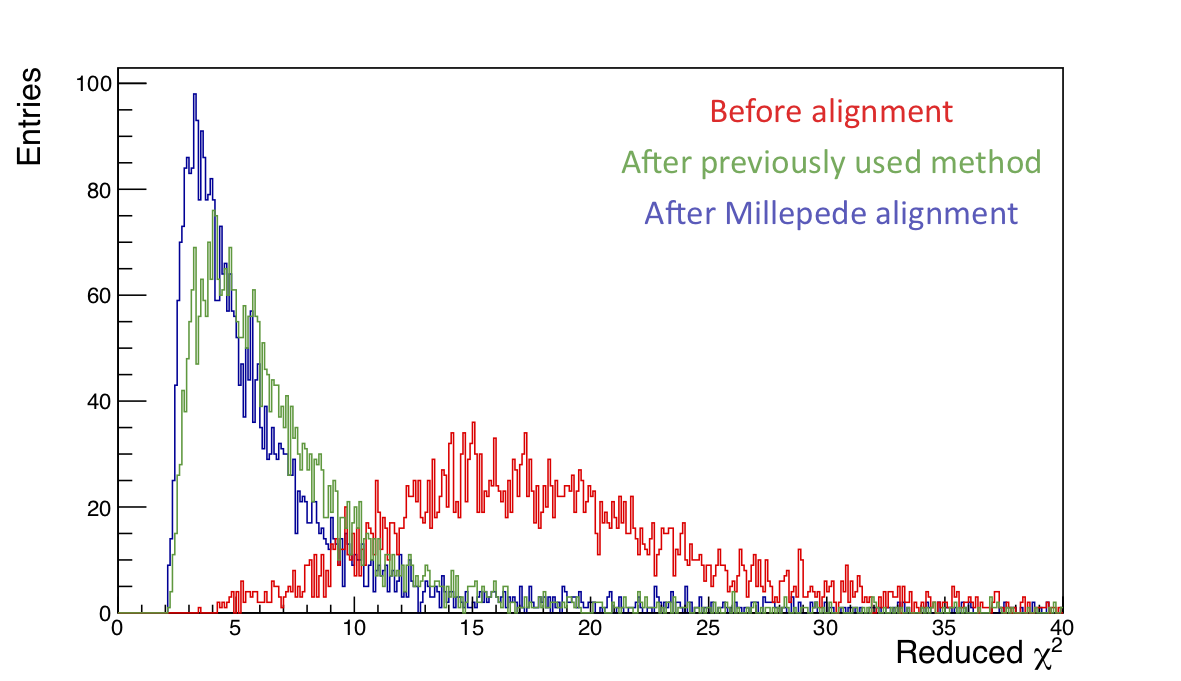
\includegraphics[width=0.85\textwidth]{thesis_figures/chi2_comp_conclusion_2.png}
% \caption{$\chi^2_{red}$ distribution for selected tracks showing the impact of Millepede alignment.}
% \label{fig:red_chi2_4}
% \end{figure}

Besides detecting ultra-high-energy (UHE) cosmic rays, the Pierre Auger Observatory with its large Surface Detector (SD) array offers a remarkable exposure to neutrinos above $10^{17}$eV. Any potential observation of such UHE$\nu_s$ will further our knowledge about the known universe. Since neutrinos are not deflected as they travel towards us at Earth, they offer a direct line of sight to the sources where they were produced. They are also some of the earliest particles produced in a transient source which makes their detection an important beacon for other astronomical instruments to perform a multi-messenger observation. The Pierre Auger Observatory is constantly monitoring the sky for the presence of such UHE$\nu_s$. The idea behind the detection remains the same as previous analysis at Auger where the neutrinos are assumed to induce Extensive Air Showers (EASs) close to the ground with a large electro-magnetic component at ground ("young" showers). This strategy is only employed for horizontal showers ($\theta > 60^{\circ}$). Two new SD triggers, time-over-threshold-deconvolved (ToTd) and multiplicity of positive steps (MoPS) were installed in 2014 to further increase the detection efficiency for low energy neutrino induced EASs. This thesis presents the first analysis of this improved efficiency for low energy neutrino showers in the zenith range $\theta \in [60^{\circ},75^\circ]$ also known as Down-going low or DG$_{Low}$ range. In this thesis the effect of the new triggers was evaluated for two types of searches, the searches for the diffused flux of UHE$\nu_s$ and search for point-like sources of UHE$\nu_s$. For both searches an overall improvement of efficiency is observed when information from the new triggers is incorporated in the analysis. A short summary of the three main contributions of this thesis along with an outlook detailing potential improvements are detailed in the next sections. 
\section*{Incorporating new triggers in the DG$\mathrm{_{low}}$ UHE$\nu_s$ searches}
During this thesis each facet of the DG$_{low}$ analysis was analysed. An effort was made to maximize the potential of the analysis. A blind search strategy similar to~\cite{gap_note_2013,Aab_2019_diffuse} was followed to avoid any bias in the analysis. The first step in this process was to include the information from the new triggers in the neutrino searches. About $\sim$7 years of recorded data was available for this task. The effect of the new triggers was first evaluated on neutrino simulations by including them in the analysis chain as described in section~\ref{subsubsec:nu_sel_fisher_training}. By the inclusion of new triggers an overall increase in reconstructed events was observed as shown in fig~\ref{fig:Events_vs_angle_summary}. This increase was most significant for lower energy neutrinos and decreased with increase in primary energy. This was an expected consequence due to the design of the new triggers. The overall increase also allowed for further modifications to the analysis which included lowering some stringent cuts as described in section~\ref{subsec:nu_sel_nudeteff}. For the final step of the analysis a Fisher discriminate polynomial was built and trained using the simulations (signal training sample) and a small fraction of recorded data, $\sim$20\% from the Observatory (background training sample). The polynomial is built with Area over Peaks (AoPs) of the stations and a differentiation between the background and signal is performed based on a cut on the Fisher value as given in eq.~\ref{eq:fisher_poly_cut}.
After the fixing the selection, a test sample was unblinded to catch any remaining flaws in the analysis. This proved worthwhile as a small error in the reconstruction was discovered during this process. The error was promptly corrected, and the whole selection procedure was re-evaluated, and the Fisher was retrained. Since the correction involved a change to the reconstruction procedure the blind search was redone from the start. After this correction the unblinding was again performed in two stages. The new test sample and the full blinded sample, 20\% + 60\% of recorded data between the period of 1 Jan 2014 to 31 December 2012 was analysed to search for neutrinos. \textbf{No neutrino candidates} were found in the search performed using the analysis described in this thesis. 

\subsection*{Outlook}
Even though a concerted effort was made to maximize the potential of the analysis presented in this thesis certain improvements could not be implemented and are thus summarized here for future studies. The segmentation algorithm used for reconstruction of events for neutrino searches was found to be not properly tuned for the new triggers, ToTd and MoPS. Thus, for this analysis the new triggers were completely removed from the segmentation algorithm. The primary purpose of the segmentation algorithm is to evaluate the correct start times for the WCD signals to decrease the effect of accidental muons which in turn affects the zenith angle estimation. A better tuned segmentation algorithm could thus further improve the neutrino search with new triggers. A more detailed summary of this topic along with examples of events where the segmentation algorithm fails and where it could help are presented in Appendix~\ref{sec:app_3}. This tuning could not be explored in this thesis but could be implemented in the future. Further, as seen in this analysis the angular reconstruction used for neutrinos is not particularly calibrated for EASs which originate deep in the atmosphere. This could also be rectified for the future to improve this analysis. Other techniques which involved computing the zenith angle via measuring the footprint of the shower cannot not be applied here due to the compact nature of EASs expected for the angular range explored. In this thesis a cut on the saturated and active PMTs was also explored but not implemented in the final analysis. A detailed study on such a cut could also be useful to increase the efficiency of the analysis. 

Further, work was done in this thesis to adapt the DG$_{high}$ analysis to the current $\mathrm{\overline{Off} \underline{line}}$ version which is detailed in Appendix~\ref{sec:app_4}. This work is still in progress and could be used in the future to evaluate and test potential improvements to the analysis. The impact of inclusion of new triggers for such an analysis is expected to be minimal due to their decreasing efficiency with increasing zenith angle. However, new triggers could still potentially improve the efficiency for neutrinos (E $\sim 10^{17}-10^{17.5}$eV) even in this angular range. 

\section*{Improvements to the diffuse flux limit for UHE$\nu_s$ with new triggers}
With no neutrino candidate detected a 90\% C.L. upper limit on the diffuse flux of UHE$\nu_s$ for the DG$\mathrm{_{low}}$ channel was evaluated. The limit was evaluated under the assumption of a diffuse flux given by $\mathrm{\phi \propto E_{\nu}^-2}$ with a 1:1:1 neutrino flavour ratio at earth. The integrated limit is given as:
\begin{equation}
    k_{90} < 1.9 x 10^{-17} \mathrm{GeV cm^{-2} s^{-1} sr^{-1}},
\end{equation}
in the energy range $E_{\nu} \in [1.3 \times 10^{18} - 2.5 \times 10^{19.5}]$eV. The integrated limit represents the value of the normalisation of the differential flux needed to predict $\sim$2.39 expected events. The number 2.39 was evaluated using a semi Bayesian extension of the Feldman \& Cousins treatment accounting for systematic uncertainties on exposure~\cite{Conrad:2002kn}. This limit is $\sim 40\%$ stricter than the one obtained without the new triggers for the same time period. Even though this improvement is significant 
\section*{Improvements to the point source searches for UHE$\nu_s$ with new triggers}
Further a point sensitivity comparison was also performed to evaluate the performance of the new triggers. The methodology was adopted from ~\cite{Aab_2019_point} and an energy and declination dependent exposure was evaluated for the DG$\mathrm{_{_low}}$ range. Using the no neutrino candidate detection ansatz, a 90\% C.L. upper limit on the neutrino flux from point-like sources as a function of source declination, $\delta$ was evaluated and presented in fig.~\ref{fig:Dec_limit_new old}. This limit was also shown to improve with the inclusion of new triggers. The improvement though small has an impact in the overall sensitivity since the different searches (DG$_low$, DG$_high$, ES) have different FOVs. It must also be stressed that Auger is one of the constantly running experiments sensitive to Energy ranges > $10^{18}$eV thus any improvement to its sensitivity is an important step for the potential future detection of UHE$\nu_s$.



%%% Local Variables:
%%% mode: latex
%%% TeX-master: "mythesis"
%%% End:

% Uncomment the following command to get references per chapter.
% Put it inside the file or change \include to \input if you do not want the references
% on a separate page
% \printbibliography[heading=subbibliography]

%------------------------------------------------------------------------------
% Use biblatex for the bibliography
% Add bibliography to Table of Contents
% Comment out this command if your references are printed for each chapter.
% \printbibliography[heading=bibintoc]

%------------------------------------------------------------------------------
% Include the following lines and comment out \printbibliography if
% you use BiBTeX for the bibliography.
% If you use biblatex package the files should be specified in the preamble.
\KOMAoptions{toc=bibliography}
{\raggedright
  \bibliographystyle{../refs/atlasBibStyleWithTitle.bst}
  %\bibliographystyle{unsrt}
  \bibliography{./thesis_refs,../refs/standard_refs-bibtex}
}

%------------------------------------------------------------------------------
\appendix
% \part*{Appendix}
% Add your appendices here - don't forget to also add them to \includeonly above
%------------------------------------------------------------------------------
\chapter{Alignment Figures}
\label{sec:app_1}
%------------------------------------------------------------------------------
This appendix includes the comparison of residuals obtained from alignment using the previously used method and Millepede. The reduced chi-square comparison plots for the two methods were shown earlier.
It also includes the residual versus position plots for the Micromega detectors.
\begin{figure}[h!]
\centering
 \begin{subfigure}[l]{.45\textwidth}
   \centering
   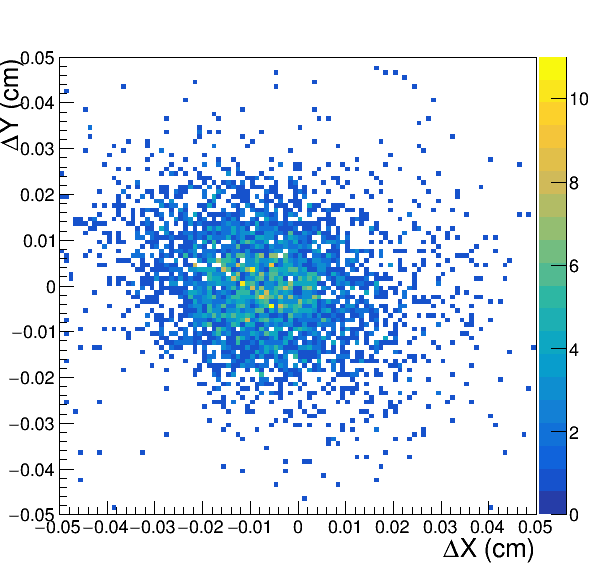
\includegraphics[width=\linewidth]{thesis_figures/alignment/Run_3211_after_prev/square/GEM1.png}

   \caption{GEM1 after previously used method}
   \label{fig:GEM1_after_prev}
 \end{subfigure}
 %\hfill
 \begin{subfigure}[r]{.45\textwidth}
   \centering
   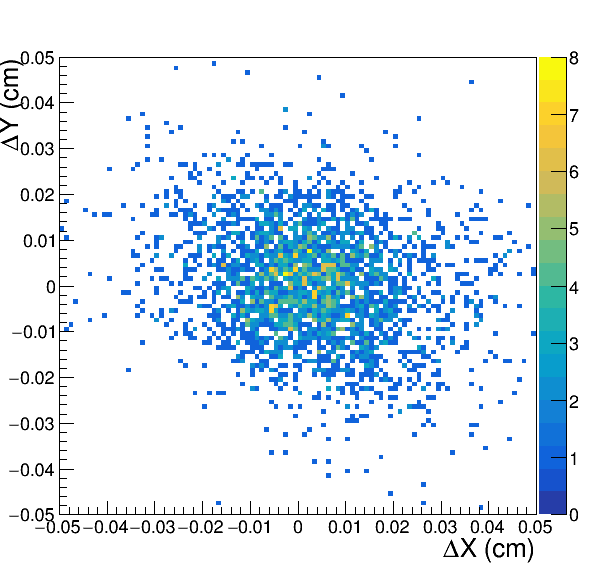
\includegraphics[width=\linewidth]{thesis_figures/alignment/Run_3211_after_millepede/square/GEM1.png}
   \caption{GEM1 after Millepede}
   %\label{fig:GEM1_before}
 \end{subfigure}
 \hfill
 \begin{subfigure}[l]{.45\textwidth}
   \centering
   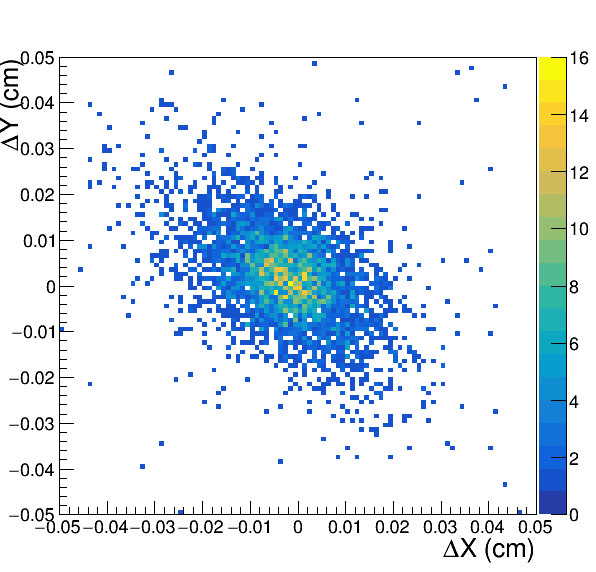
\includegraphics[width=\linewidth]{thesis_figures/alignment/Run_3211_after_prev/square/GEM2.png}
   \caption{GEM2 after previously used method}
   \label{fig:GEM2_after_prev}
 \end{subfigure}
 %\hfill
 \begin{subfigure}[r]{.45\textwidth}
   \centering
   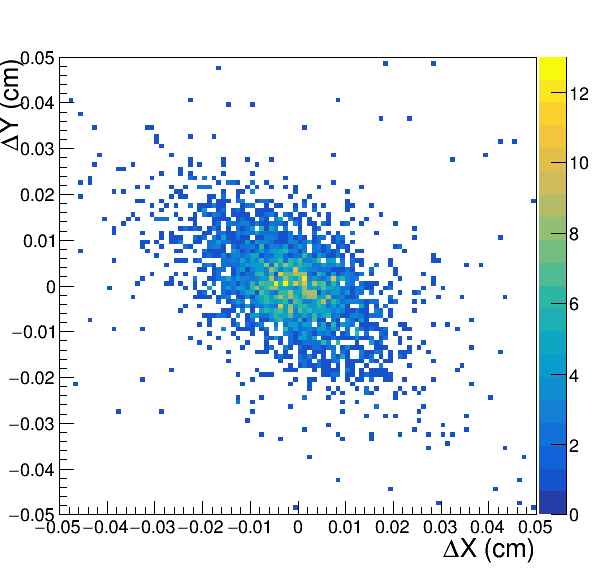
\includegraphics[width=\linewidth]{thesis_figures/alignment/Run_3211_after_millepede/square/GEM2.png}
   \caption{GEM2 after Millepede}
   %\label{fig:GEM2_before}
 \end{subfigure}
 \begin{subfigure}[l]{.45\textwidth}
   \centering
   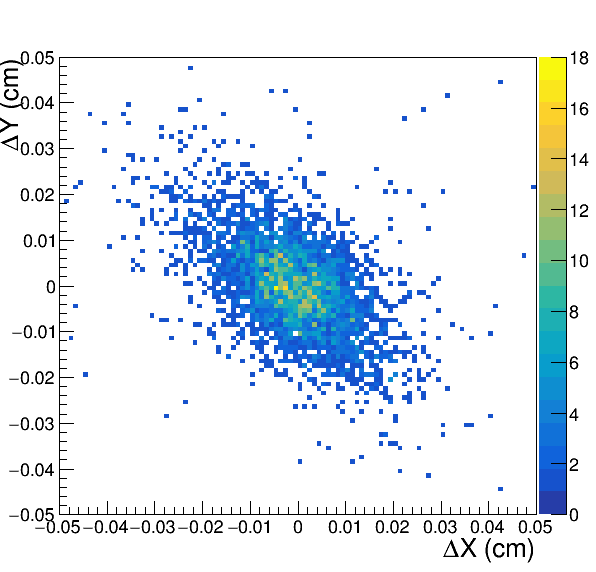
\includegraphics[width=\linewidth]{thesis_figures/alignment/Run_3211_after_prev/square/GEM4.png}

   \caption{GEM4 after previously used method}
   \label{fig:GEM4_after_prev}
 \end{subfigure}
 %\hfill
 \begin{subfigure}[r]{.45\textwidth}
   \centering
   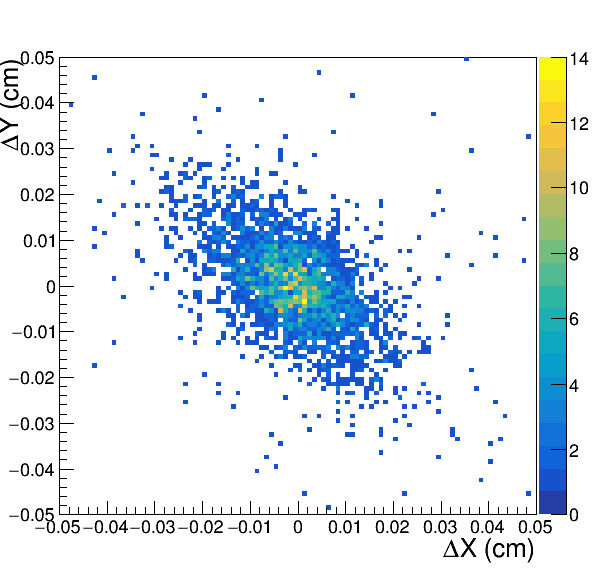
\includegraphics[width=\linewidth]{thesis_figures/alignment/Run_3211_after_millepede/square/GEM4.png}
   \caption{GEM4 after Millepede}
   %\label{fig:GEM4_before}
 \end{subfigure}
 \caption{Residual of GEM detectors.}
\end{figure}

%%%%MICROMEGAS start here

\begin{figure}[h!]
\centering
 \begin{subfigure}[l]{.45\textwidth}
   \centering
   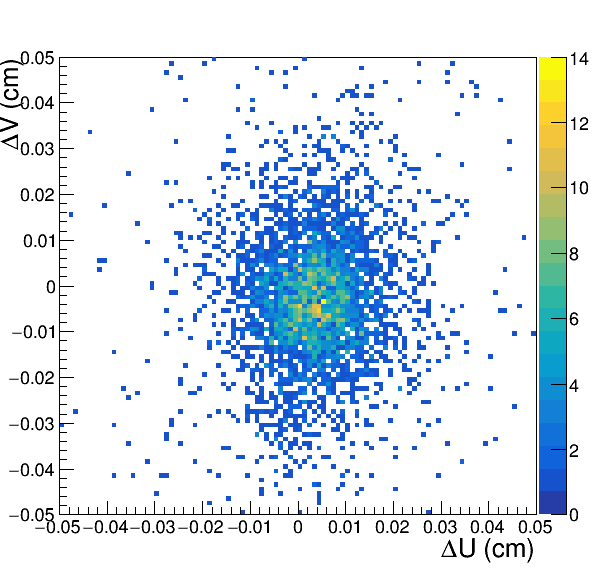
\includegraphics[width=\linewidth]{thesis_figures/alignment/Run_3211_after_prev/square/MX1.png}

   \caption{MM1 after previously used method}
   \label{fig:MX1_after_prev}
 \end{subfigure}
 %\hfill
 \begin{subfigure}[r]{.45\textwidth}
   \centering
   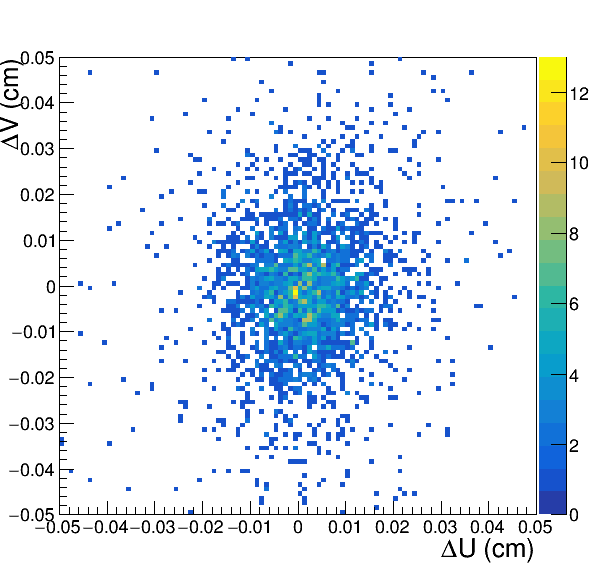
\includegraphics[width=\linewidth]{thesis_figures/alignment/Run_3211_after_millepede/square/MX1.png}
   \caption{MM1 after Millepede}
   %\label{fig:MX1_after}
 \end{subfigure}
 \hfill
 \begin{subfigure}[l]{.45\textwidth}
   \centering
   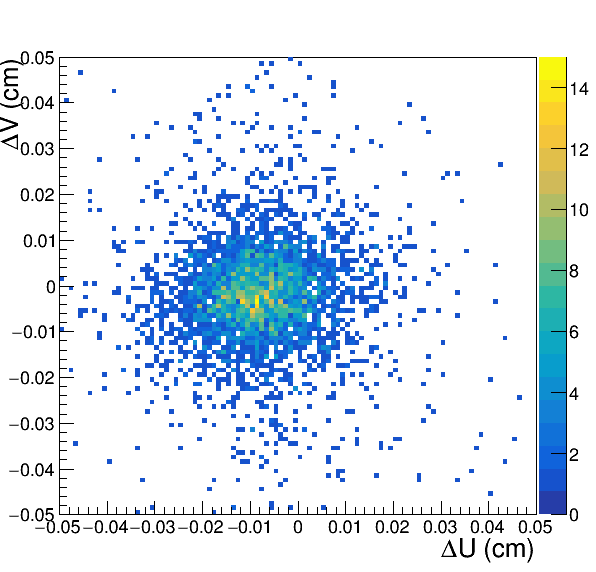
\includegraphics[width=\linewidth]{thesis_figures/alignment/Run_3211_after_prev/square/MX2.png}
   \caption{MM2 after previously used method}
   \label{fig:MX2_after_prev}
 \end{subfigure}
 %\hfill
 \begin{subfigure}[r]{.45\textwidth}
   \centering
   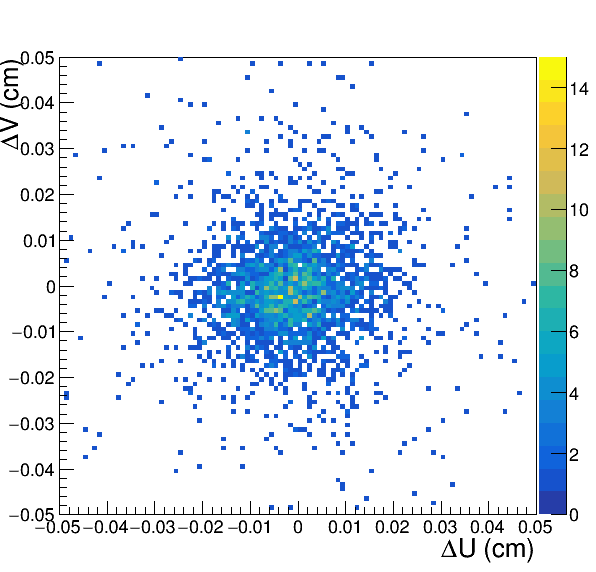
\includegraphics[width=\linewidth]{thesis_figures/alignment/Run_3211_after_millepede/square/MX2.png}
   \caption{MM2 after Millepede}
   %\label{fig:MX2_after}
 \end{subfigure}
 \begin{subfigure}[l]{.45\textwidth}
   \centering
   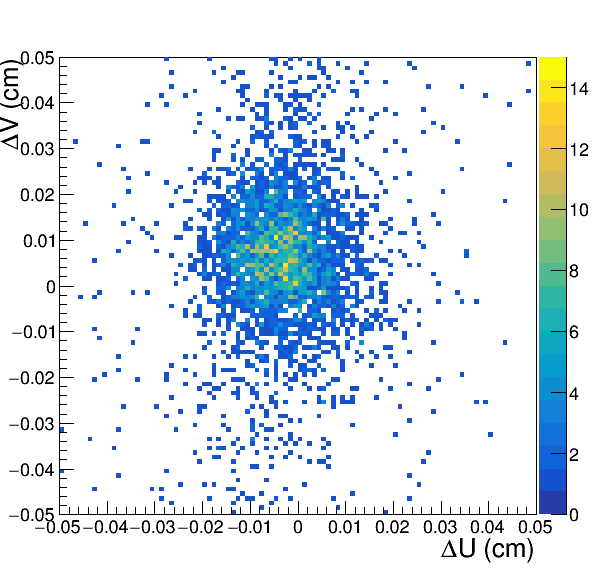
\includegraphics[width=\linewidth]{thesis_figures/alignment/Run_3211_after_prev/square/MX3.png}

   \caption{MM3 after previously used method}
   \label{fig:MX3_after_prev}
 \end{subfigure}
 %\hfill
 \begin{subfigure}[r]{.45\textwidth}
   \centering
   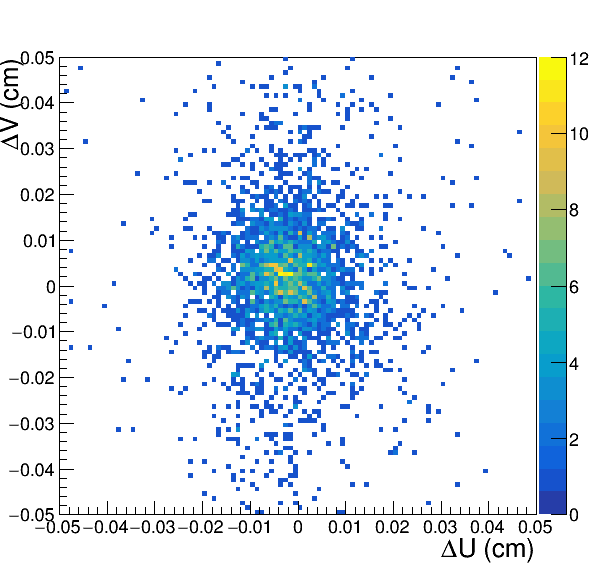
\includegraphics[width=\linewidth]{thesis_figures/alignment/Run_3211_after_millepede/square/MX3.png}
   \caption{MM3 after Millepede}
   %\label{fig:MX3_after}
 \end{subfigure}
 \caption{Residual of Micromega detectors.}
\end{figure}


\begin{figure}[h!]
\centering
 \begin{subfigure}[l]{.45\textwidth}
   \centering
   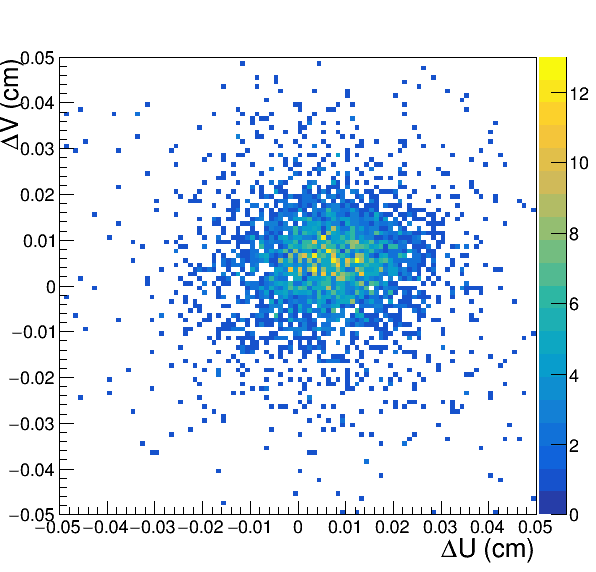
\includegraphics[width=\linewidth]{thesis_figures/alignment/Run_3211_after_prev/square/MX4.png}

   \caption{MM4 after previously used method}
   \label{fig:MX4_after_prev}
 \end{subfigure}
 %\hfill
 \begin{subfigure}[r]{.45\textwidth}
   \centering
   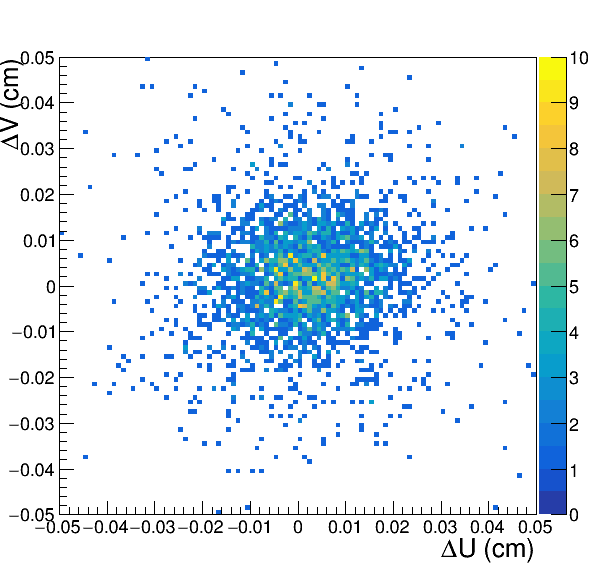
\includegraphics[width=\linewidth]{thesis_figures/alignment/Run_3211_after_millepede/square/MX4.png}
   \caption{MM4 after Millepede}
   %\label{fig:MX4_after}
 \end{subfigure}
 \hfill
 \begin{subfigure}[l]{.45\textwidth}
   \centering
   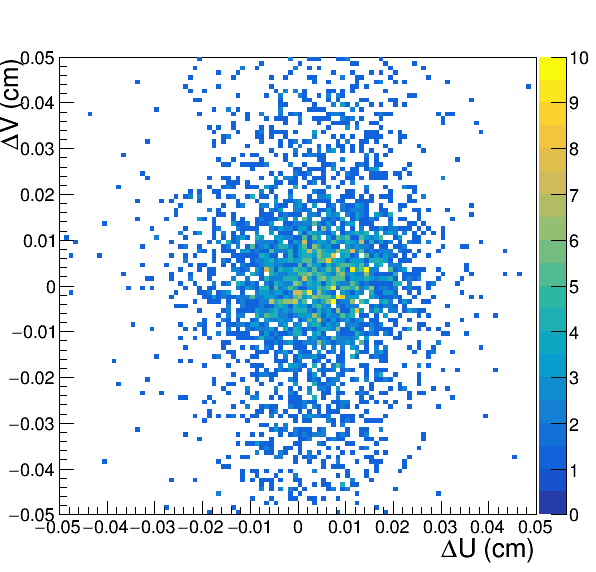
\includegraphics[width=\linewidth]{thesis_figures/alignment/Run_3211_after_prev/square/MX5.png}
   \caption{MM5 after previously used method}
   \label{fig:MX5_after_prev}
 \end{subfigure}
 %\hfill
 \begin{subfigure}[r]{.45\textwidth}
   \centering
   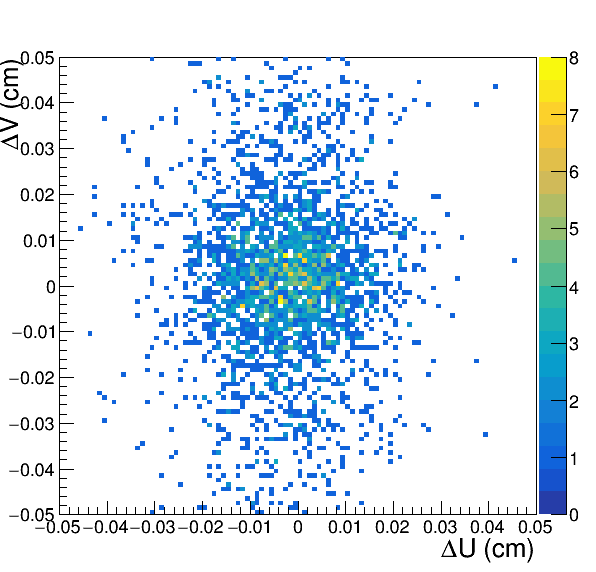
\includegraphics[width=\linewidth]{thesis_figures/alignment/Run_3211_after_millepede/square/MX5.png}
   \caption{MM5 after Millepede}
   %\label{fig:MX5_after}
 \end{subfigure}
 \begin{subfigure}[l]{.45\textwidth}
   \centering
   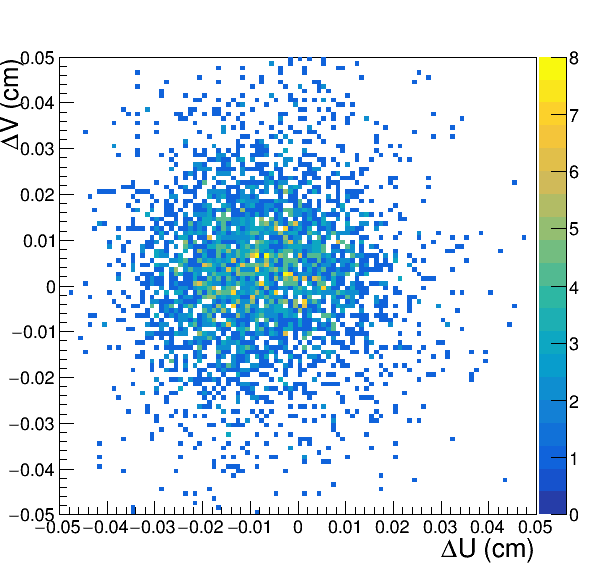
\includegraphics[width=\linewidth]{thesis_figures/alignment/Run_3211_after_prev/square/MX7.png}

   \caption{MM6 after previously used method}
   \label{fig:MX6_after_prev}
 \end{subfigure}
 %\hfill
 \begin{subfigure}[r]{.45\textwidth}
   \centering
   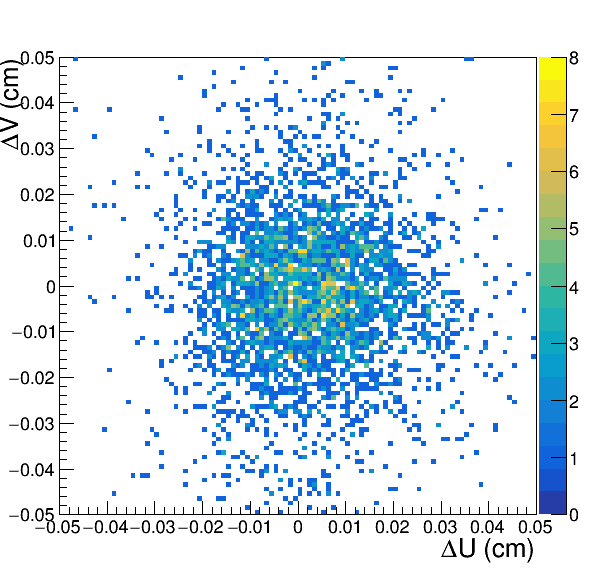
\includegraphics[width=\linewidth]{thesis_figures/alignment/Run_3211_after_millepede/square/MX7.png}
   \caption{MM6 after Millepede}
   %\label{fig:MX6_after}
 \end{subfigure}
 \caption{Residual of Micromega detectors.}
\end{figure}

%%micromegas%

\begin{figure}[h!]
\centering
 \begin{subfigure}[l]{.45\textwidth}
   \centering
   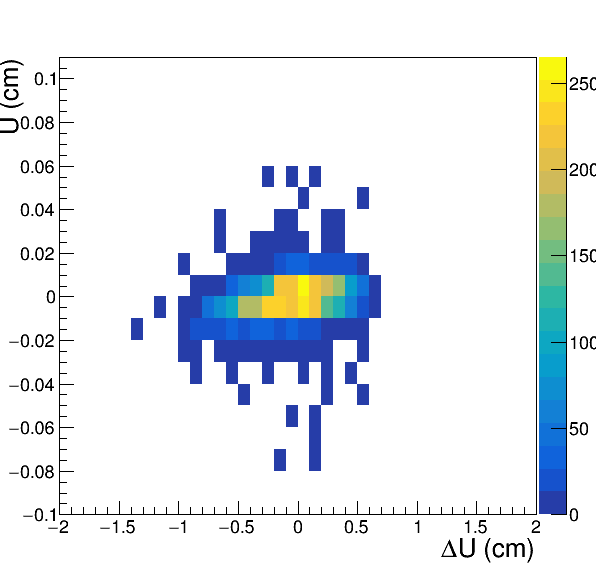
\includegraphics[width=\linewidth]{thesis_figures/alignment/Run_3211_T/rotMX1U_after_millepede_T.png}
   \caption{MM1 U plane}
   %\label{fig:MX1X_before}
 \end{subfigure}
 %\hfill
 \begin{subfigure}[r]{.45\textwidth}
   \centering
   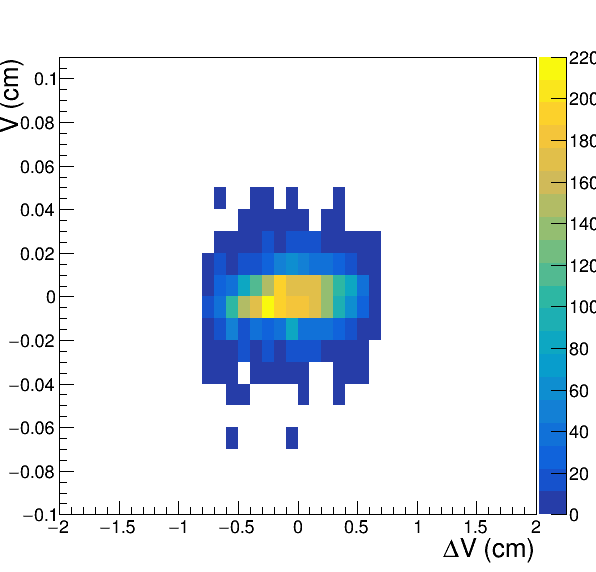
\includegraphics[width=\linewidth]{thesis_figures/alignment/Run_3211_T/rotMX1V_after_millepede_T.png}
   \caption{MM1 V plane}
   %\label{fig:MX1Y_before}
 \end{subfigure}
 \hfill
 \begin{subfigure}[l]{.45\textwidth}
   \centering
   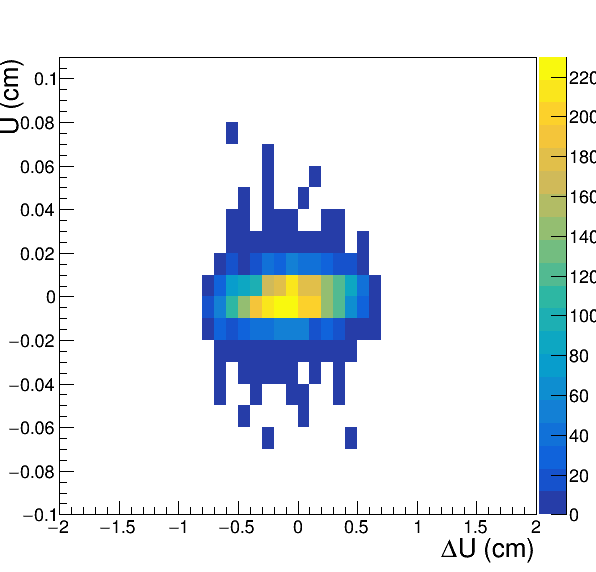
\includegraphics[width=\linewidth]{thesis_figures/alignment/Run_3211_T/rotMX2U_after_millepede_T.png}
   \caption{MM2 U plane}
   %\label{fig:GEM2X_before}
 \end{subfigure}
 \begin{subfigure}[r]{.45\textwidth}
   \centering
   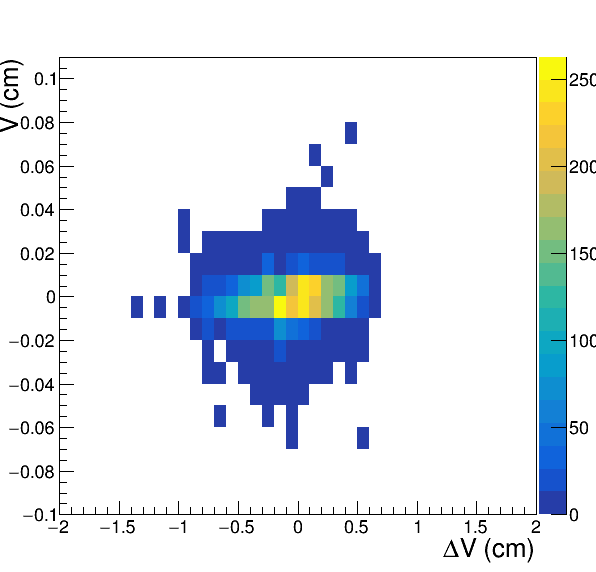
\includegraphics[width=\linewidth]{thesis_figures/alignment/Run_3211_T/rotMX2V_after_millepede_T.png}
   \caption{MM2 V plane}
   %\label{fig:GEM2Y_before}
 \end{subfigure}
 \hfill
 \begin{subfigure}[l]{.45\textwidth}
   \centering
   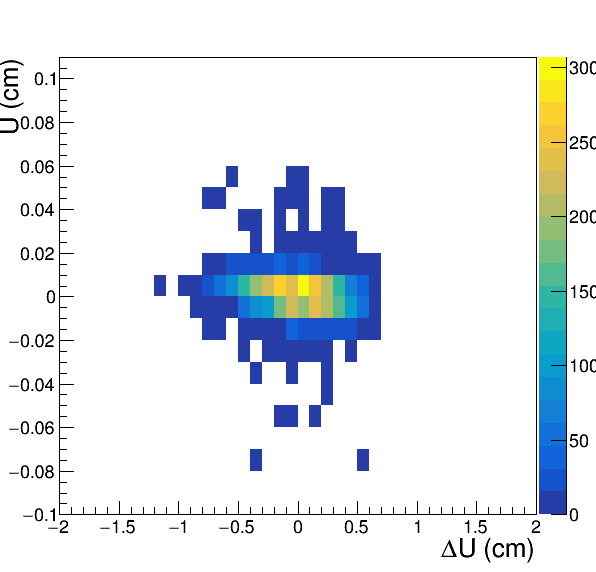
\includegraphics[width=\linewidth]{thesis_figures/alignment/Run_3211_T/rotMX3U_after_millepede_T.png}
   \caption{MM3 U plane}
   %\label{fig:MX1 X plane}
 \end{subfigure}
 %\hfill
 \begin{subfigure}[r]{.45\textwidth}
   \centering
   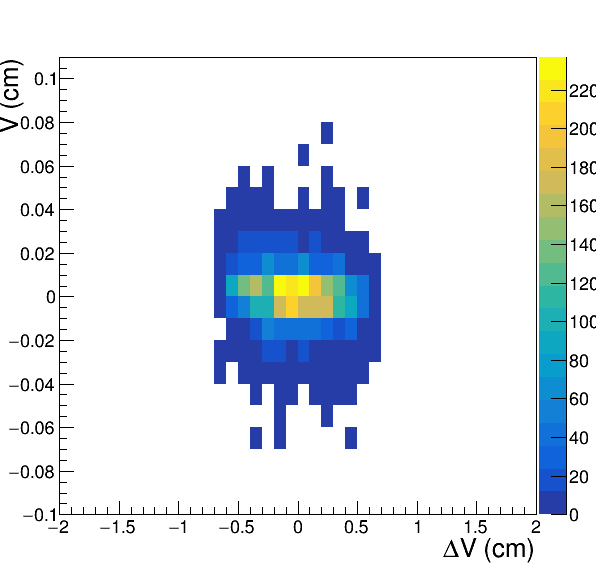
\includegraphics[width=\linewidth]{thesis_figures/alignment/Run_3211_T/rotMX3V_after_millepede_T.png}
   \caption{MM3 V plane}
   %\label{fig:GEM4Y_before}
 \end{subfigure}
 \caption{Residual vs position for Micromega detectors}
 \label{fig:res_vs_pos_MX}
\end{figure}

\begin{figure}[t!]
\begin{subfigure}[l]{.45\textwidth}
  \centering
  \includegraphics[width=\linewidth]{thesis_figures/alignment/Run_3211_T/rotMX4U_after_millepede_T.png}
  \caption{MM4 U plane}
  %\label{fig:GEM4X_before}
\end{subfigure}
%\hfill
\begin{subfigure}[r]{.45\textwidth}
  \centering
  \includegraphics[width=\linewidth]{thesis_figures/alignment/Run_3211_T/rotMX4V_after_millepede_T.png}
  \caption{MM4 V plane}
  %\label{fig:GEM4Y_before}
\end{subfigure}
\caption{ Residual vs position for MM4}
\end{figure}
%%% Local Variables:
%%% mode: latex
%%% TeX-master: "../mythesis"
%%% End:

%------------------------------------------------------------------------------
\chapter{Testing the impact of high and low energy hadronic interaction models for neutrino simulations}
\label{sec:app_2}
%------------------------------------------------------------------------------
This appendix contains the efforts done to check the dependence of the low and high hadronic interaction models used to simulate neutrino showers. The check was performed before the full library was simulated by the MC task. For the choice of the low energy hadronic interaction model UrQMD and FLUKA were compared and for the high energy model QGSJET-II-04,EPOS-LHC and SIBYLL 2.3d  were compared. The comparison was done by simulating 20 neutrino showers for each model for five different injected slant depths. The comparison was only done for $\nu_e$ CC showers with a primary energy of $10^{19}$eV for a zenith angle of $72^\circ$ was considered for the comparison. These three choices were made since such neutrinos are expected to give a good idea of the performance of the models and their effect to the overall analysis. The showers were simulated with CORSIKA 7.7.2 and the output was fed to the Offline analysis framework for the detector response simulation and reconstruction in the same way as described in chapter.~\ref{chap:DGL}. 

The comparison was done by calculating the ratio of the surviving events for both the models at each simulated slant depth. This comparison is shown in fig.~\ref{fig:Efficiency_vs_slant_comp_FLUKAnURQMD}. As seen in the figure the ration $\sim 1$ within the error bars which are high due to lack of statistics. After this comparison FLUKA was chosen as the main low energy hadronic model used in the simulations mainly because of ease of use. 

\begin{figure}[ht!]
  \centering
  \includegraphics[width=\textwidth]{thesis_figures/App2/Efficiency_vs_slant_comp_FLUKAnURQMD.pdf}
  \caption{Ratio FLUKA vs URqmd}
  \label{fig:Efficiency_vs_slant_comp_FLUKAnURQMD}
\end{figure}


For the choice of high energy interaction model The T3 and $\nu$ identification efficiency was calculated. The T3 efficiency was calculated as a ratio of the number of reconstructed events to the number of simulated events. The $\nu$ identification efficiency was not calculated according to the method presented in this thesis but rather with a less stringent cut where the AoP of the three earliest stations were required to be above 1.5. The efficiency was calculated relative to the total simulated events and was plotted against the different injected slant depths which were simulated. This was also done to attempt to calculate the systematic uncertainties which can arise due to the choice of the hadronic interaction model. The systematic uncertainties were calculated as the difference between the integral of efficiencies of the different models. Taking SIBYLL 2.3d as the reference model A, to test any other model the uncertainty is given by $\frac{\int A - \int B}{\int B}$. The results of the comparison are shown in fig.~\ref{fig:Eff_vs_slant_comp_all_HModels}. The calculated systematic uncertainties are below 5\% for the T3 efficiency and below 10\% for the $\nu$ identification efficiency. The relative uncertainty for the T3 efficiency for SIBYLL 2.3d in comparison to the EPOS-LHC was found to be $\sim +3\%$ and for QGSJETTII04 was found to be $\sim + 7\%$ and the uncertainty on $\nu$ identification was found to be $\sim +10\%$ for both the models. However, due to the limited statistics no relevant conclusions can be drawn from this comparison. Thus, in the end the systematic uncertainties that were used in this analysis related to the choice of the hadronic interaction model were taken from other sources.  

\begin{figure}[h!]
  \centering
  \includegraphics[width=\textwidth]{thesis_figures/App2/Efficiency_vs_slant_comp_FLUKAnURQMD.pdf}
  \caption{All model eff comp}
  \label{fig:Eff_vs_slant_comp_all_HModels}
\end{figure}


% \printbibliography[heading=subbibliography]

%------------------------------------------------------------------------------
% Declare lists of figures and tables and acknowledgements as backmatter
% Chapter/section numbers are turned off
\backmatter

\listoffigures
%\listoftables

%------------------------------------------------------------------------------
% Print the glossary and list of acronyms
% \printglossaries

%------------------------------------------------------------------------------
% You could instead add your acknowledgements here - don't forget to
% also add them to \includeonly above
% %------------------------------------------------------------------------------
\chapter*{Acknowledgements}
\label{sec:ack}
%------------------------------------------------------------------------------
Even though this thesis has my name on the front a number of people were involved in shaping its final form both in person and in spirit.

First and foremost I would like to thank my late grandfather Shanti Sarup Sehgal and grandmother Kusum Sehgal. Their constant motivation and belief in my abilities has and will always inspire me to achieve more.

I am very grateful to Professor Bernhard Ketzer for giving me an opportunity to write my thesis in his group. In spite of my many shortcomings and failures he has always been patient and supportive during the entire time and has been a role model I look up to. I would also like to thank Professor Jochen Dingfelder. I have always admired your lectures and am thankful that you agreed to be my second supervisor.

A special thanks to PhD students Michael Hösgen and Martin Hoffmann for helping with the editing of this thesis. Thank you to Michael for always answering my various questions and solving my problems without which this thesis would have never been completed. A big thanks to the whole AG Ketzer group for both the academic and moral support.

I am grateful to my father Ravi Sehgal, my mother Rajni Sehgal and my brother Sambhav for all the sacrifices they have made. Without their constant support studying at Bonn would have just remained a pipe dream. Lastly, I am thankful to the wonderful set of friends I am lucky to have. Thank you Svenja ,Georgios and Amitayus for the countless Mensa lunches which helped me remain sane throughout the thesis.

%%% Local Variables:
%%% mode: latex
%%% TeX-master: "../mythesis"
%%% End:


%------------------------------------------------------------------------------
% CV needed when you submit your PhD thesis
% \definecolor{lightgray}{gray}{0.8}
\newcolumntype{L}{>{\raggedleft}p{0.15\textwidth}}
\newcolumntype{R}{p{0.8\textwidth}}
\newcommand\VRule{\color{lightgray}\vrule width 0.5pt}

\thispagestyle{empty}
\section*{Curriculum Vitae}

\subsection*{Personal Details}

\begin{tabular}{L!{\VRule}R}
Name & Johann Schmidt \\
Date of Birth &  \\
Email & abc@physik.uni-def.de \\
Family status & Single
\end{tabular}

\subsection*{Education}

\begin{tabular}{L!{\VRule}R}
1997--2003 & Abitur, ABC Secondary School, Hamburg, Germany\\
2004--2007 & BSc in Physics, Rheinische Friedrich-Wilhelms-Universität, Bonn, Germany.\\
2006 & CERN Summer Student, Geneva, Switzerland. \\
2007--2009 &  MSc in Physics Rheinische Friedrich-Wilhelms-Universität, Bonn, Germany. \\
2009--2012 &  PhD in Physics, Rheinische Friedrich-Wilhelms-Universität, Bonn, Germany. \\
2012 & Advanced Data Analysis School, Frankfurt, Germany.
\end{tabular}

\subsection*{Professional Experience}

\begin{tabular}{L!{\VRule}R}
2004 & Summer Student at CERN, Geneva, Switzerland. \\
2007--2012 & Doctoral work at the University of Bonn, Germany. \\
2008--2009 & Fieldwork at CERN, Geneva, Switzerland.\\
2011 & Talk at the Advanced Physics Conference, Timbucto
\end{tabular}

\subsection*{Languages}
\begin{tabular}{L!{\VRule}R}
German & Mother tongue \\
English & Fluent \\
Russian & Basic
\end{tabular}


\end{document}

%%% Local Variables:
%%% mode: latex
%%% TeX-master: t
%%% End:
